\chapter{Data Analysis I: Calibration and Corrections}

Need to explain pedestal subtraction 

\section{Software}
\label{sec:software}

The S$\pi$RITROOT software is modular tasked based code based on the FAIRROOT package written in C++ \cite{fairroot}. The main tasks in the S$\pi$RITROOT software reconstruction are:
\begin{itemize}
  \item Decoder task
  \item Pulse Shape Algorithm (PSA Task)
  \item Helix Track Finding Algorithm
  \item Clustering Algorithm
  \item Track Fitting (GENFIT package)
  \item Vertex Fitting (RAVE package)
\end{itemize}

The decoder task converts the binary data file into a container class which maps the electronics channels into the corresponding pads and (x,z) coordinates. 

There may be several pulses in a pad coming from two tracks passing under the same pad separated  by arrival time. Using an expected pulse shape the PSA task fits the signal pulses within a pad, giving the arrival time of the drifted electrons from each particular track. The height of the fitted pulse is proportional to the total charge of that event, Q and the y-coordinate is calculated as $y = v\cdot t_0$ where $v$ is the drift velocity and $t_0$ the arrival time. Combining the information from these first two tasks, (x,y,z,Q), we construct what is called a "hit". 

 The Helix Track Finding Algorithm finds the collection of hits belonging to one track out of all the hits in an event. The hits within a track are then reduced into clusters. A cluster's position is the average position of the hits within a cluster, with the total charge of the cluster being the sum of the hits charges. 
 
 A tracks average position is estimated by the cluster's average position. The clusters are then fitted in the GENFIT track fitting package \cite{genfit}, giving the final momentum of the track. A final vertex of the event is fitted from all tracks using the package RAVE \cite{rave}. 

\paragraph{Definition of clustering}

A brief description of the method of clustering is illustrated in Figure \ref{fig:topview}. It is impractical to cluster in both the x and z-axis and we only cluster the hits along one axis. The three clusters at the bottom of Figure \ref{fig:topview} are clustered along the x-axis and the upper three are along the z-axis, as shown by the bolded pads for one of the clusters in each direction.

 The clustering direction depends on the angle  of the track with respects to the x-axis, defined as $\theta$. For example, a track going along the z-axis the crossing angle is defined as $90^{\circ}$, and a track going along the x-axis defined as $0^{\circ}$. In the case that the crossing angle is $45^{\circ} < \theta \leq 90^{\circ} $ the clustering direction is along the x-axis. For $0^{\circ} < \theta \leq 45^{\circ}$ it is along the z-axis. 

 The position along the clustering direction is calculated by weighting the individual hit's positions by their charges $q_i$ and getting the mean value. The other direction is set to the center of the pad. For example if we are clustering along the x-axis for a cluster, the z-position is set to the center of the pad in the z-direction and vice versa. 

Clustering in this way gives us better position resolution for calculating the position of each cluster. You could imagine if we calculated the clusters only along the x-axis for tracks with $\theta \approx 0^{\circ}$ the x-position is not well defined. By clustering in the direction most perpendicular to the track, we get a better position resolution.

\begin{figure}[H]
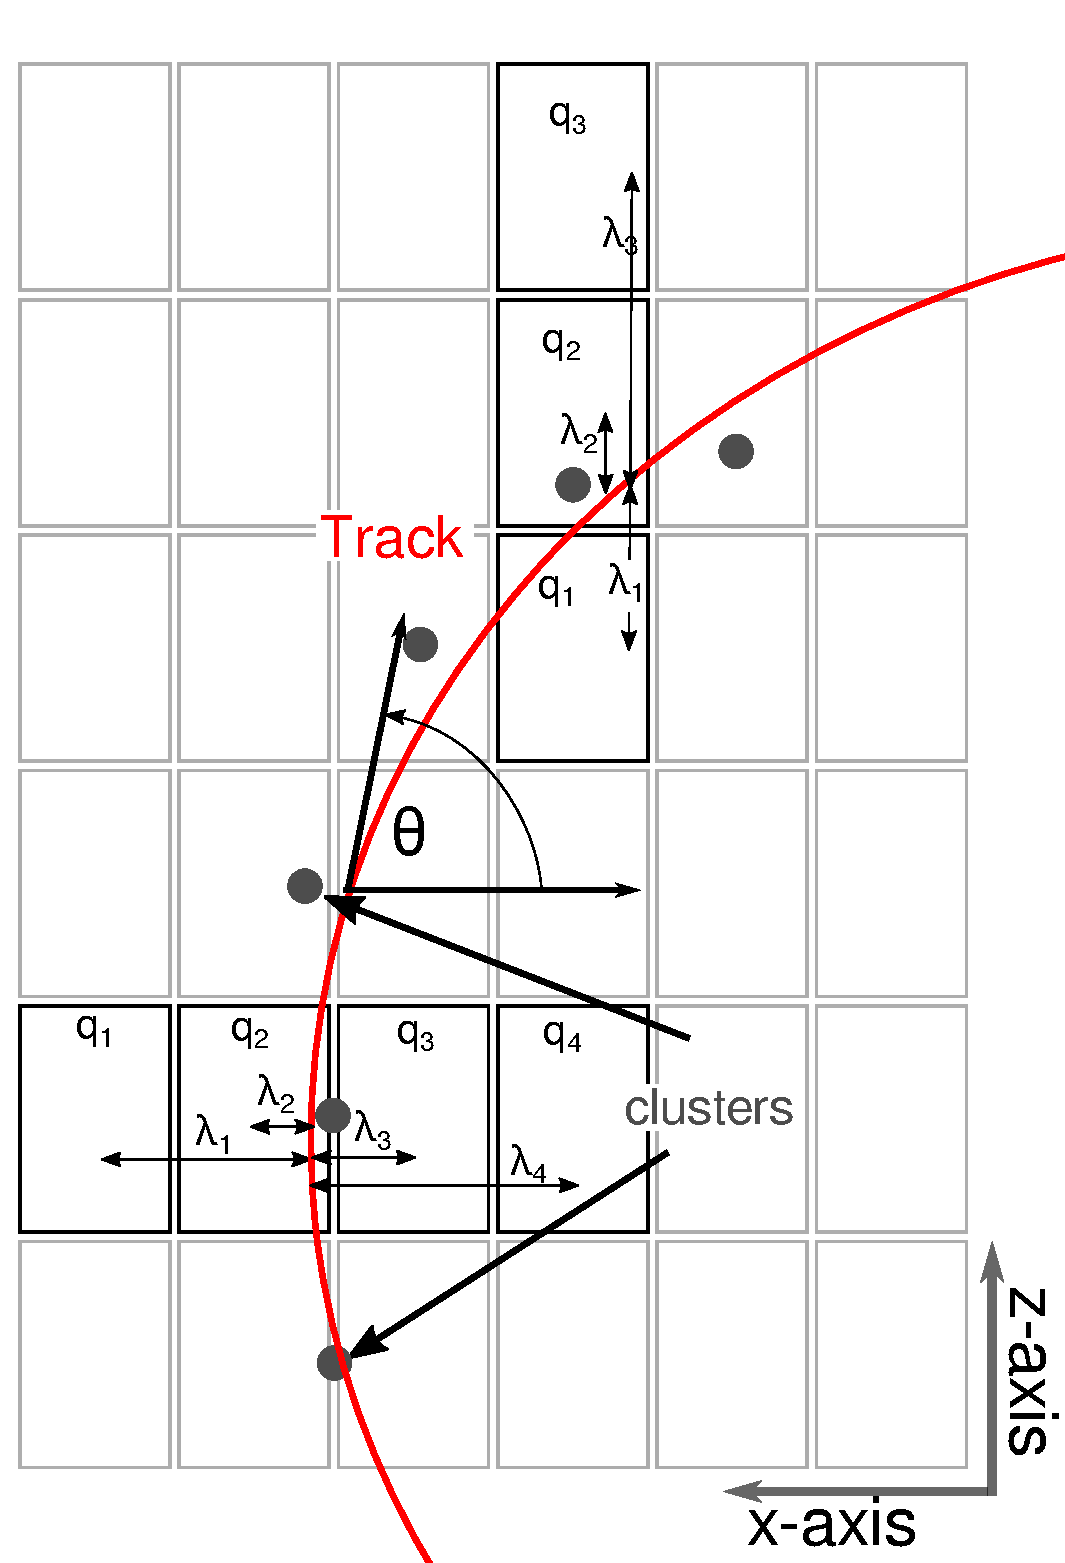
\includegraphics[scale=.5]{top_view_helix_ext.pdf}
\caption{Cartoon graphic of a top down view of a fit to a track passing through several pads. The bolded pads and the charges $q_i$ represent the hits belonging to that pad and the clusters of the track representing the average position of the track. The three clusters at the bottom are clustered in the x-direction and for the upper three clustered in the z-direction. The estimate of the position of the avalanche is given by the track fit and the position from the center to each pad to the $\bar{x}$ position is given as $\lambda_i$.}
\label{fig:topview}
\end{figure}


\subsection{Pulse Shape Algorithm}
\label{sec:psa}

\section{Calibrations and Corrections}


\subsection{Gating grid noise subtraction}
Opening the gating grid essentially short adjacent wires together allowing them to reach equilibrium as fast as possible. In practice the impedance of both sides was not entirely matched properly and this caused an oscillating current to bounce back and forth in an under-dampened manner. This caused residual induced signals early in the time bucket spectrum which created and extra source of noise in the data. The ground grid shielded some of the noise, but the path to ground was on two ends and was not sufficiency for this frequency. Figure~\ref{fig:ggNoiseSub} shows in the upper panel the gating grid noise ADC time bucket spectrum for 2000 events in a given pad. The signal is stable within a pad and the mean value --shown as the red line-- can be calculated after averaging over several thousands events. The raw gating grid noise lasts for 100 tbs extending into the real data with a decreasing amplitude. 

\begin{figure}[!htb]
\centering
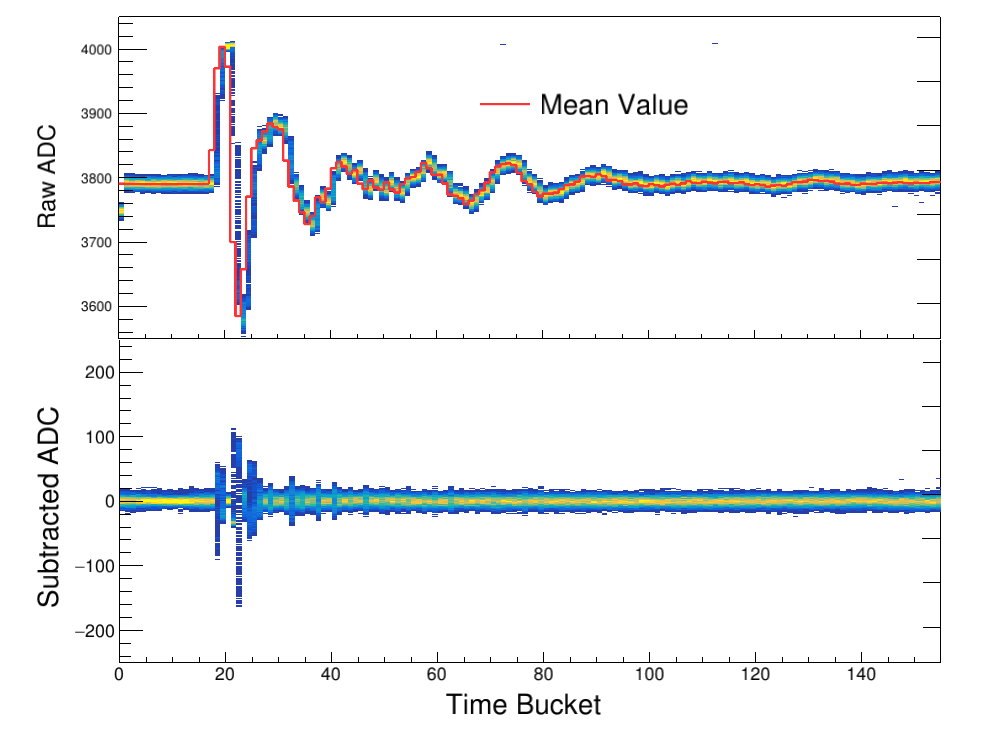
\includegraphics[width=\textwidth]{ggNoise.png}
\caption{Gating grid noise profile and subtraction for a particular pad.}
\label{fig:ggNoiseSub}
\end{figure}


The gating grid itself was not always stable an only the ${}^{132}$Sn and ${}^{124}$Sn beams were relatively stable. Several times during the ${}^{108}$Sn and ${}^{112}$Sn beams the gating grid broke. After several data runs were taken, we took what is called gating grid noise runs to get the profile of the gating grid noise throughout the experiment. To achieve this the anode wires would be turned off and the trigger was allowed to otherwise operate normally, firing the gating grid to open as usual. Since the anode wires were all turned off no signals would be seen except those coming from the gating grid noise. Several thousand triggers of the gating grid were taken to get a good noise profile. 

Once the mean value response in each pad is calculated, we can use the gating grid noise profile runs to correct the real data and remove the noise of the gating grid. To show the best case scenario of this technique, the bottom panel of Fig.~\ref{fig:ggNoiseSub} shows the gating grid noise self correcting itself. We can see the pedestal is already subtracted naturally when using this technique, and the subtracted ADC spectra is centered around 0. Residual gating grid noise that was not canceled by the subtraction remains but is significantly reduced to a much smaller time bucket region. This happens in regions where the gating grid noise is changing rapidly, where the ADC value is dependent upon small jitters in the timing of the signal. All time buckets below 30 tb were cut away from the spectrum to get rid of the small region where the gating grid is still opening and to remove the residual noise. 


%The average noise profile was constructed by averaging all the events in the gating grid runs, pad-by-pad; each pad had a slightly different noise profile since the impedance to each pad was slightly different. It is worth noting that the small electronics noise would be effectively canceled out by averaging over thousands of events. During the first stages of the software, the gating grid noise profile closest to that run would be subtracted from the raw data canceling the gating grid noise in that run. 

\subsection{Cocktail calibration}

\begin{table*}\centering
\ra{1.3}
\begin{tabular}{@{}rrrrrrr@{}}\toprule
& \multicolumn{3}{c}{$100 MeV Target$}\\
\cmidrule{2-4}
Particle &\phantom{abc} & Measured & Corrected & \% Difference & \% Difference\\
\midrule
p   & 882.8 & 929.5 & 877.3   &  3.7  & -1.0  \\
d   & 817.1 & 831.15 & 797.94 &  1.7  & -2.3\\
\bottomrule
\end{tabular}
\caption{Summary of expected cocktail. }
\label{tb:cocktail100tar}
\end{table*}

\begin{table*}\centering
\ra{1.3}
\begin{tabular}{@{}rrrrrrr@{}}\toprule
& \multicolumn{3}{c}{$100 MeV$}\\
\cmidrule{2-4}
Particle & Expected & Measured & Corrected & \% Difference & \% Difference\\
\midrule
p   & 882.8 & 903.5 & 889   &  2.0   & -1.6  \\
d   & 817.1 & 898.5 & 874.5 &  2.1   & -2.7\\
\bottomrule
\end{tabular}
\caption{Summary of expected cocktail. }
\label{tb:cocktail100}
\end{table*}

\begin{table*}\centering
\ra{1.3}
\begin{tabular}{@{}rrrrrrr@{}}\toprule
& \multicolumn{3}{c}{$300 MeV$}\\
\cmidrule{2-4}
Particle & Expected & Measured & Corrected & \% Difference Raw & \% Difference Corrected\\
\midrule
d   & 1621 & 1704 & 1612   &  5.1 & -0.6  \\
t   & 1612 & 1691 & 1596   &  4.9  & -1.0\\
${}^{4}$He   & 1613 & 1698 &  5.3 & 1595  & -1.1\\

\bottomrule
\end{tabular}
\caption{Summary of expected cocktail. }
\label{tb:cocktail300}
\end{table*}

A cocktail of several light charged particles were produced (p,d,t,${}^{3}$He,${}^{4}$He), and measured in the TPC to provide a momentum calibration of the TPC. The magnetic and slit settings of the dipoles in the BIGRIPS spectrometer was set so that the measured momentum resolution of the beam was $\delta p/p$ < 1\%. Two magnetic rigidity settings were studied, with an empty target. A thick Aluminum target was used to provide a slightly lower energy point for part of the lower rigidity setting, effectively creating three calibration points over several particle species. The production of certain particles (t,${}^{3}$He), produced too few counts to make a good measurement, and in the high momentum rigidity setting protons could not propagate down the line and there were no counts. 

Since the expected momentum resolution resulting from the spectrometer was less than 1\%, the observed momentum resolution measured by the TPC is a good representation of the combined momentum resolution of the software and TPC (intrinsic detection) system. The momentum resolution depends on several factors such as the particle's angle, momentum, charge, track multiplicity, etc. This calibration beam represents and ideal situation where the track was parallel to the pad plane and only one particle was measured at one time. The energy loss resolution can also be directly measured since each energy setting represents a monochromatic source of each particle species, which has a well defined energy loss distribution. An average momentum resolution of $dp/p = 2\%$ and the energy loss resolution of $d\langle dE/dx \rangle/\langle dE/dx \rangle = 5\%$ was measured for particles ranging from $H$ to ${}^{4}$He, over the range of momenta measured in the calibration beam as summarized in Table~\ref{tb:momresolution}.

Since the magnetic dipole setting of the BIGRIPS spectrometer defined the energy of each particle type, we can calculate the expected momenta of each particle species measured. Small corrections were propagated using LISE++ software which can calculate the energy loss through several materials in the beam line. These corrections resulted in a small change in the momenta. The measured momenta of the calibration beam differed significantly from the expected values as seen in Tables~\cref{tb:cocktail100tar,tb:cocktail100,tb:cocktail300}. This effect is attributed to inhomogenatities in the magnetic field which introduces electron drift velocity in the direction of $\vec{E}\times\vec{B}$ direction as seen from Eq.\ref{eq:elecdrift}. The $\vec{E}\times\vec{B}$ drift velocity causes the electron trajectories to shift toward the +x-axis in the TPC coordinates causing particles of positive charge (going in the -x-axis) to have a higher measured momenta than in reality. The disagreement in measured and expected momenta is upwards of ~5\% difference in the higher momentum calibration settings. The details of the correcting for the $\vec{E}\times\vec{B}$ effect will be discussed in the later Section~\ref{sec:spacecharge} in a more general way which also includes correction for the space charge, which this cocktail beam does not have. The same correction technique was applied here in the special case of zero space charge, which is the special case of only having $\vec{E}\times\vec{B}$ components.

The values under the corrected column seen in Tables~\cref{tb:cocktail100tar,tb:cocktail100,tb:cocktail300}, represent the data corrected for the $\vec{E}\times\vec{B}$ effect. A significant improvement is seen in the high momentum setting going from around ~5\% disagreement to within ~1\% agreement in the corrected data. For the lower momentum settings (Tables~\cref{tb:cocktail100tar,tb:cocktail100}), protons see a slight improvement of about ~1\% where as the deuterons are over corrected in both settings. The level of agreement of the all corrected values is still within the estimated momentum resolution of the TPC. 

\begin{table*}\centering
\ra{1.3}
\begin{tabular}{@{}rr@{}}\toprule
Momentum Resolution \% & <dE/dx> Resolution \% \\
\midrule
1.6  & 4.6\\
\bottomrule
\end{tabular}
\caption{Summary of expected cocktail. }
\label{tb:momresolution}
\end{table*}

%Apendix of the beam line elements
%apendix of the settings of the bigrips elments
%Picture of cocktail before and after ExB effect
%Table of LISE++ expected cocktail energies ridigity setting of dipole magnets (reference big rips line)


\subsection{Electronics calibration}
The ADC channel number of the electronics was calibrated by measuring the response of each channel to an input pulse supplied by a pulse generator. The pulse was distributed to all the electronics channels by pulsing the ground plane for a range of input voltages. This distributed the pulse evenly across the entire pad plane. The input voltage is plotted as a function of the measured ADC channel in Fig.~\ref{fig:gaincalib} for every channel. The small variation in each channel can be seen as the wide band around each measurement point. A linear fit is performed to get the best fit line which provides a reference line which each channel is calibrated to. The right panel shows the resulting distribution of channels after calibration. This is a relative calibration technique with the intent to calibrate the varying gains in each channel relative to one another. 

\begin{figure}[H]
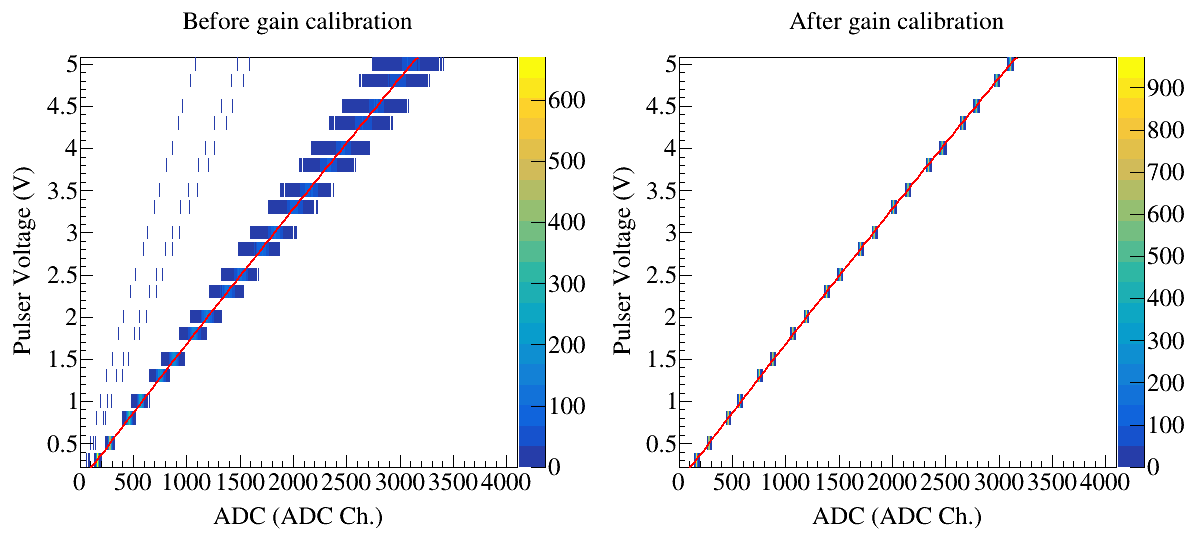
\includegraphics[width=\linewidth]{gaincalib.png}
\caption{Calibration of electronics}
\label{fig:gaincalib}
\end{figure}

\subsection{Anode gain calibration}

As mentioned earlier, the anode wires were separated into 14 independently biased sections. The high voltage of sections 12 and 14 were reduced during the experiment due to high currents being observed on the wires. The wire section voltages were lowered once and adjusted once again. Out of all the runs used in the analysis in this thesis \ref{tb:runList}, the anode sections 12 and 14 were lowered to \SI{1085}{\volt} for runs 2272-2371 and set to \SI{1214}{\volt} for all the other runs. By lowering the voltage on these anode wires, the gas gain is lowered as compared with all the other anode wire plane sections which operate at \SI{1460}{\volt}. To account for the drop in gain, in the software we increase the gain of the pads which lie above these anode wires to match the gain in the other channels. To do so, we compare the energy loss in the high gain sections to the low gain sections to get the relative calibration factor. 


\begin{figure}[H]
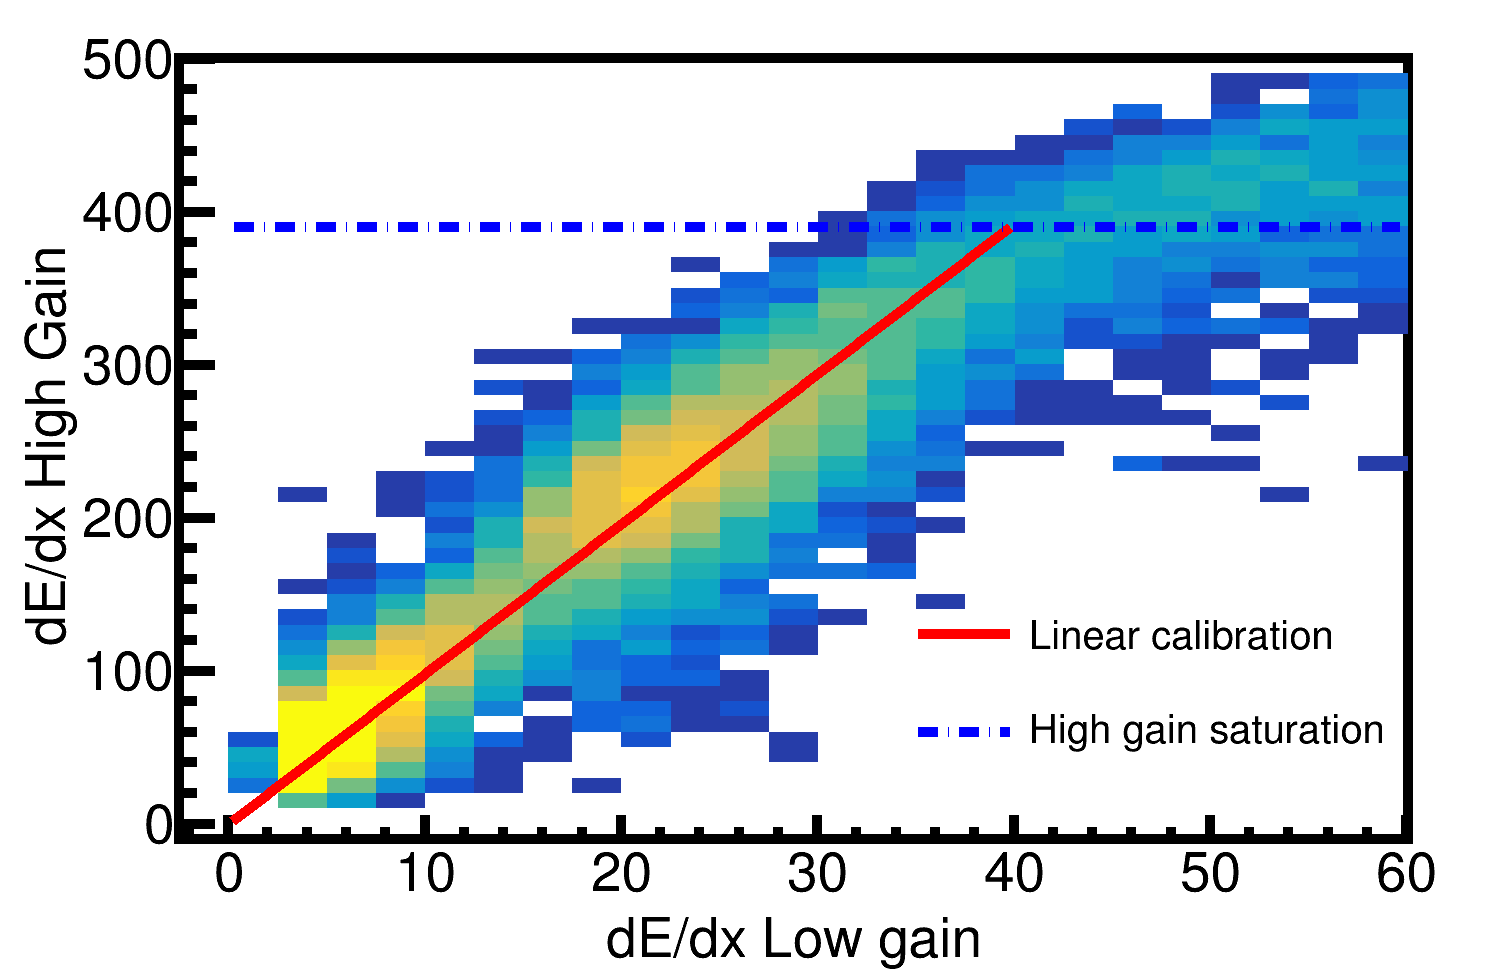
\includegraphics[width=\linewidth]{highlowcal.png}
\caption{Calibration of low high.}
\label{fig:highlowcal}
\end{figure}

Figure~\ref{fig:highlowcal} shows the correlation plot of $\langle dE/dx\angle$ of the high versus the low gain sections. The effects of the high gain channel saturation can around a value of 400 ADC\si{\per\milli\metre} and plateaus, where as the low gain does not. A linear fit was performed for the calibration  between the high gain channel $h_c = G\cdot l_c$, where $l_c$ is the value of the low gain channel and $G$ is the gain factor. In the case where the low anode voltage was \SI{1214}{\volt}, the gain factor was 9.8 where as in the case of \SI{1085}{\volt}, the gain factor was ???.  The calibration factor was applied inside of the decoder task. A map of the channels which are impacted by the low anode wire voltages and the relevant gain was input into the software. In the decoder task the raw ADC spectra was multiplied by the input gain for a given channel. The thresholds of those channels also were multiplied by the same factor since the noise levels were also artificially magnified by the same gain factor. 

\subsection{Extending the dynamic range of the Electronics}
Using a TPC for measurements of HIC in nuclear physics presents a different set of challenges as opposed to higher energy experiments. Typically in higher energy experiments the charge of particles is Z$e$, where Z=1. Also, the particles are traveling at higher energies in which the energy losses are near or close to the minimum in the energy loss curve. The dynamic range of electronics in such experiments can cover a wide range of particle energies in the energy loss curve. In nuclear HICs, we are interested in measured particles ranging from Z=1-3 resulting from the collision, and even higher in some applications. As seen in Eq.~\ref{eq:bb}, the energy loss is proportional to $Z^2$; the energy values in nuclear HIC of intermediate beam energies (around \SI{300}{\MeVA}) in which the resulting particles are at much lower energies which are in the $1/\beta^2$ region. The energy range and particle types covered by the electronics are significantly limited by the dynamic range limitations of the electronics as the charge of a particle increases and the velocity decreases. 

Several TPCs have tried to address this issue by having regions of low and high gain, either in amplification gain or in electronics gain. Here we run into the issue that high velocity particles will have little to no signal in the low gain regions. At lower velocities, particles will deposit much charge over the low gain regions but will saturate the high gain regions, whose charge values are usually lost. Only within the dynamic range will tracks have the best momentum resolution, outside the dynamic range clusters will be missing in the sections which depend on the track velocity, lowering the momentum resolution of tracking. There are ongoing efforts in the nuclear community to develop new electronics which hope to mitigate these persistent issues in TPC electronics CITE HERE, by being able to switch to a lower gain value when the maximum range is reached. Though, it is quite useful to develop a software technique which may extend the dynamic range of TPC electronics without the use of external hardware, especially in experiments which have already been performed with preexisting electronics technologies. 

In TPCs, the effective dynamic range can be very different from the single channel dynamic range depending on the application. Typically TPCs are operated inside of a magnetic field for reconstructing momentum of each particle, which requires sub-millimeter precision in the position determination of the track path. This is achieved by averaging the charge distribution over several pads. Therefore the effective dynamic range is related to the relative charge values of adjacent pads (between the center pad and outside pads). For example, to measure minimum ionizing particles the signal to noise ratio of the pad with the smallest charge in the distribution should be some reasonable value above noise, say at least 6:1 signal-to-noise ratio (SNR). From Section \ref{sec:prf}, we know the central pad in the cluster holds 80\% of the total charge, where as the two adjacent pads each hold the remaining 10\%. If we require the adjacent pads to have a SNR of 6:1, then the central pad would have a SNR of 50:1. Considering this is the SNR for minimum ionizing particles, and the maximum SNR in a channel is 800:1, this means the effective dynamic range in the TPC is roughly 16 times that of minimum ionizing particles, if we intend to have adequate position and tracking resolution. 

The dashed lines and vertical blue bar in Fig.~ \ref{fig:intro} are separated by a factor of 20, representing the typical effective dynamic range in a TPC. This dynamic range estimate should be regarded as approximate because the energy loss fluctuates significantly about the most probable energy loss, with a long ``Landau'' like tail, as described by Bichsel \cite{bichsel}. Nevertheless, the blue dashed lines and vertical blue bar illustrate that the range of energy losses sampled in a fixed gain readout system is limited. One can change the gain and shift the energy loss range that can be sampled, but the dynamic range itself cannot be increased.

  
\begin{figure}[ht!]
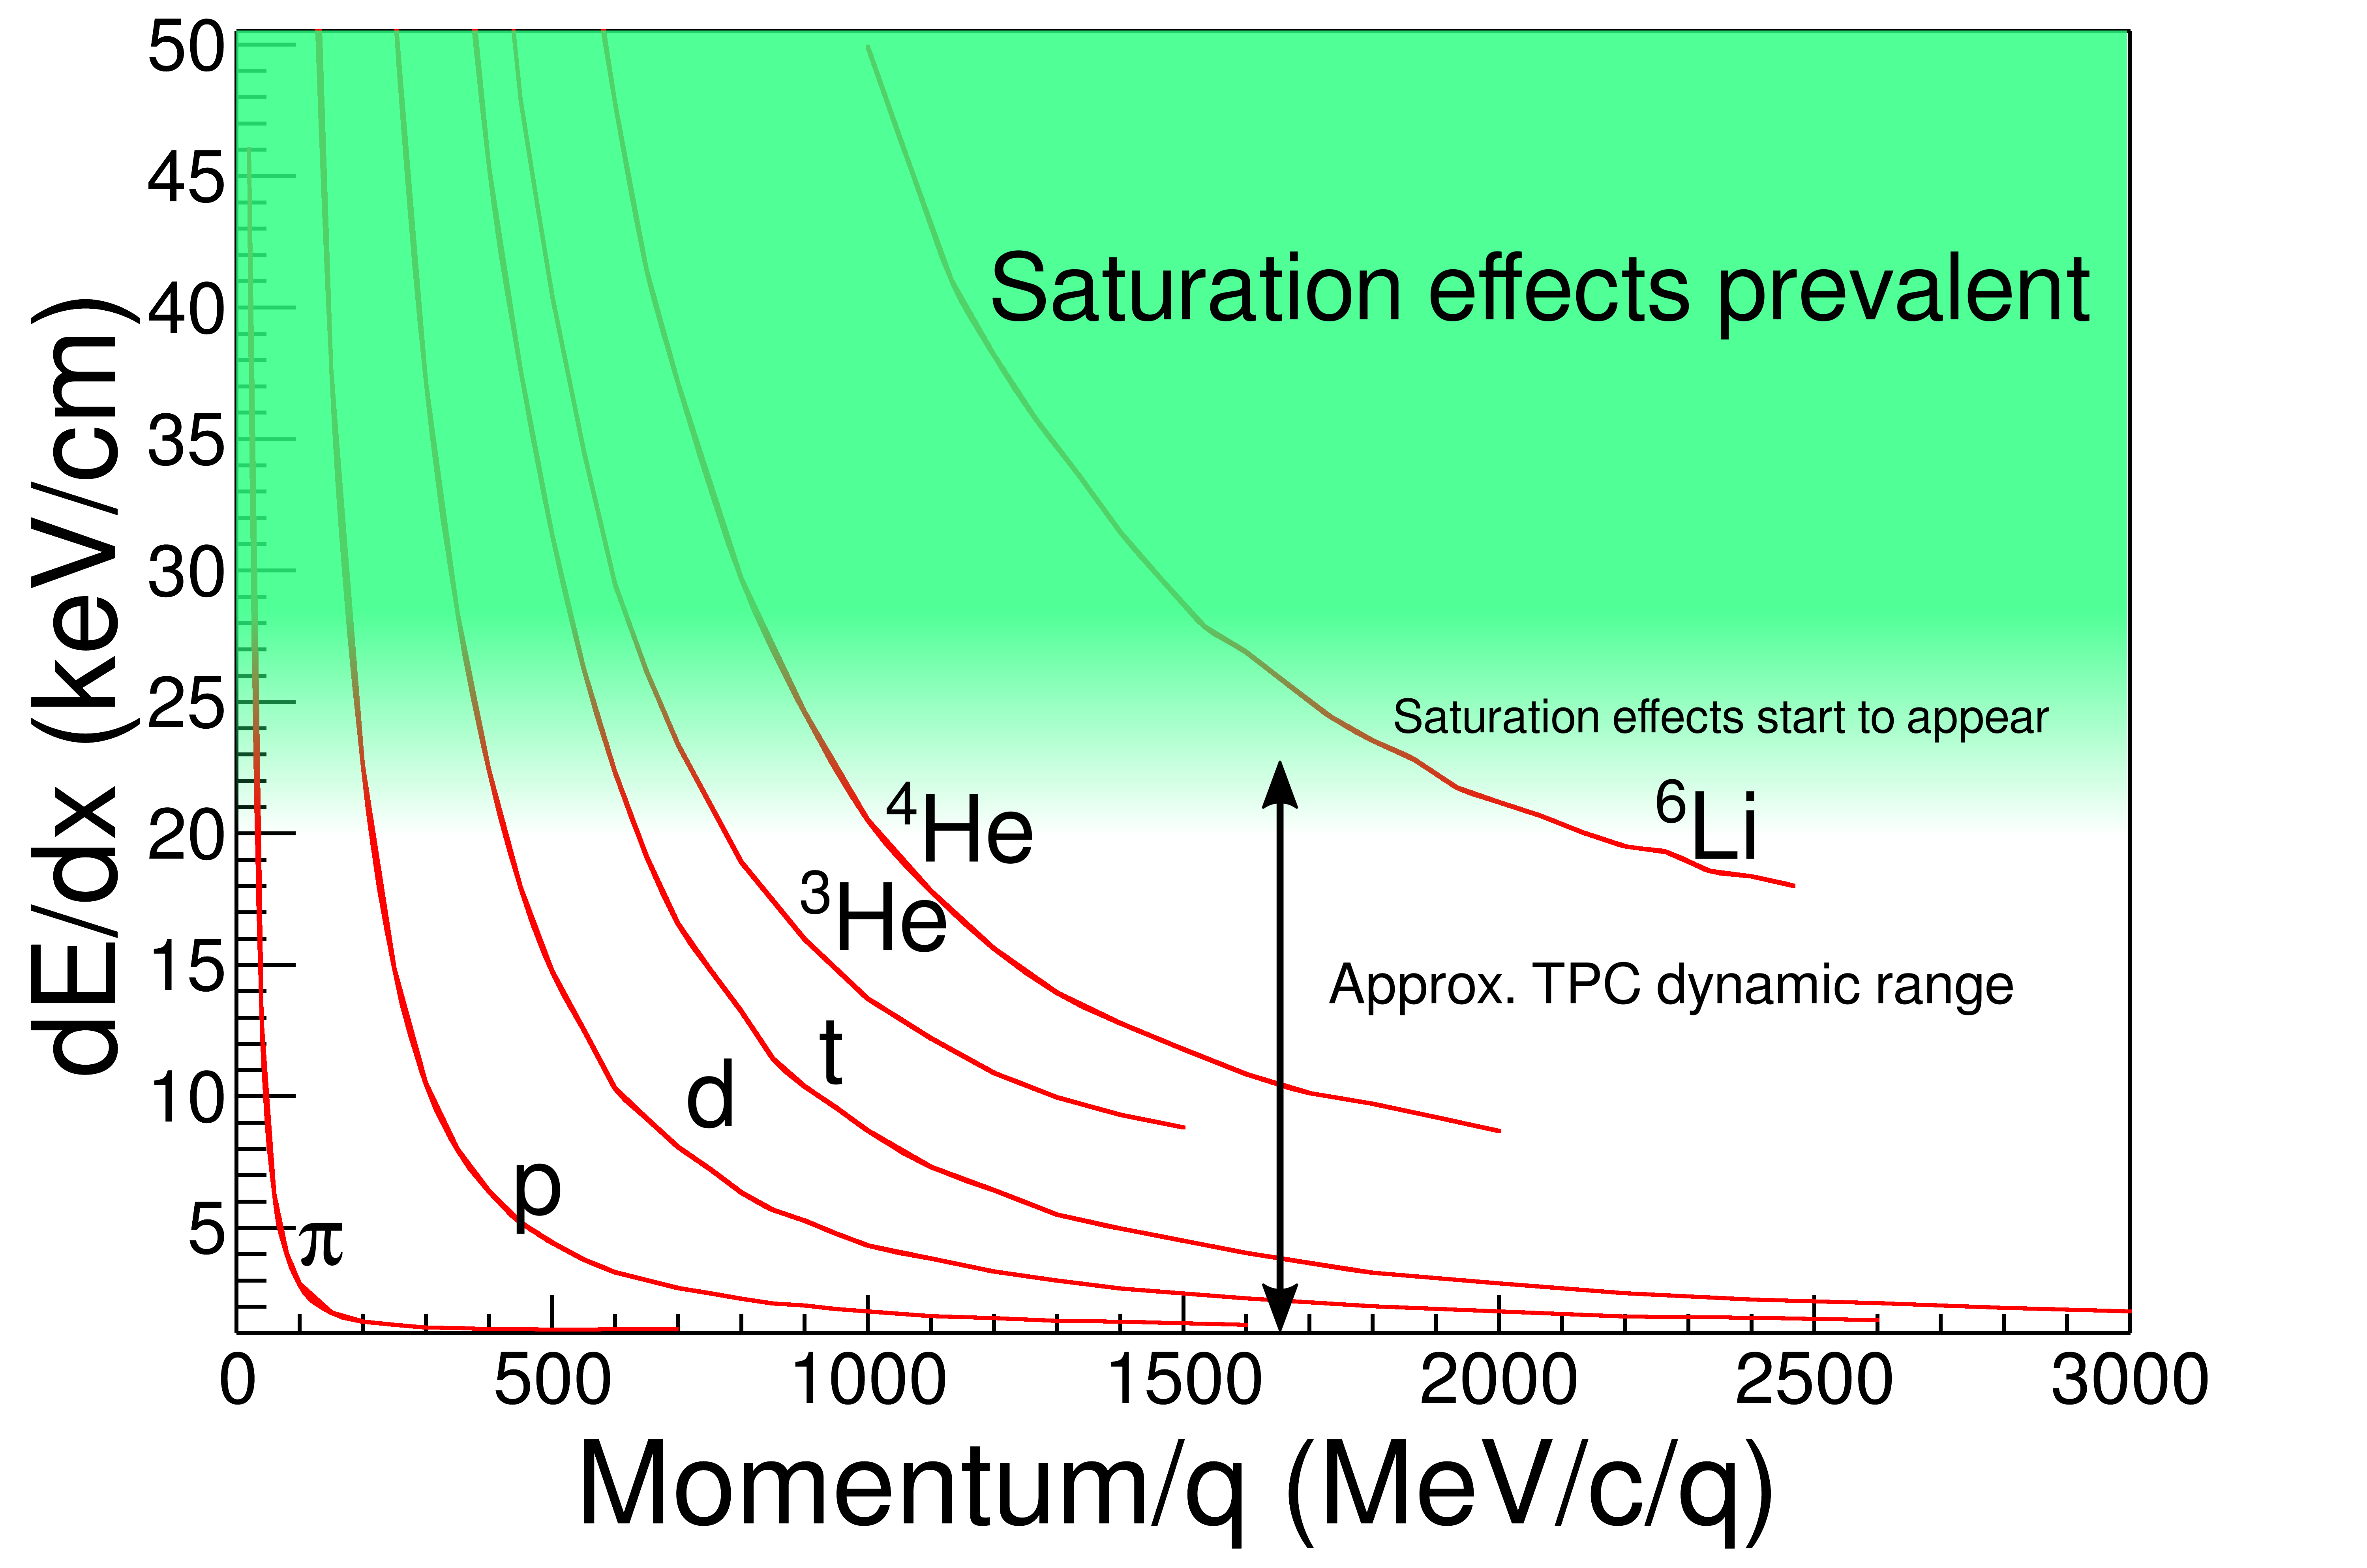
\includegraphics[width=\linewidth]{intrographic}
%\includegraphics[width=\linewidth]{intrographic_2}
\caption{The expected $dE/dx$ lines of different particles are given in red as calculated by Geant4. The approximate dynamic range of the TPC is shown by the vertical bar for the gain setting used in the experiment. Anything outside of this region would be saturated to some degree.}
\label{fig:intro}
\end{figure}

The rapid increase in the stopping powers at low momentum illustrates the degree to which the effective dynamic range can be exceeded and highlights the problems encountered in studies of intermediate HICs, in which light particles with low momenta are abundantly produced along with highly charged particles. Similar problems are encountered when TPCs are used as active targets in direct reaction studies with rare isotope beams \cite{pattpc}. Several techniques have been employed to increase the observable range of energy losses; typically by lowering the electronics gain of selected readout channels, or by changing the gas amplification at the readout plane in certain areas of the TPC \cref{eos,pattpc}. The results of changing the gas-gain, or the electronics gain, are rather similar in that reducing the gain to sample a range of higher energy loss makes the TPC effectively blind to minimum ionizing particles in  the regions of lower gain.


\subsection{Experimental Pad Response Function}

The pad response function of the TPC was extracted from non-saturating hits and clusters in tracks at various track crossing angles. As in Fig.~\ref{fig:topview}, we postulate that the PRF is a function of the total charge deposited in a cluster $Q = \sum_i q_i$, and the difference in position of the center of the $i^{th}$ pad, $x_i$, to the mean position $\bar{x} = \sum_i x_i q_i/Q$, defined as $\lambda_i = x_i-\bar{x}$. The PRF is simply defined as the charge fraction of each pad as a function of $\lambda$, as shown in Equation \ref{eq:prf}. 

\begin{equation}\label{eq:prf}
PRF(\lambda_i) = \frac{q_i(\lambda_i)}{Q}
\end{equation}

Averaging over many events in the experimental data, the resulting PRF for the S$\pi$RIT TPC is shown in Fig.~\ref{fig:expprf}. Here we see the deviations from the expected analytic Gatti distribution (black curve), whereas fitting with a two parameter Gaussian function (red curve) gives a better description of the  data, Eq.~\ref{eq:gaus}, with the two parameters being the normalization coefficient, $N_0$, width $\sigma$, and with a mean value assumed to be 0.

\begin{equation}\label{eq:gaus}
PRF_{\mathrm{Gaus}}(\lambda) = N_0 e^\frac{-\lambda^2}{2\sigma^2}
\end{equation}

\begin{comment}
\begin{figure}[ht!]s
\begin{overpic}[width=\linewidth]{fig5.pdf}
\put(61,55){\contour{white}{ PRF${}_{\mathrm{Gaus}}(\lambda)$ eq. \ref{eq:gaus}  }}
\put(61,49){\contour{white}{ PRF${}_{\mathrm{Gatti}}(\lambda)$ eq. \ref{eq:gatti} }}
\end{overpic}
\caption{Experimental pad response function of many events for a crossing angle of $85^{\circ} < \theta \leq 90^{\circ}$.  }
\label{fig:expprf}
\end{figure}
\end{comment}


The shape of the PRF depends on the crossing angle of the track \cite{gatti}, which determines how wide the charge is distributed along the wire. Figure~\ref{fig:prfpimData} shows the PRF of $\pi^-$ tracks versus the crossing angle $\theta$ of the track. The PRF gets wider starting from $90^{\circ}$  and until where we switch clustering directions at $\ang{45}$; if we did not switch clustering directions the PRF would become wider until it was a uniform distribution and there was no position resolution. Switching from $x$ to the $z$ direction clustering the opposite trend is seen where the PRF becomes narrower  going from $45^{\circ}$ to $0^{\circ}$, as the position resolution gets better.




\begin{figure}[!htb]
     \centering
	 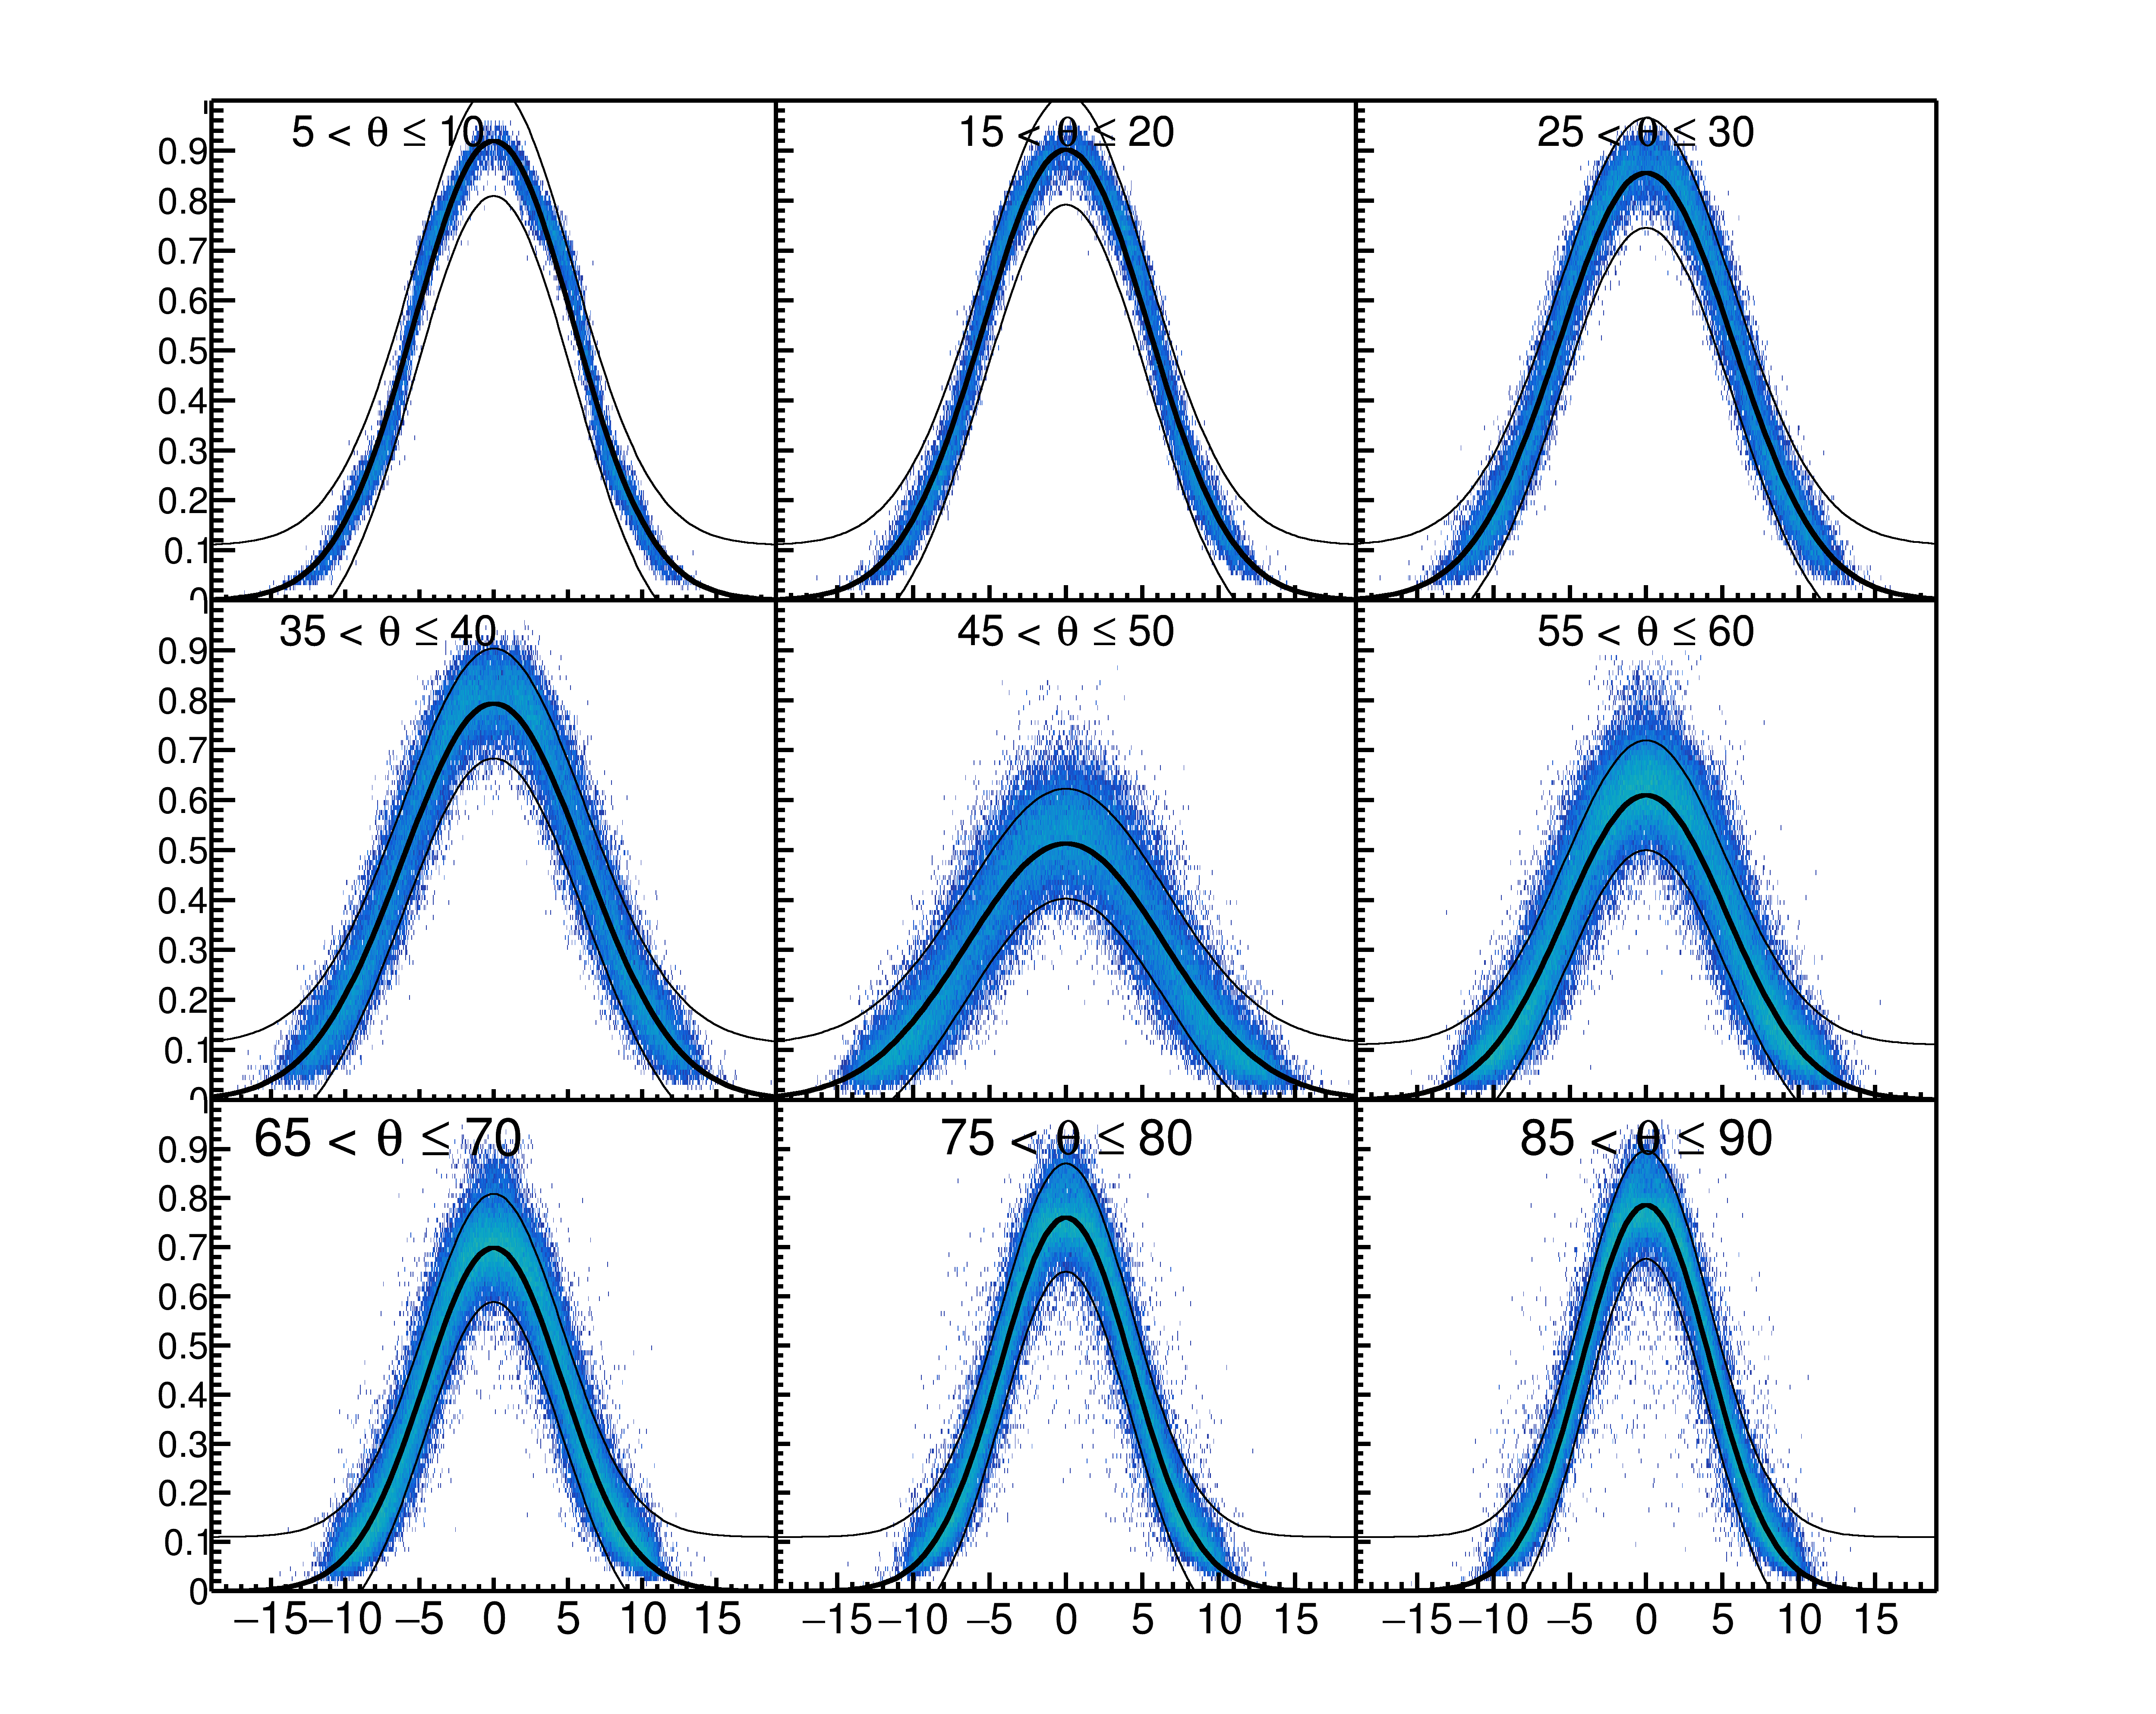
\includegraphics[width=\textwidth]{PRFs_data_wcut.png}
     \caption{PRF response from $\pi^-$ data. }
     \label{fig:prfpimData}
\end{figure}

\begin{figure}[ht!]
\vspace{5mm}
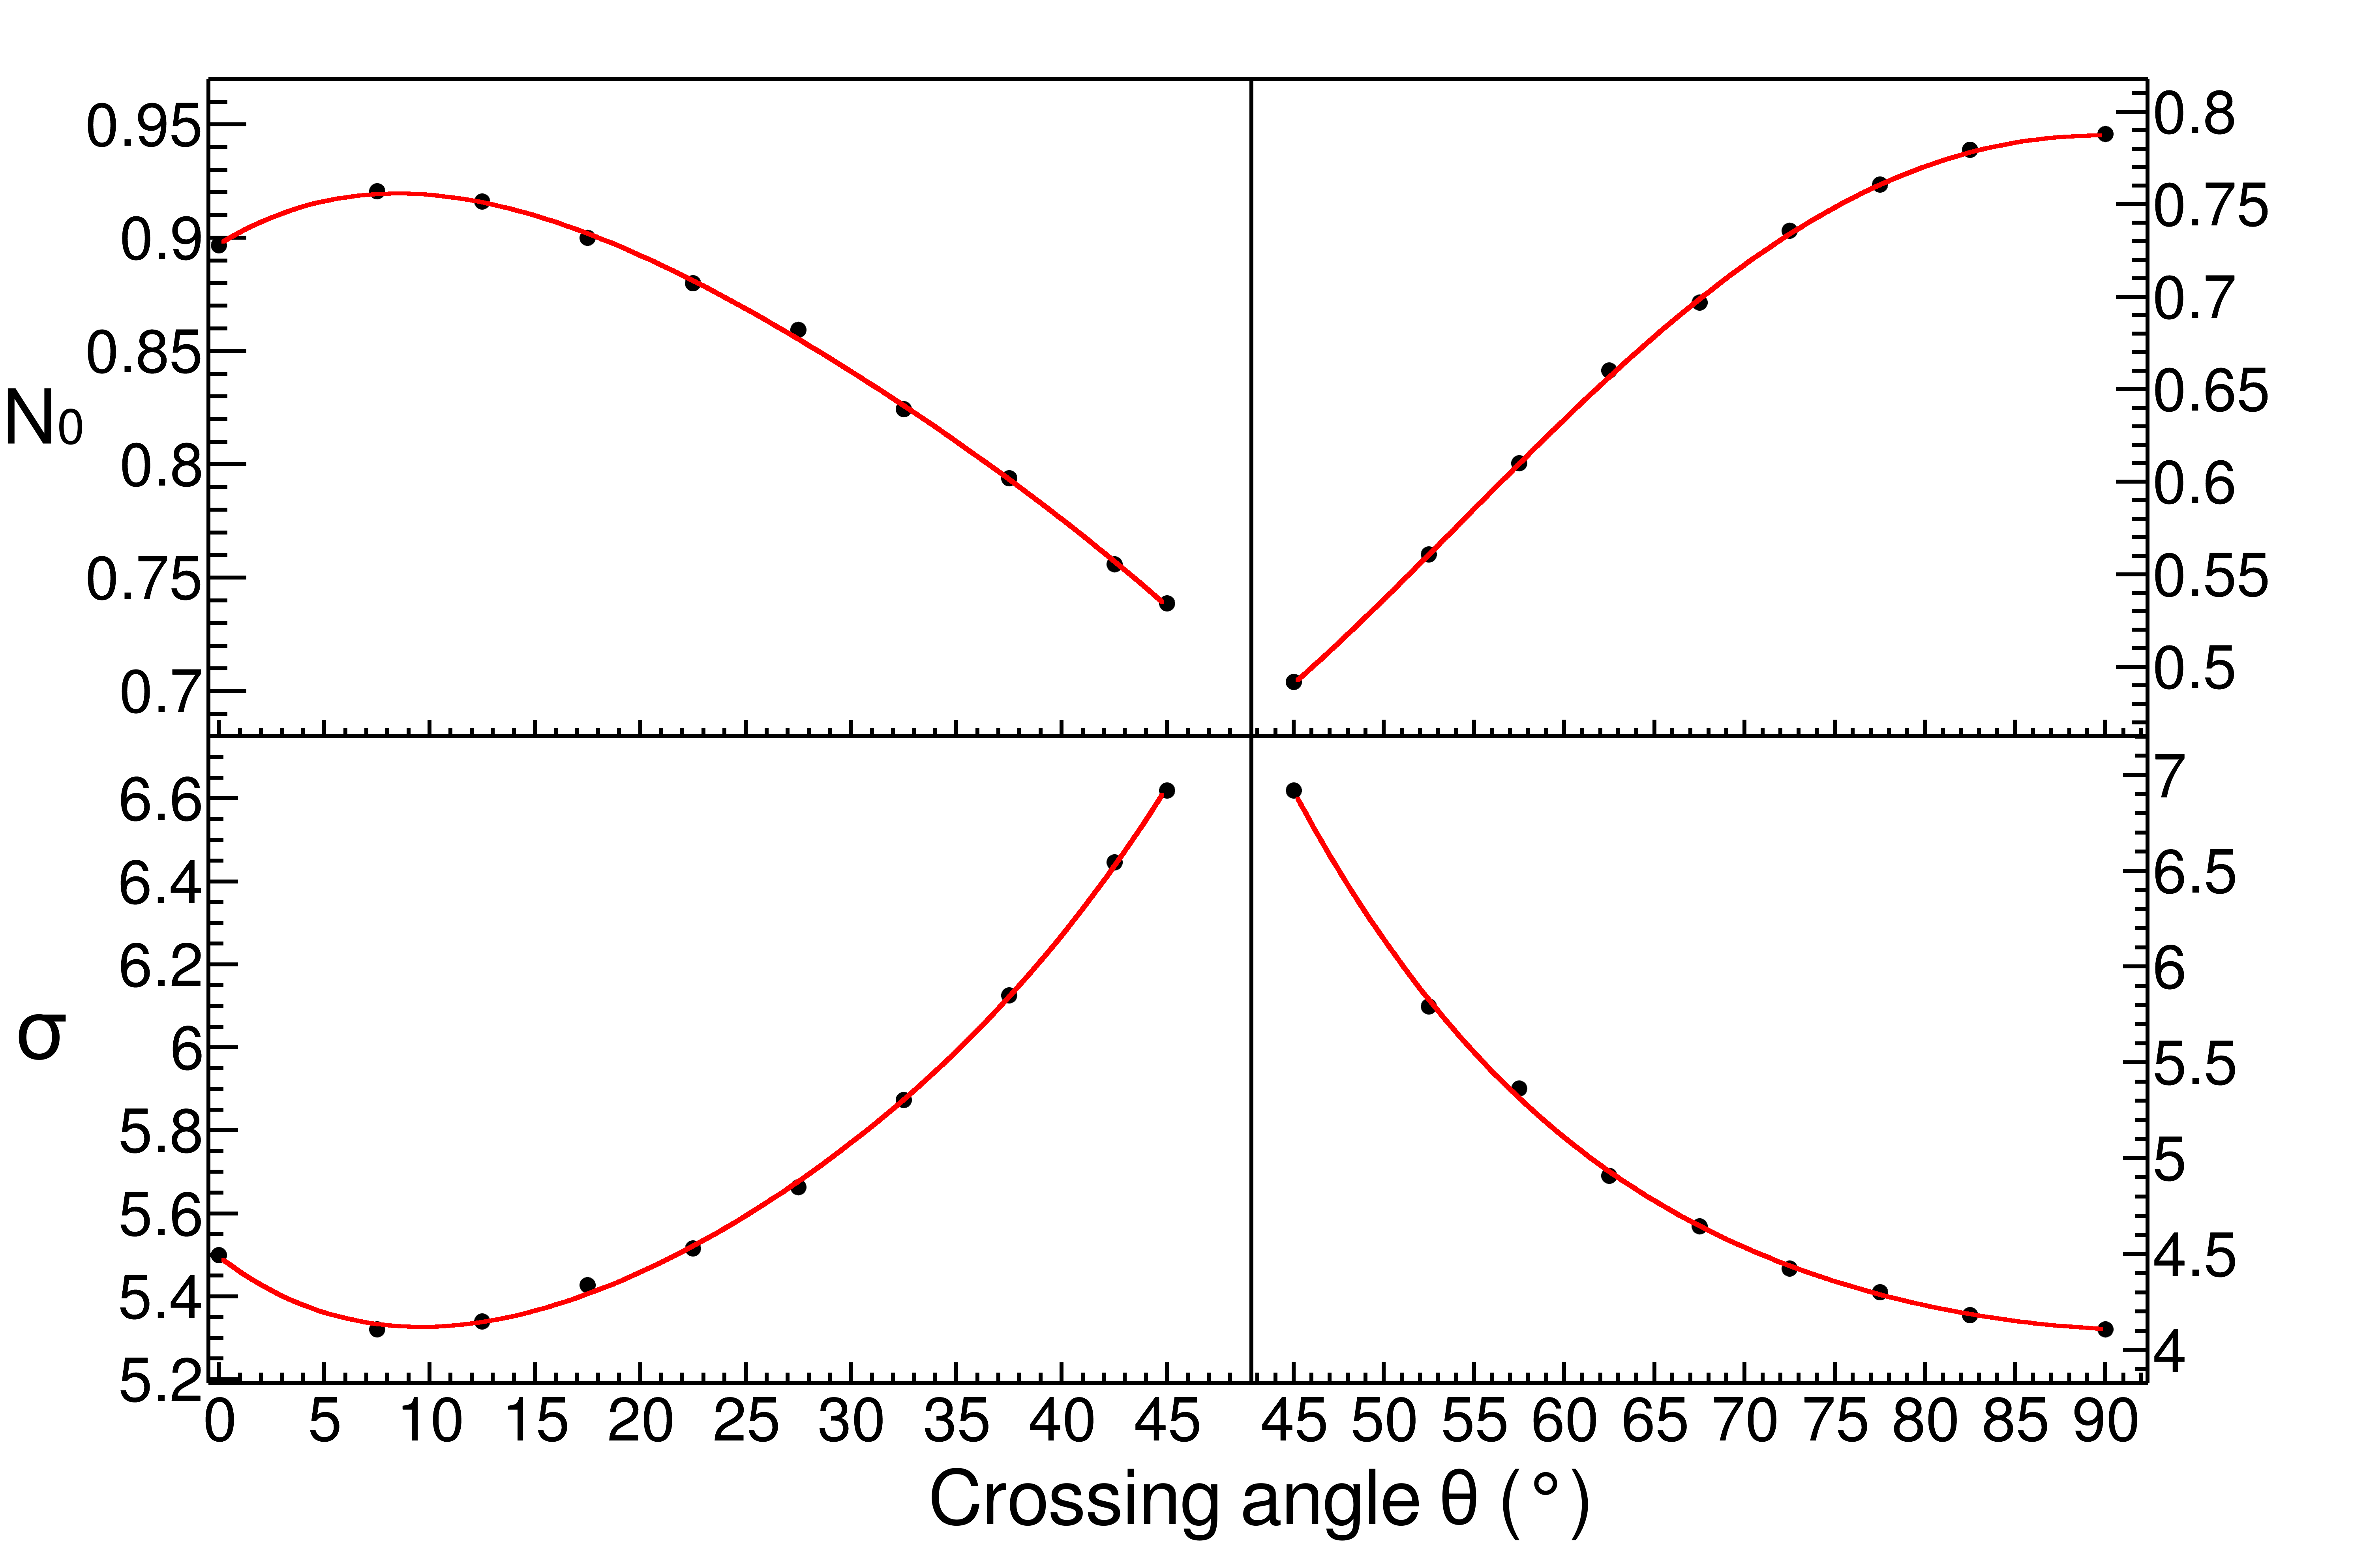
\includegraphics[width=\linewidth]{fig7}
\caption{Parameters $N_{0}$ and $\sigma$ as a function of the crossing angle $\theta$ with the $4^{th}$ order polynomial fits.}
\label{fig:normsigma}
\end{figure}

\begin{comment}
\begin{table}
\centering
 \begin{tabular}{||c c c c c c||} 
 \hline
 Coefficient & $c_0$ & $c_1$ & $c_2$ & $c_3$ & $c_4$ \\ [0.5ex] 
 \hline\hline
 $0 < \theta < 45$ & & & & &  \\ [.25ex]
 \hline
 $N_0$ & .897 & 5.766E-3 & -4.263E-4 & 7.444E-6 & 5.705E-8 \\ 
 \hline
 $\sigma$ & 5.496 & -3.920E-2 & 2.693E-3 & -5.208E-5 & 5.334E-7\\
 \hline
 $45 < \theta < 90$ & & & &  & \\ [.25ex]
 \hline	
 $N_0$ & 1.220 & -6.258E-2 & 1.608E-3 & -1.492E-5  & 4.654E-8 \\
 \hline
 $\sigma$ & 31.368 & -1.109 & 1.779E-2 & -1.336E-4 & 3.940E-7\\
 \hline
\end{tabular}
\caption{Coefficients of the $4_th$ order polynomial fit to the Gaussian parameters $N_0$ and $\sigma$. The polynomial form is given as $c_0 + c_1 x + c_2 x^2 + c_3 x^3 + c_4 x^4$}
\label{tb:coeff}
\end{table}
\end{comment}
 
A Gaussian fit was performed were performed to the experimental data with  $\ang{5}$ width bins from $\ang{0} < \theta \leq \ang{90}$. Figure~\ref{fig:normsigma} shows the two parameters resulting from fitting the the Gaussian function given in Eq.~\ref{eq:prfgaus} are plotted versus $\theta$. A $4^{th}$ order polynomial fit of these parameters allowed for interpolating for any given $\theta$ value as seen by the black line. 


\subsection{Method of Desaturation}
\label{sec:desat}

\begin{figure}[ht!]
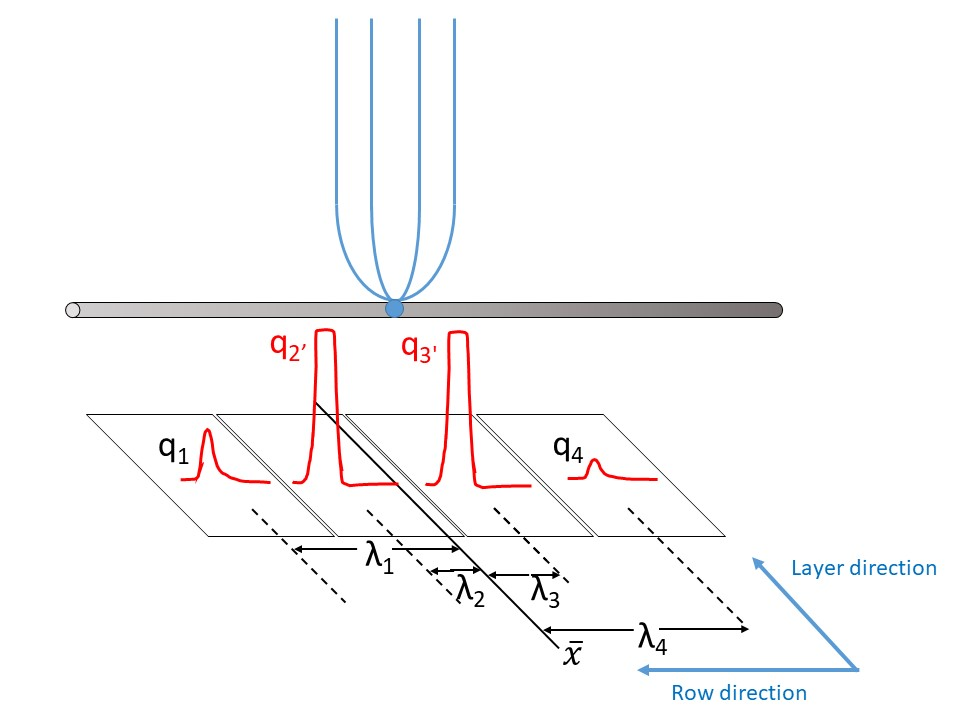
\includegraphics[width=\linewidth]{saturated_pads}
\caption{A typical case of a saturating event. The red pulses represent the time bucket signal for each collected charge. The pads directly underneath the avalanche point, $q_{2'}$ and $q_{3'}$, are saturated while pads farther away, $q_1$ and $q_4$ are not saturated.}
\label{fig:satpad}
\end{figure}


We will use the term ``desaturation'' to describe the process of correcting the charge values of the saturated pads. Figure~\ref{fig:satpad} shows a typical situation of saturated signals in a given cluster of hits. When an avalanche causes a large enough induced signal, it is the pads directly underneath which collect the largest charge becoming saturated; denoted here as $q_{2\textprime}$ and $q_{3\textprime}$. Pads further away collect less charge and typically are not saturated; the non-saturated pads are detonated here as $q_{1}$ and $q_{4}$. Though the true charge value in the saturated channels are lost, we know that the distribution of all charges must follow the PRF which is a fixed feature of all TPCs, and has been experimentally measured above. From the tracking information, we know a given clusters crossing angle and can interpolate to get the corresponding parameters for the PRF described in Fig.~\ref{fig:normsigma}.

We assume the distance of each pad to the track, $\lambda_i$, is fixed, defining the fraction of charge each pad receives as given by the $PRF(\lambda_i)$ function. To determine the best estimate for the charge values of each saturated pad, a chi squared function is minimized,

\begin{equation}\label{eq:chi}
\chi^2 = \sum_i \frac{(q_i^{\mathrm{obs}} - q_i^{\mathrm{expect}})^2}{q_i^{\mathrm{expect}}},
\end{equation}


where $q_i^{\mathrm{obs}}$ are the non-saturated charges and $q_i^{\mathrm{expect}}$ are the charge values expected from the PRF calculated as $q_i^{\mathrm{expected}} = Q\cdot PRF(\lambda_i)$. The saturated charge values $q_{i}^{\textprime}$ are treated as unknown variables and are allowed to vary in the $\chi^2$ minimization; the values calculated by the minimizer are added to the total expected charge $Q$. 


\begin{figure*}[t]
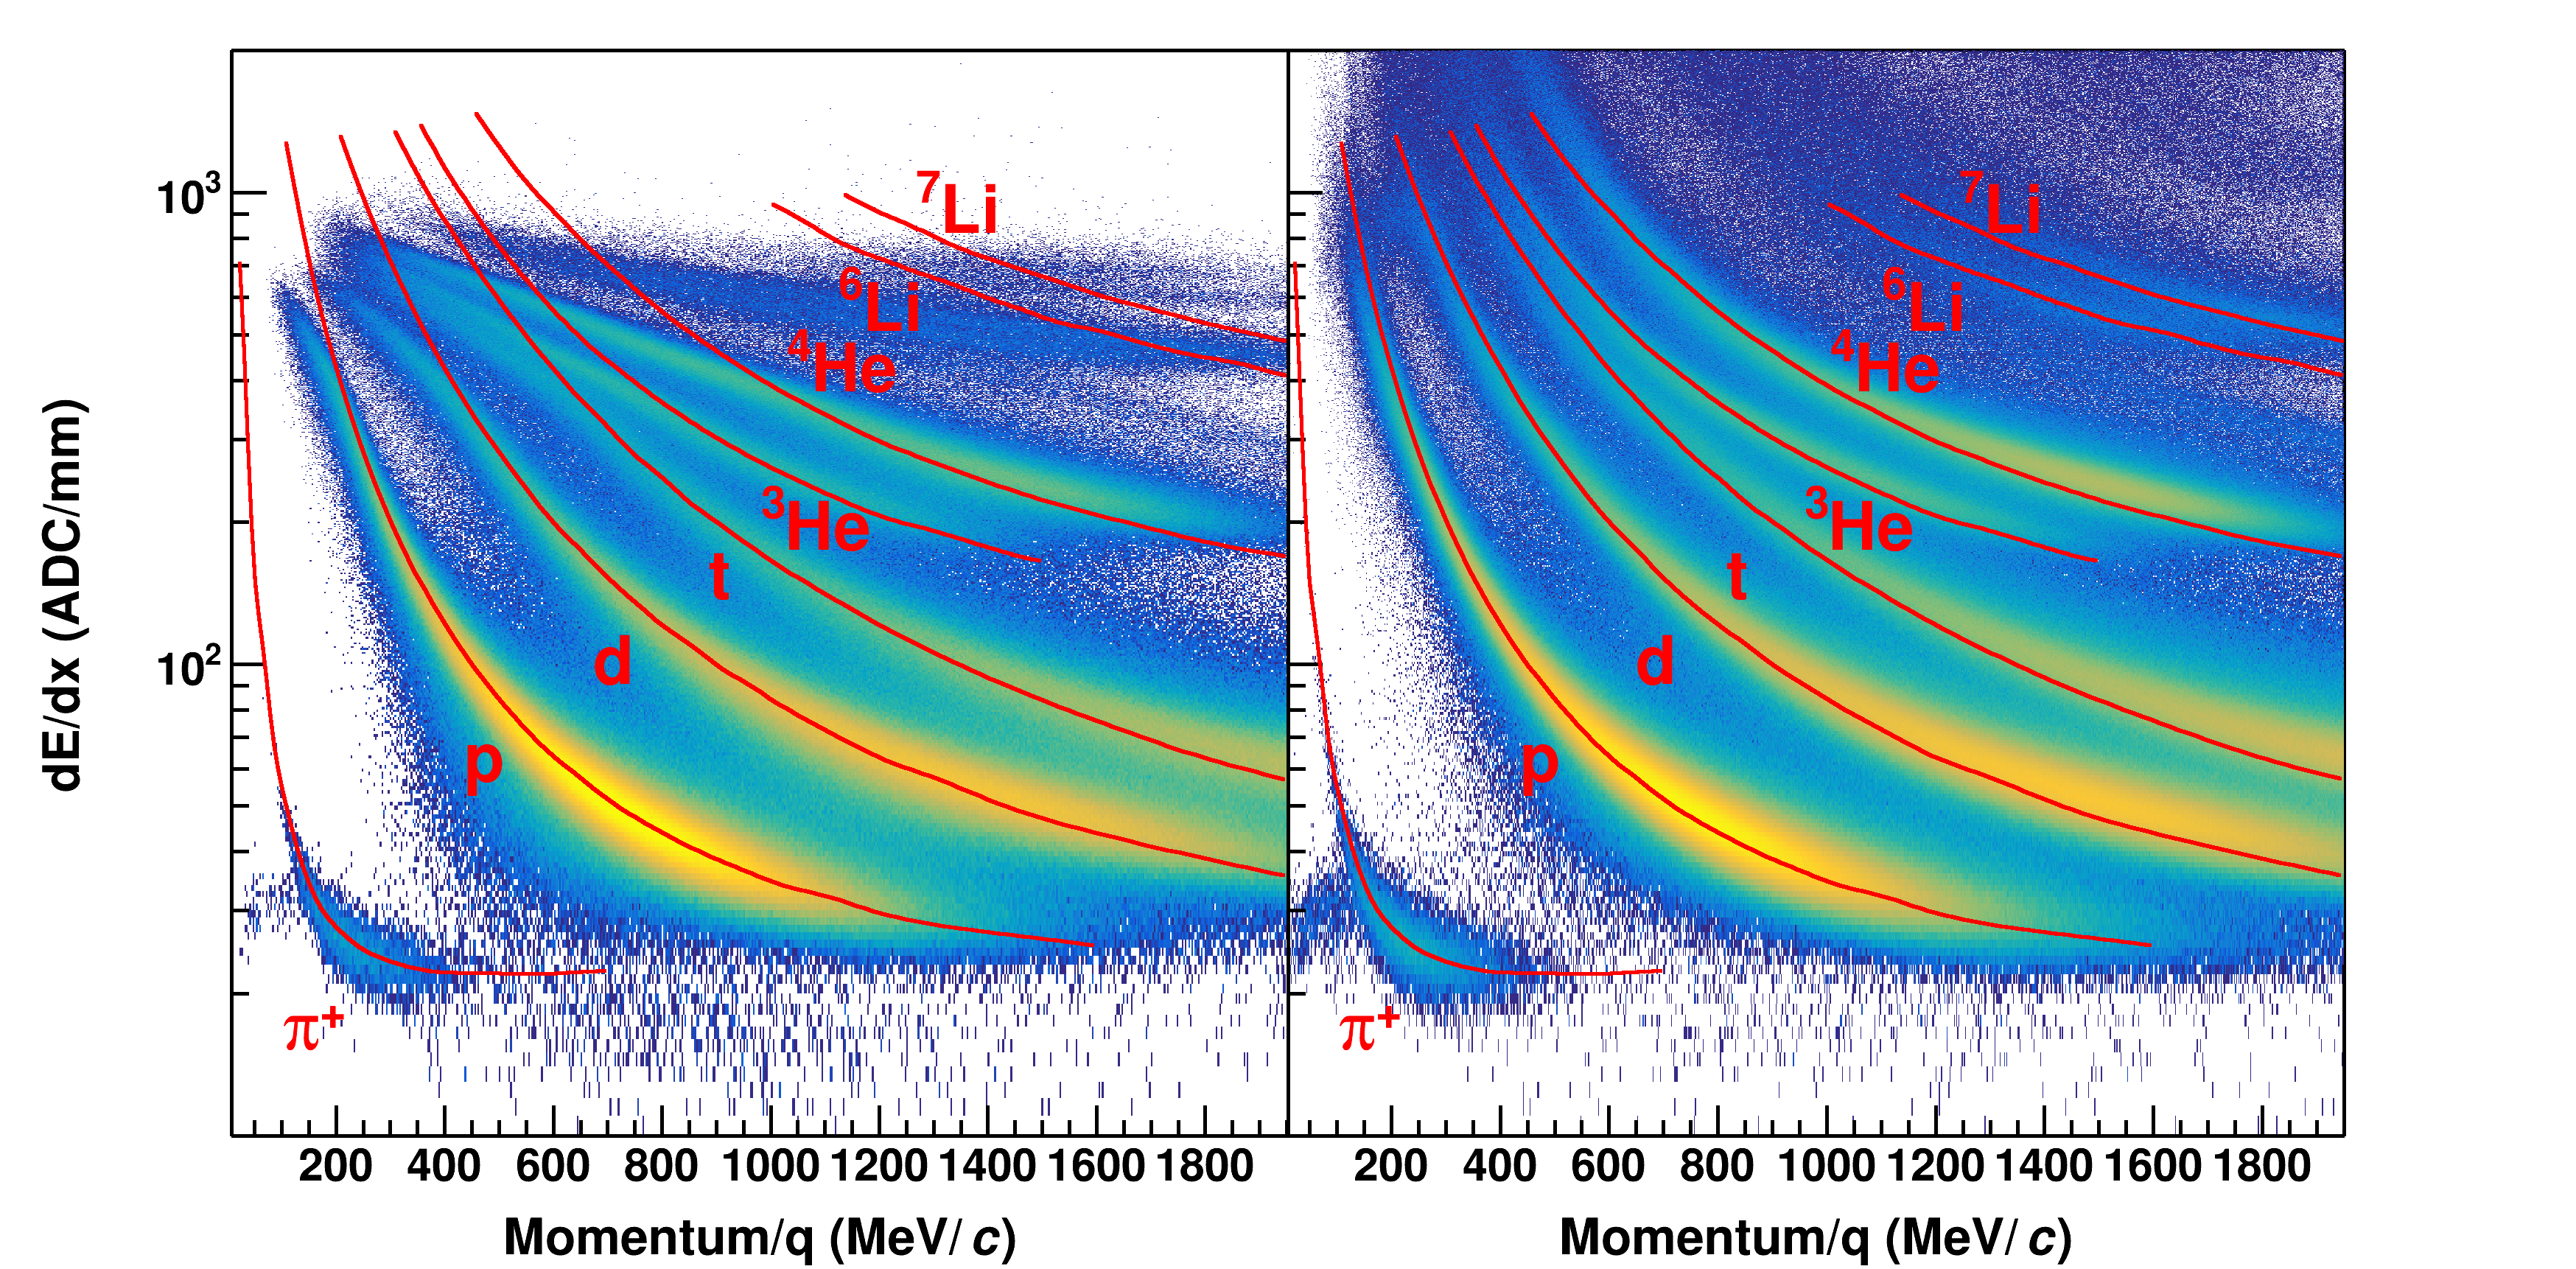
\includegraphics[width=\linewidth]{data_combine}
\caption{Uncorrected (left panel) and desaturated (right panel) collision data at polar angles of $\theta < 40^{\circ}$ and azimuthal angles between $-80^{\circ} < \phi < 80^{\circ}$}
\label{fig:data_combine}
\end{figure*}

Tracks which saturate pads in the high anode wire voltage region are not saturated in the low anode voltage region. By comparing the $\langle dE/dx\rangle$ values of these two sections, we can directly measure the success of the desaturation in the high gain regions. While this desaturation technique avoids the need to lower the gain of any region, the low anode voltage region proved to be a direct measurement of the success of this technique.
 
Figure~\ref{fig:lowvshigh} shows the the $\langle dE/dx\rangle$ values of the high gain region compared with the calibrated low gain region. The effect of saturation can be seen in the high gain region for the uncorrected data above values of 400 ADC/mm where the values plateau, where as the low gain region still returns accurate values\footnote{Un-calibrated ADC channels in arbitrary units.} Below this value the electronics are not saturated, and therefore the high and low gain sections agree. 

 After applying the desaturation method, the correlation between the high and low gain sections is restored, as seen in Fig.~\ref{fig:lowvshigh}. From this comparison, we can approximate that the correction has corrected the high gain sections to agree with low gain sections to values of 2000 ADC/mm, increasing the dynamic range by a factor of at least 5.

The success of the desaturation becomes more clear when looking at the particle identification (PID) lines. In the following PID plots the red lines represent the most probable energy loss as given by Geant4 straggling functions. A linear calibration was performed to convert keV in Geant4 to ADC in the experiment given by $ADC/mm = 19;keV/cm$.

There are pronounced PID lines of several particle species in both the uncorrected and corrected cocktail beam PID shown in the subplots of Fig.~\ref{fig:cocktail_combine}. The uncorrected data in the left panel shows the effects of saturation; the PID lines deviate from their theoretical expectations starting at around 400~ADC/mm eventually reaching a plateau. After applying the desaturation technique -- in the right panel-- we see a large improvement, most notably for the He and Li particles, which suffer the most from saturation and even ${}^{6}Li$ and ${}^{7}Li$ can be separated. A more subtle improvement of the lighter particles, (p, d, t), can also be seen in the PID lines at lower momenta.

A similar effect is seen in the experimental collision data. In Figure~\ref{fig:data_combine} though the PID suffers from more background and inefficiencies than the cocktail beam we see a similar improvement in the PID lines when comparing before -- the left panel-- and after applying desaturation -- the right panel. Notably the largest improvement is the separation of particle species at lower momenta and the separation of the Li species into ${}^{6}$Li and ${}^{7}$Li. In these regions, there was little to no PID resolution before desaturation. 

The dynamic range was extended by at least a factor of 5, as demonstrated by the improved PID lines, and quantified by direct comparison to low gain sections of the TPC. 

%Give some failures of the assumptions made

\subsection{Space Charge Corrections}
\label{sec:spacecharge}

%MAYBE ADD A LITTLE NAPKIN CALCULATION OF SPACE CHARGE TO SHOW ORDER OF EFFECT. 

As the beam passes through the field cage it ionizes the gas creating electron-ion pairs. The drift velocities of the ions are typically \SI{e4} times slower than the electron drift velocities \cite[blumrol]. Any source of ions have the potential to build up creating a positive space charge distorting the drifting electrons, biasing the track momentum. There are several regions of the TPC in which ion are created. The largest source of positive ions is created in the avalanche process near the anode wires. These ions slowly drift toward the cathode. If the gating grid is closed the ions will terminate there; though it opens occasionally  for \SI{11}{\micro\second} the ions only move \SI{1}{\micro\metre} in this time and will be captured by grid when it closes. For this reason, the source of ions resulting from the avalanche region is negligible. 

The other source of ions come from the primary ionization produced by the beam and reaction products in the detector gas. The energy loss  $\langle dE/dx\rangle \propto Z^2$, where Z is the charge of the particle type. Because the charge of the un-reacted beam is around Z~50, the ionization due to the beam is a factor of \num{2.5e3} times that of the light charged particles which mostly are of charge Z~1. It is the largest source of positive ions in the TPC. 


NEED TO PUT IN ABOUT THE GATING GRID LEAK 
 
 \begin{comment}
 
 \begin{table}[!htp] % not just 'h!'
\centering % not a center environment
\begin{tabular}{
  @{}
  l
  S[table-format=1.2]
  S[table-format=1.2]
  S[table-format=1.2]
  S[table-format=5.2]
  S[table-format=5.2]
  @{}
}
\toprule
Beam Energy Loss  &
 {${}^{132}$Sn} &
 {${}^{124}$Sn} &
 {${}^{112}$Sn} &
 {${}^{108}$Sn} &
  {Avg.}\\
  
\midrule
$\si{\kilo\eV\per\centi\meter}$ & 11.2   &.034  &5.43   &  903   &150     \\
\bottomrule
\end{tabular}

\caption{Average energy loss of each beam.}
\label{tb:beameloss}
\end{table}
\end{comment}


\begin{figure}[!htb]
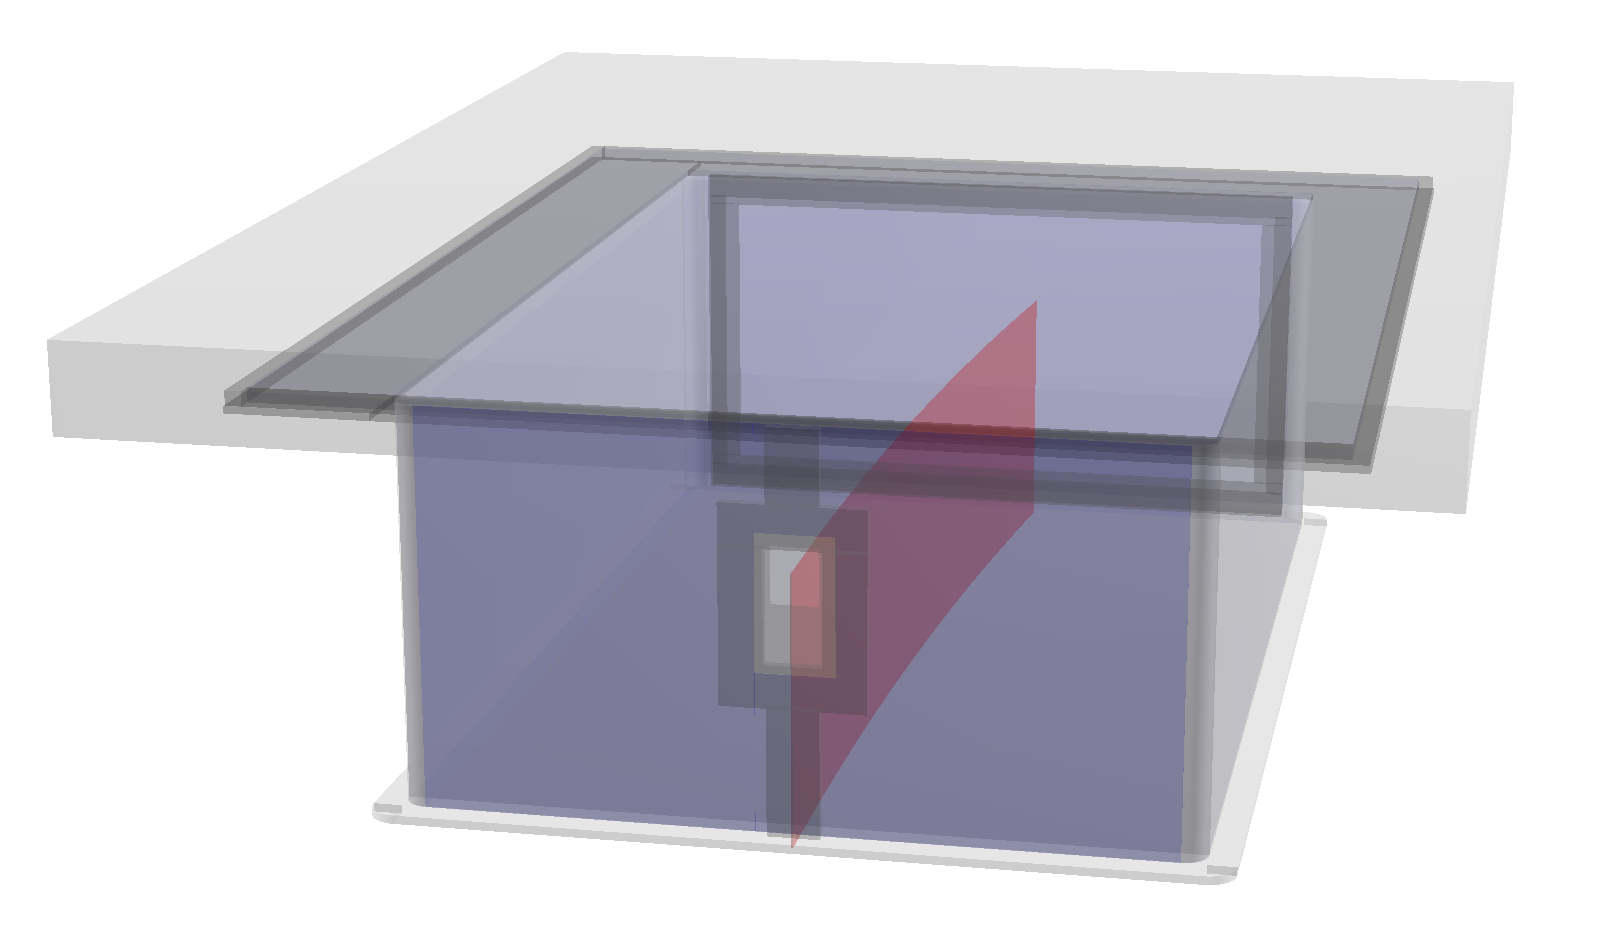
\includegraphics[width=\linewidth]{spacechg_cartoon.png}
\caption{Location of space charge in 132 Sn}
\label{fig:spacechg_cartoon}
\end{figure}


\begin{figure}[!htb]
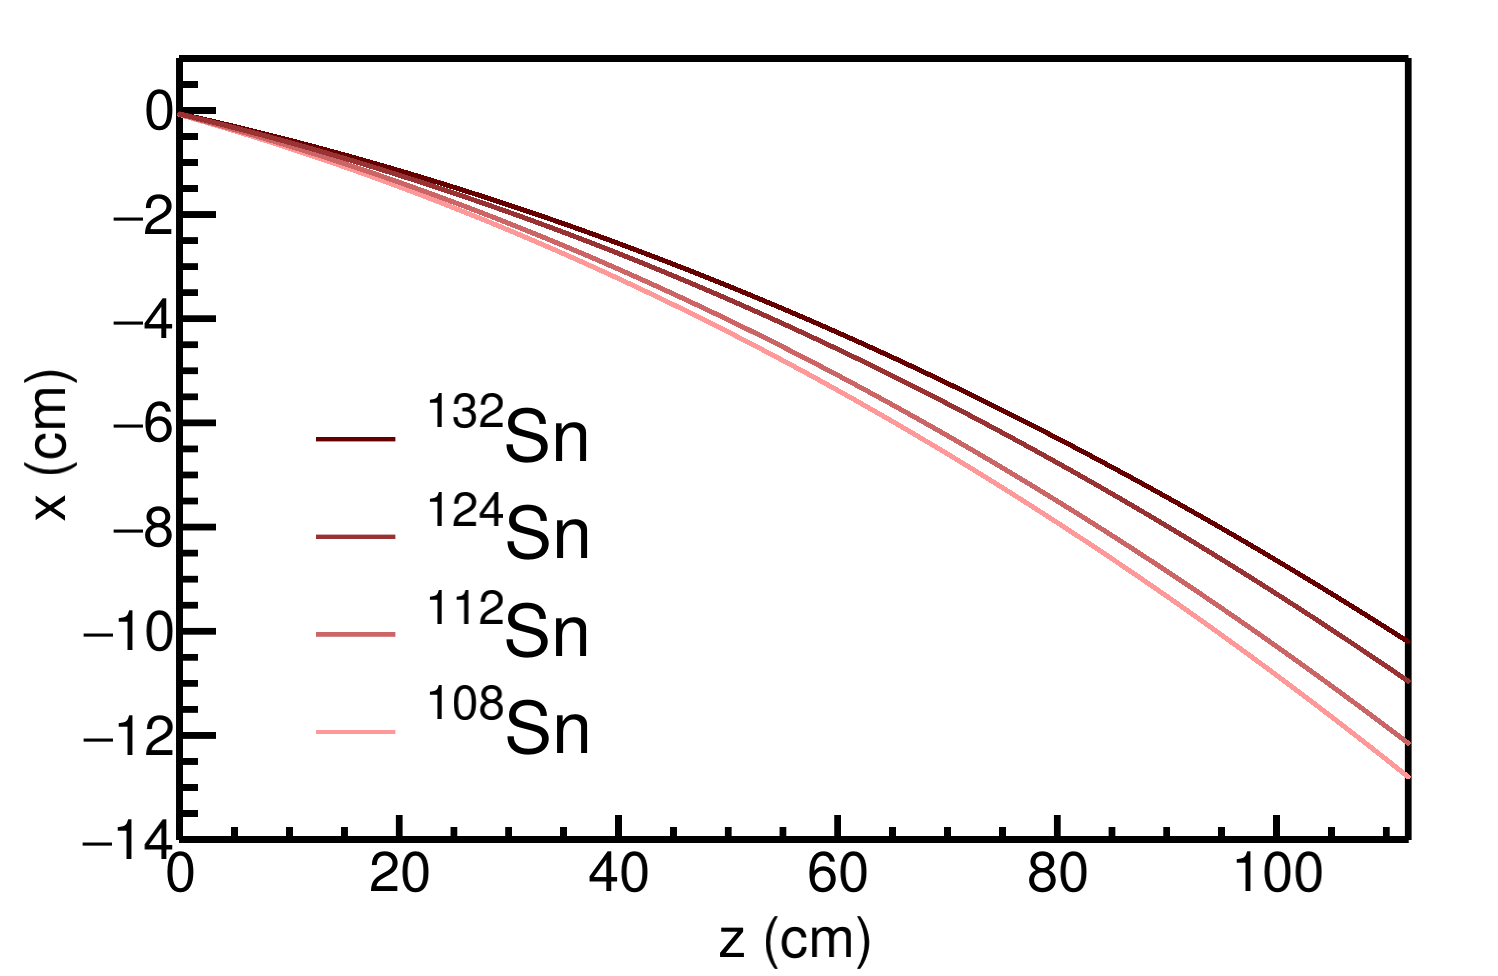
\includegraphics[width=\linewidth]{beampath.png}
\caption{Beam path of the experiments}
\label{fig:beampaths}
\end{figure}
 
 
 The beam is positioned about 25\si{\centi\metre} below the anode plane in the TPC. It takes electrons approximately 5\si{\micro\sec} to drift to the anode plane where as it takes the ions \num{5e4}\si{\micro\sec}. The beam rate in the experiment varied around a value of about 10\si{\kilo\hertz}, which has an average occurrence of 1 beam every \SI{100}{\micro\sec}; this is shorter than the time it takes for the ions to terminate on the cathode plane, resulting in a build up of positive ions. Figure~\ref{fig:spacechg_cartoon} gives an idea of the shape of the sheet of space charge carved out by the beam path. The ions from each beam create a line charge which drifts towards the cathode with a constant velocity. The average distance between sequential ion paths is about \SI{25}{\micro\metre} apart, therefore we expect the average number of beam paths that compose the sheet charge is around \num{1440} tracks -- where the distance to the cathode is \SI{29.6}{\centi\metre}. Though the arrival time of each beam track is random, the large number of tracks and small inter beam spacing allows us to approximate the sheet charge as an uniform sheet charge. 
 
 The secondary beams entering the TPC are also composed of many species of particles distributed in a finite range around the target beam. Assuming a beam of ${}^{132}$Sn were the energy loss in gas is \SI{11.2}{\kilo\electronvolt\per\centi\metre}, using the number of beams above, the conversion to electrons given in \ref{tb:gasprop}, and the beam path length of \SI{135}{\centi\metre}, the total charge density expected is \SI{3e-8}{\coulomb\per\metre\squared}. 
 

The electric potential can be calculated by solving Poisson's equation, 

\begin{equation}
\nabla^2 \phi = \rho,
\end{equation}

 where $\phi$ is the electric potential and $\rho$ is the free charge.  Since the Dirichlet boundary conditions of the field cage are defined by the cathode, walls, and pad plane, a numerical solution to the electric potential is solved through the ??? technique. The electric field is simply the gradient of the potential  $\vec{E}= -\nabla \phi$. 
 
 To reduce the need to compute a new electric field for a new value of the space charge, we notice that $\vec{E}\propto \rho$, we can therefore solve the electric field for a certain reference charge value $\rho_o$, and scale the solution for any other free charge $\rho$ by the ratio $\rho/\rho_o$. The full magnetic field map is provided by the SAMURAI collaboration \cite{magnet}. The velocity field map can be calculated from Eq.~\ref{eq:elecdrift}. The path an electron drifts through this velocity map is propagated by using a time stepped $\mathrm{4}^{\mathrm{th}}$-Order Runge-Kutta integration from a given starting point of the electron. We do not add details of the electric field around the anode wires which is only relevant for the small gap between the ground and anode plane. Over this small gap the space charge corrections have very little effect. 
 
 The correction map is calculated by starting from the anode y-position and the measured position on the pad-plane (x,z), and stepping backward in time in the Runge-Kutta integration through the velocity field map until the electron reaches the measured y-position, which is split into a grid that fills the 3-dimensional volume of the field cage. 
 
 The correction is handled within the STCorrection task in the software. A data base of the sheet charge values for every run is read in and the electric field is calculated for the reference charge for a given beam path. The electric field and velocity map is scaled by the ratio of the space charge in the particular run and the reference run $\rho/\rho_o$ and the correction map is calculated. The measured clusters value (x,y,z) position is input into the correction map which interpolates and outputs the correction values $dx$ and $dz$ which correspond to that cluster. The cluster position is shifted to new positions $x\textprime = x + dx$ and $z\textprime = z + dz$, before going on to the momentum and vertex finding algorithms.  
 
 It has been shown before that the amount of space charge present in the chamber is related to observables such as the distance of closest approach of each track to the vertex point \cite{starSC}. In the presence of no space charge, you would correctly expect the distance of closest approach of each track to the vertex point would be a distribution centered around the true vertex location. Since the tracks are distorted by the space charge, which affects different regions of the TPC differently, a bias is introduced to the measured vertex location and widens the distribution to vertex of each track.  

An example of the distortion map in the TPC is shown in Fig.~\ref{fig:sc_shift} with left-going tracks shown in blue, and right-going tracks shown in green; the vectors show the direction of distortion and their magnitude have been magnified by ??? times to show the detail. The dashed lines show the effects the track shifted due to the space charge map where left and right-going tracks are affected differently. Right-going tracks tend to higher momentum values and the left-going tracks going to lower momentum values, for positively charged particles. 

\begin{figure}[!htb]
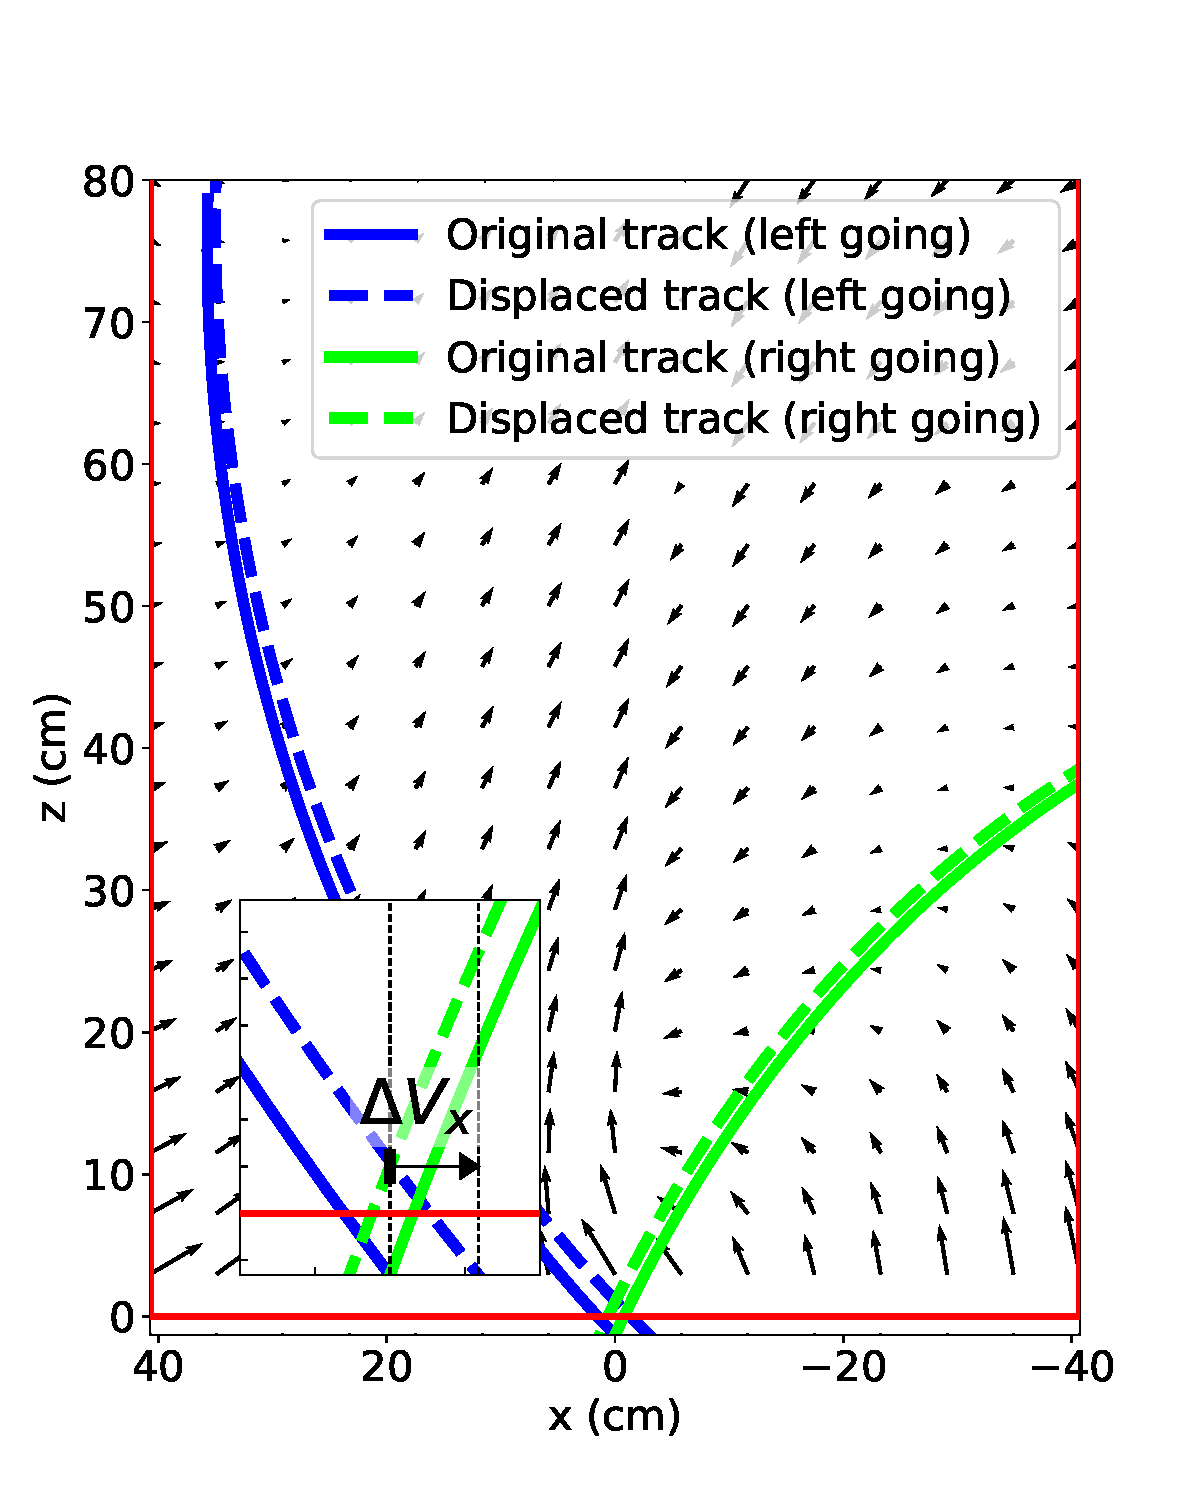
\includegraphics[width=\linewidth]{Effect_SC.pdf}
\caption{Shift of tracks}
\label{fig:sc_shift}
\end{figure}

The inset figure of Fig.~\ref{fig:sc_shift} shows the shift in the x-position distance to vertex for the displaced left-going track given by $\Delta\mathrm{V}_\mathrm{x}$, with the opposite direction for right-going tracks. We will define the DOCA for left going tracks as $V_x^L$ and for right-going tracks as $V_x^R$. We are able to measure the amount of distortion the space charge creates by measuring the difference between the most probable values of the left-going and right-going tracks which we define as $\Delta\mathrm{V}_\mathrm{LR} = \Delta\mathrm{V}_\mathrm{x}^L - \Delta\mathrm{V}_\mathrm{x}^R$ as seen in Figure~\ref{fig:VLR}.

\begin{figure}[H]
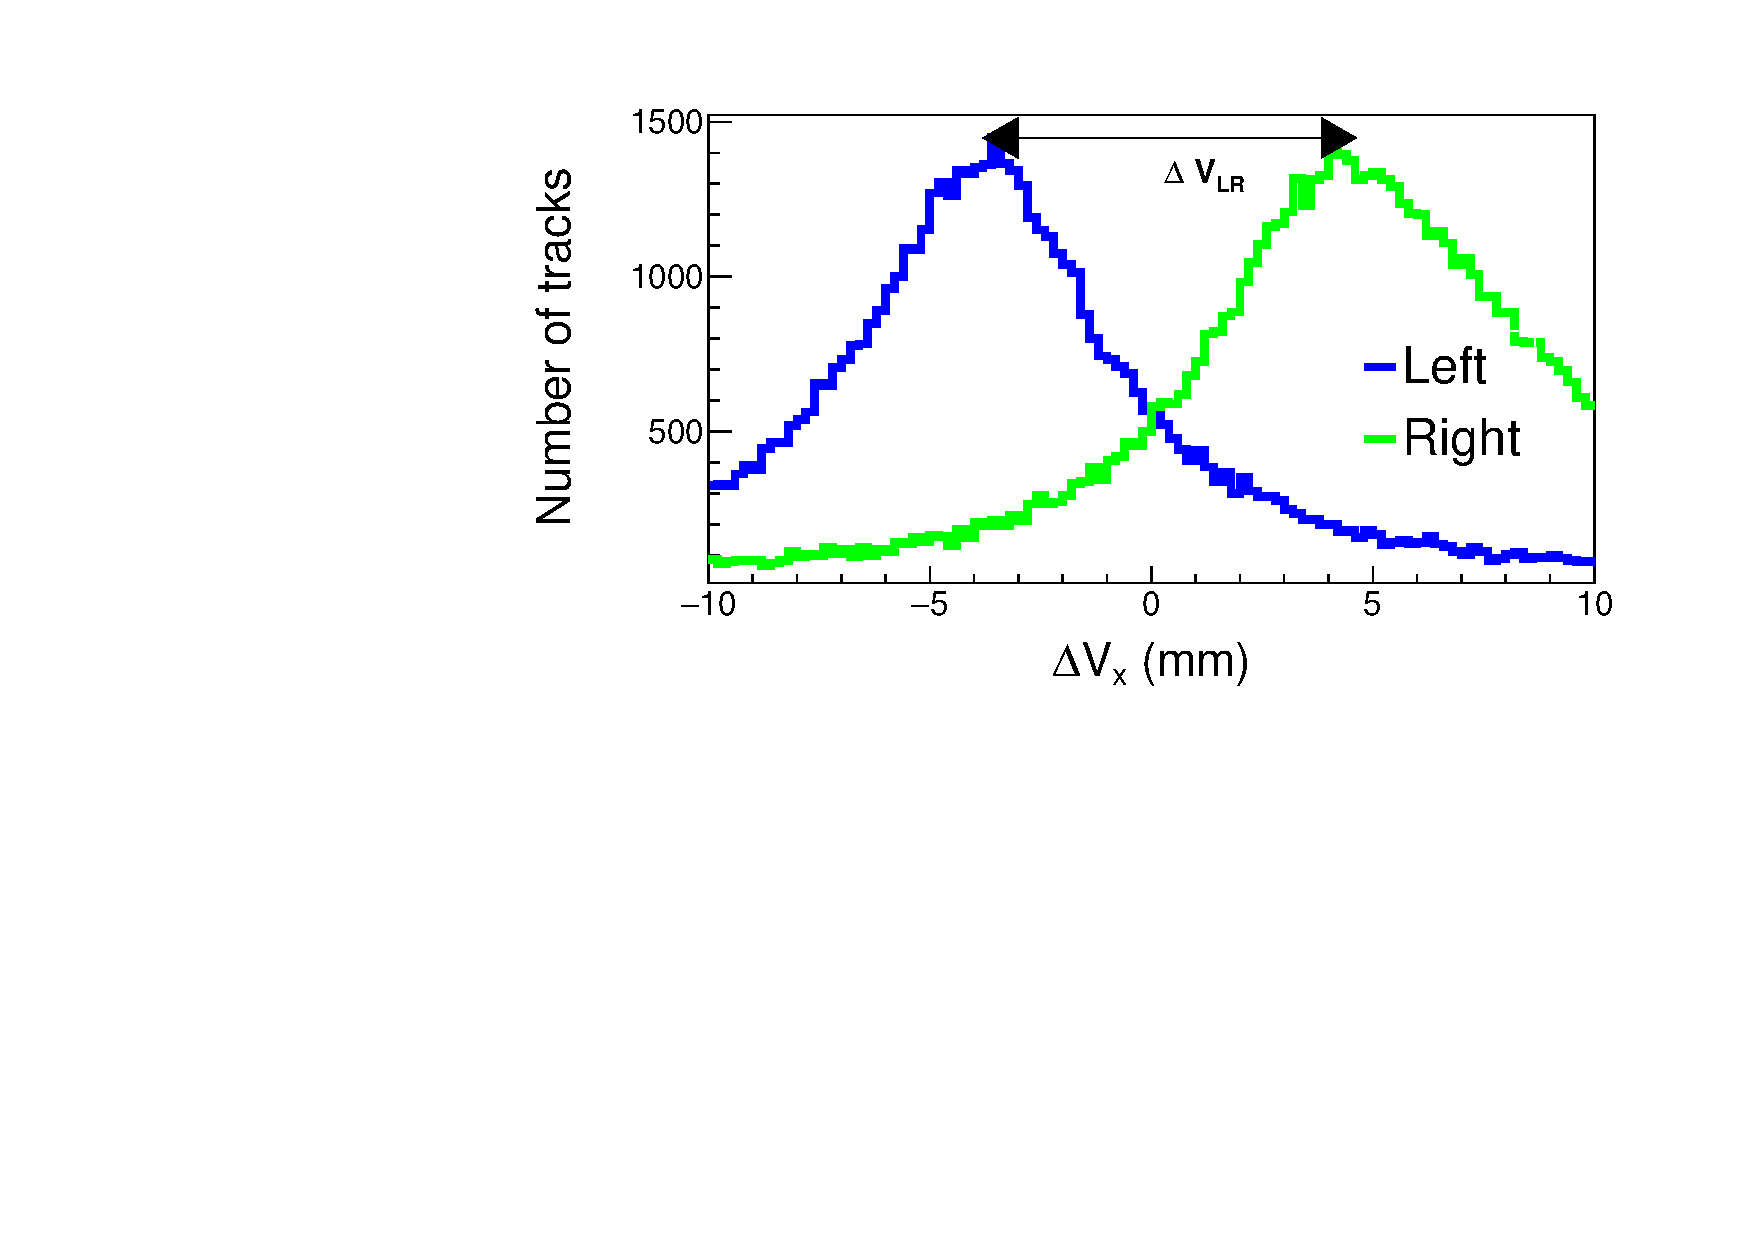
\includegraphics[width=\linewidth]{DVTP_raw.pdf}
\caption{$\Delta\mathrm{V}_\mathrm{x}$ distribution for left-going and right-going tracks in the TPC for the }
\label{fig:VLR}
\end{figure}


\begin{figure}[!htb]
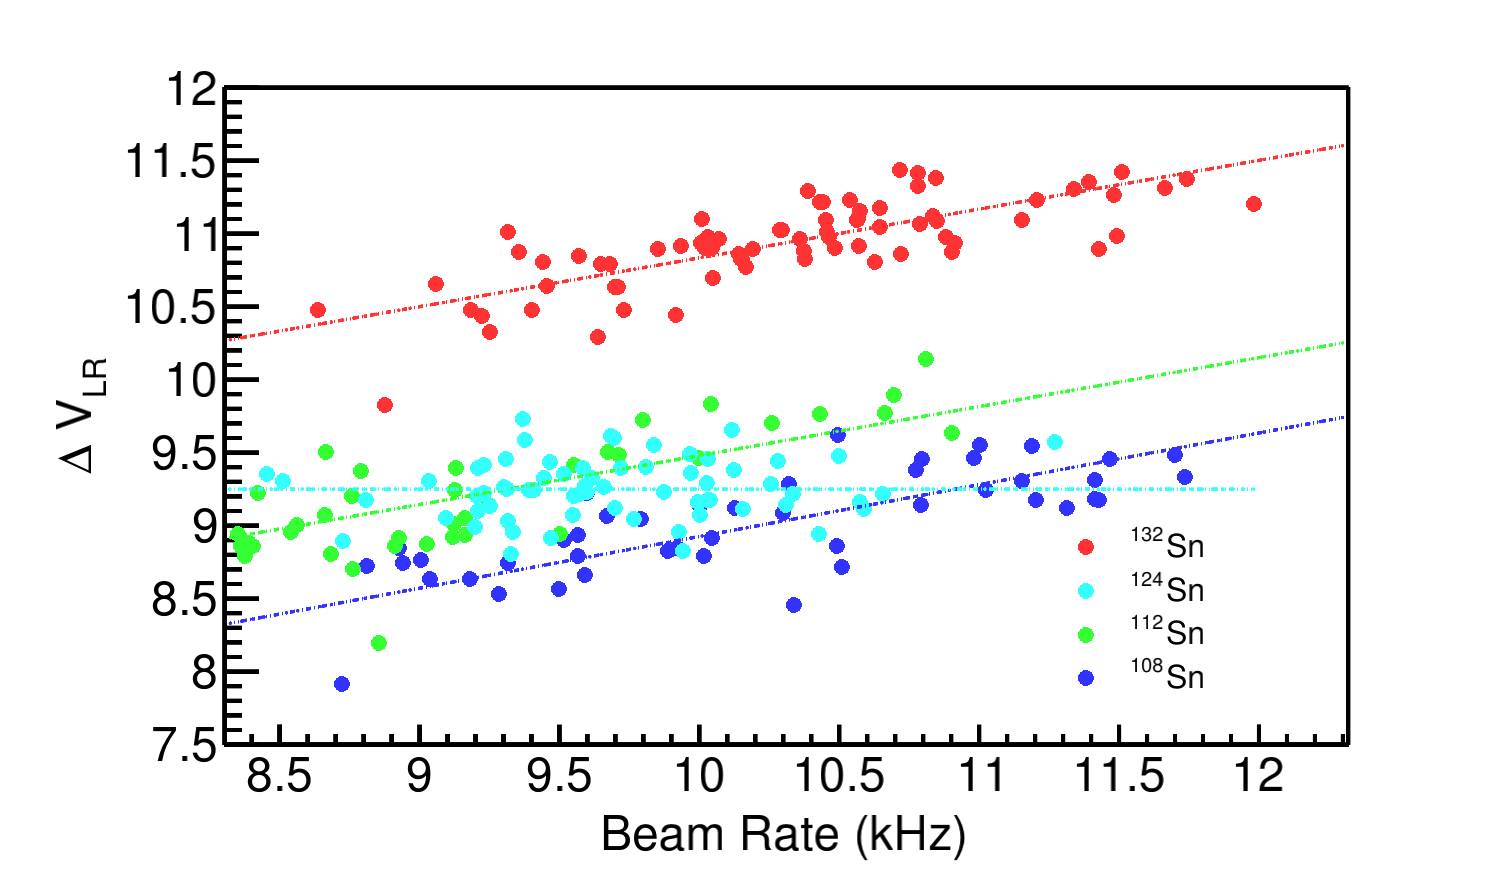
\includegraphics[width=\linewidth]{VLR_beamrate.png}
\caption{ $\Delta V_{LR}$ versus the beam rate for all systems with the fitted function.}
\label{fig:vlr_br}
\end{figure}



\begin{figure}[!htb]
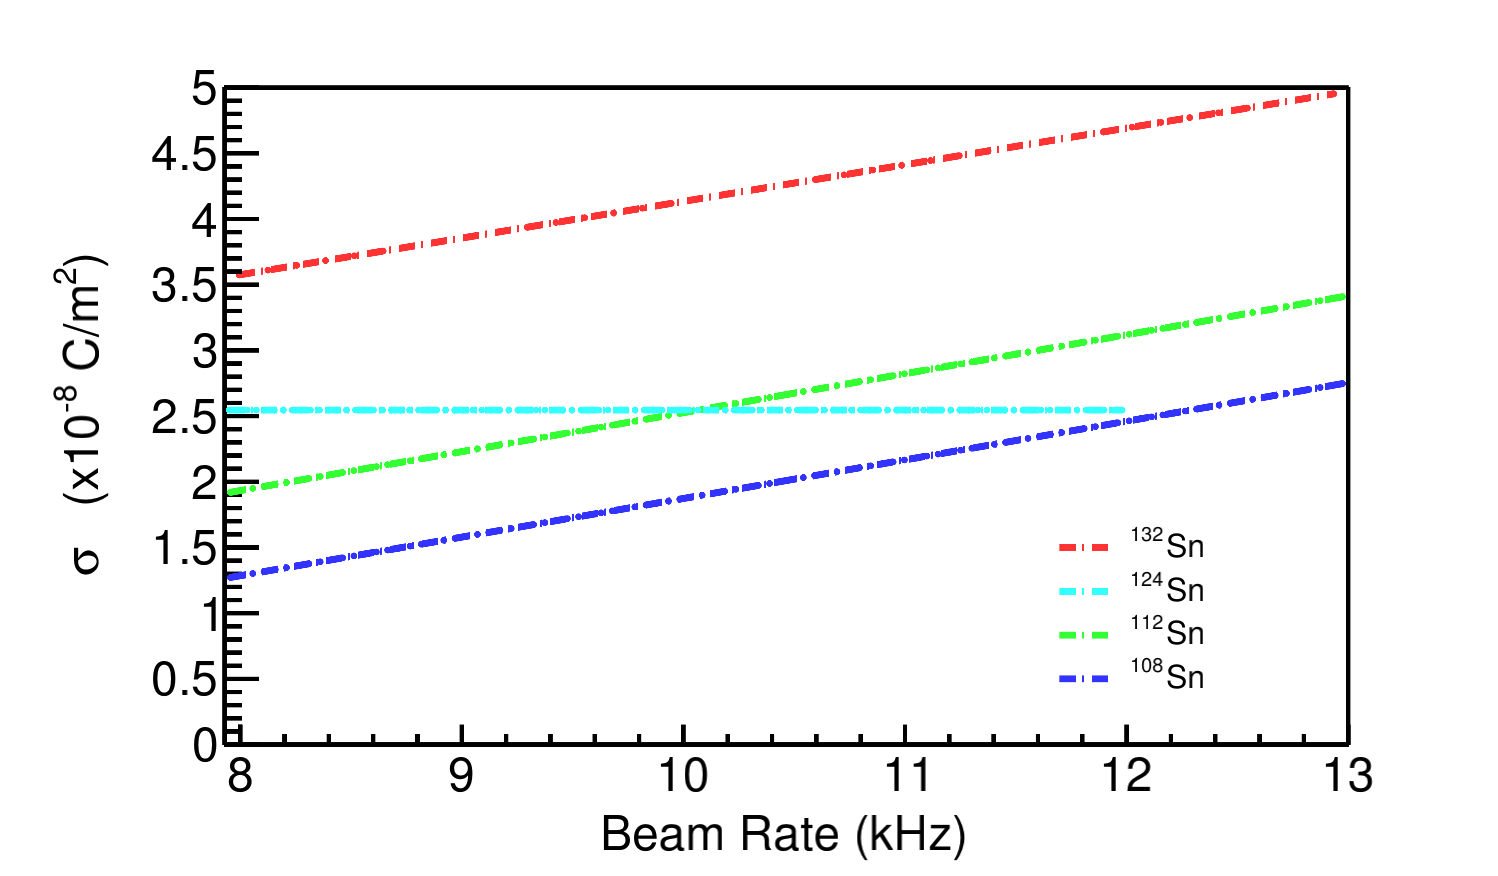
\includegraphics[width=\linewidth]{sc_beamrate.png}
\caption{Space charge fit function versus the beam rate for all systems. These are the assumed functions we use for interpolating the space charge value from the beam rate.}
\label{fig:spacechg_br_all}
\end{figure}


The average beam rate was recorded in each experimental run and slightly varied from run to run, due to beam production variations. The amount of space charge present in the field cage is directly proportional to the beam rate; therefore $\Delta\mathrm{V}_\mathrm{LR}$ is also proportional to the beam rate as shown in Fig.~\ref{fig:VLR_br}. The only parameter in the space charge correction algorithm is the surface charge density $\sigma_{\mathrm{SC}}$. Varying $\sigma_{\mathrm{SC}}$ for a wide range of values the $\Delta\mathrm{V}_\mathrm{LR}$ observable is measured and plotted in the left panel of Fig.~\ref{fig:spacechg_relation}. The surface charge density which gives $\Delta\mathrm{V}_\mathrm{LR} = 0$ is taken to be the estimate for the average amount of space charge present. 

This is done for several runs which vary in beam intensity though the solution for the estimated space charge value will be different. Since the surface charge density is proportional to the beam rate, a linear fit gives good agreement for interpolating the surface charge values as a function of beam rate. Figure~\ref{fig:spacechg_relation} shows the relation of the dependence of the space charge as a function of beam rate for the ${}^{132}$Sn system.

\begin{figure}[!htb]
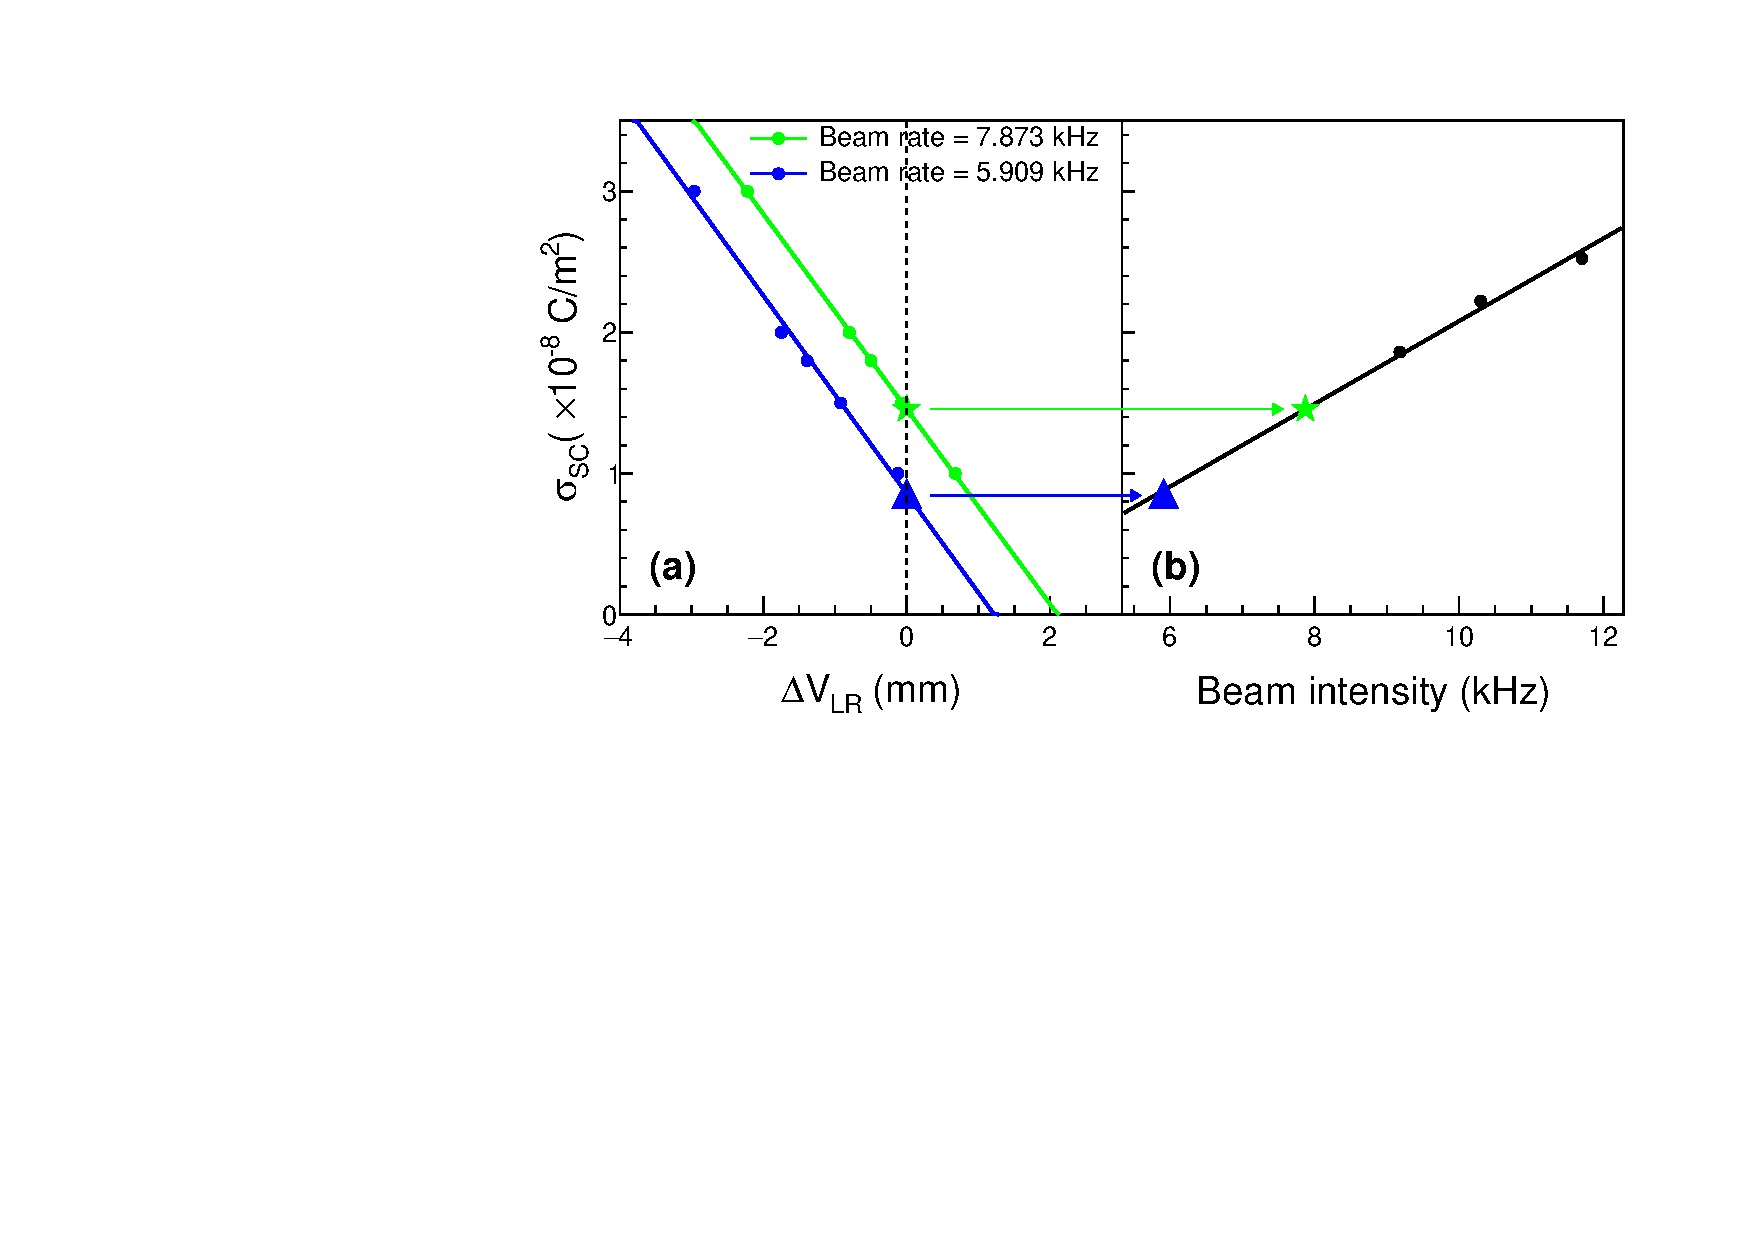
\includegraphics[width=\linewidth]{SC_Relation.pdf}
\caption{Space charge relation}
\label{fig:spacechg_relation}
\end{figure}


Following this algorithm the space charge is estimate for each run and system. Figure~\ref{fig:scDensity} shows the summary of the extracted space charge values for each secondary beam. The linear fits relating the space charge density to the beam rate for each system is shown in Fig.~\ref{fig:spacechg_br_all} where the space charge value is inferred from the measured beam rate. Notice that in the $\tin{112}{124}$ system a constant value of was assumed since the beam rate did not span a large enough range to warrant a more detailed analysis. 

%What is the best figure to put in? VLR vs Charge density? 
%estimate of the error of VLR and how it corresponds to charge density

\begin{figure}[!htb]
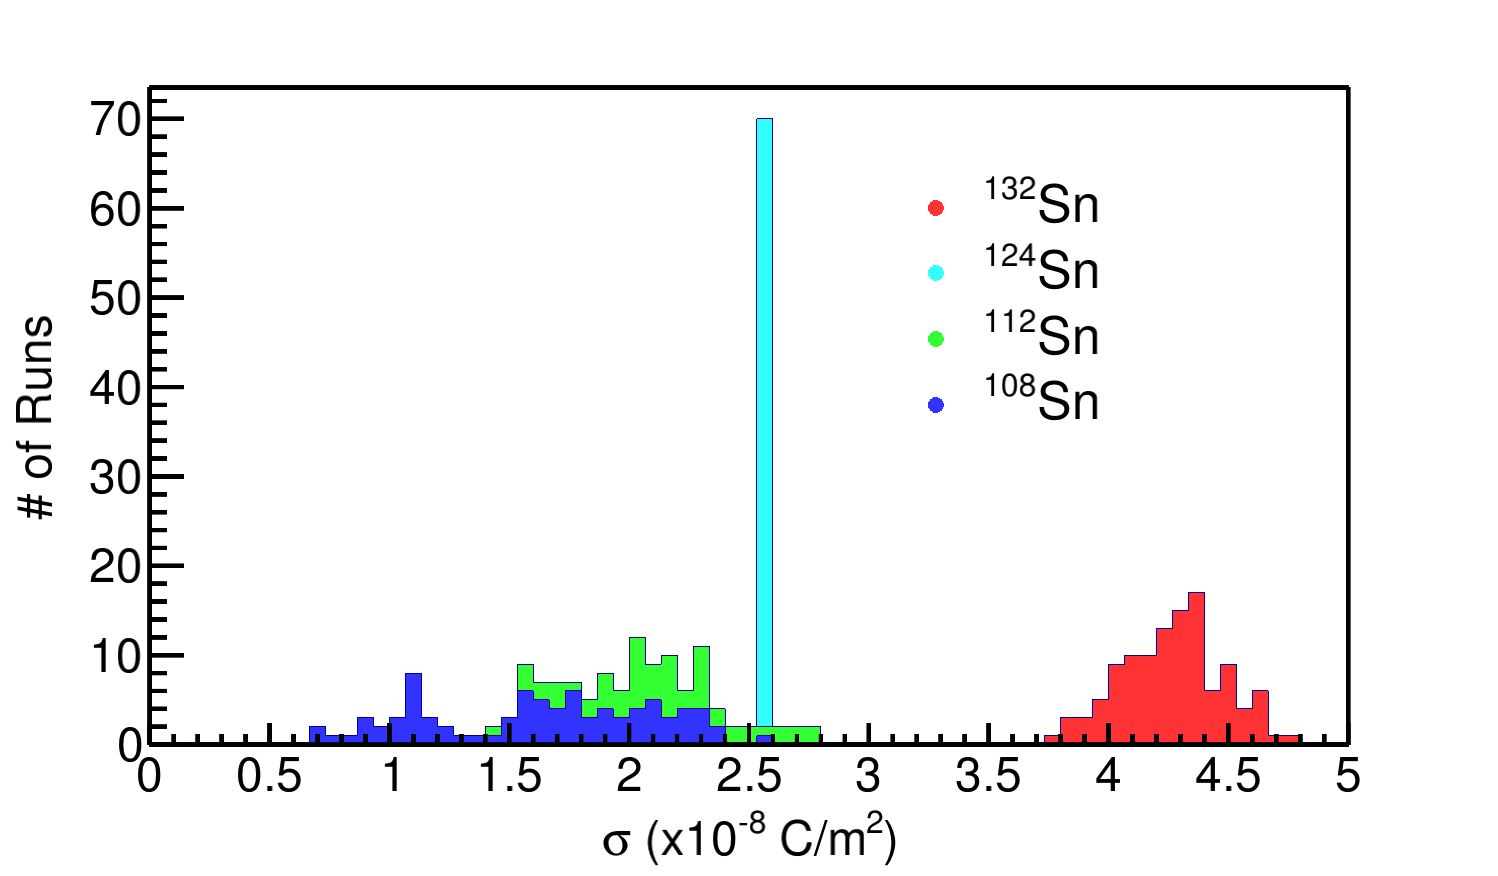
\includegraphics[width=\linewidth]{spaceChgDensity.png}
\caption{Distribution of estimated space charge densities for each beam type.}
\label{fig:scDensity}
\end{figure}



\begin{figure}[!htb]
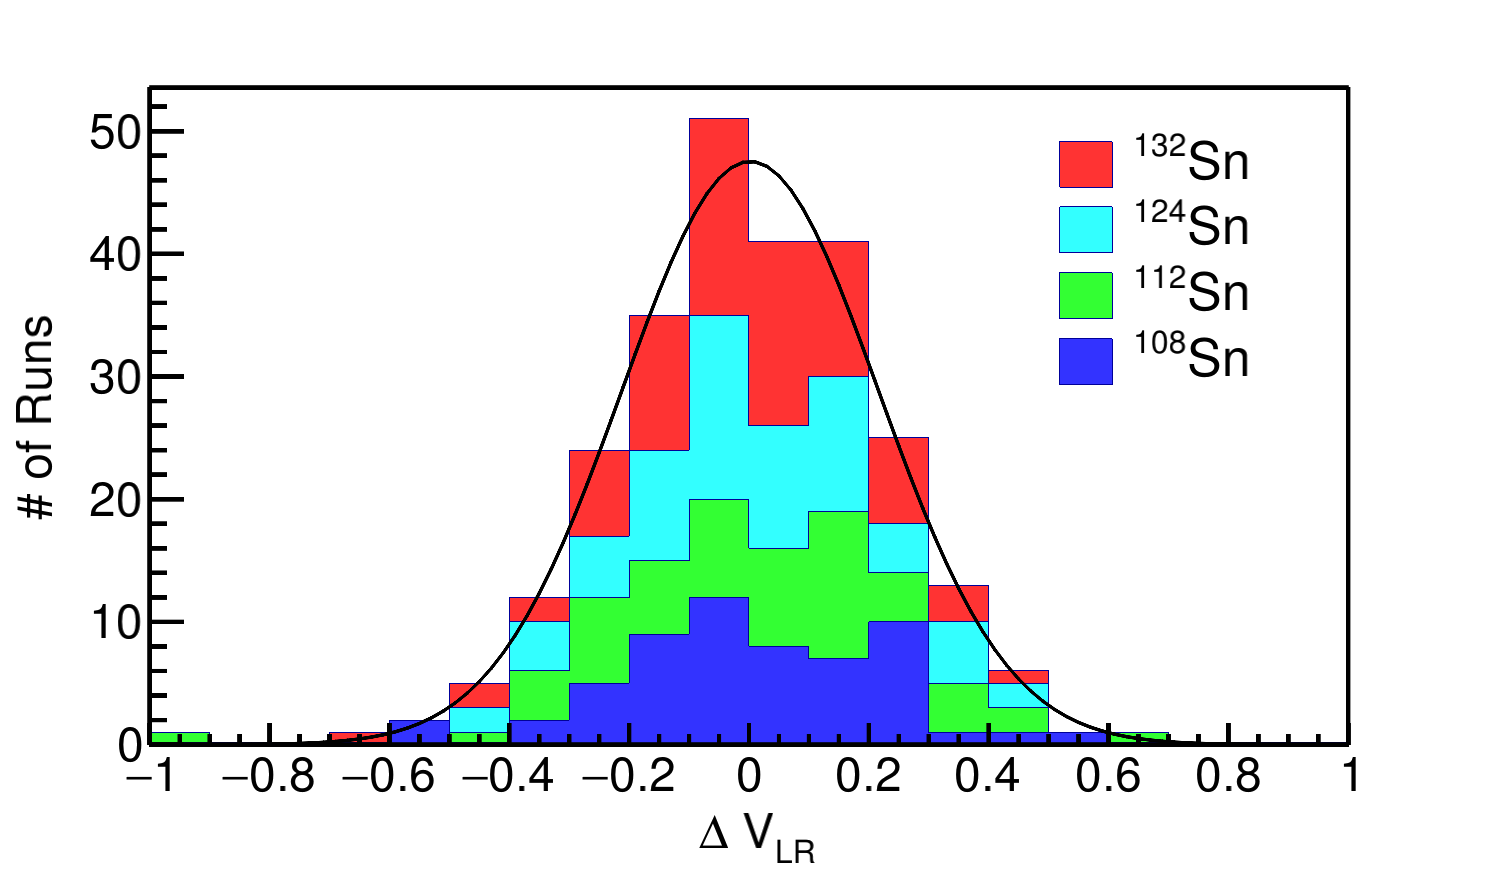
\includegraphics[width=\linewidth]{VLRresidual.png}
\caption{Residuals in the fitted line of $\Delta V_{LR}$ observable for all systems.}
\label{fig:vlrResidual}
\end{figure}

Adding the BDC vertex greatly improves the momentum resolution of the track fitting, but there is a systematic shift when as compared with the momentum value without using a vertex as an extra constraint. Since the space charge affects right-going and left-going tracks differently making right-going tracks differently than left-going tracks, it appears they no longer originate from the BDC which is not affected by the space charge. For tracks at polar angles of $\theta < 40 \deg$, the disagreement between momentum values with and without the BDC are much less because the projection of the track does not disagree as much with the BDC point as shown in Fig.~\ref{fig:mom_S_before}. Figure~\ref{fig:mom_L_before} shows the momentum value of tracks going at polar angles of $\theta > 40 \deg$ are more sensitive to small changes in the BDC when including it as an extra constraining point. After correcting for the space charge, adding the BDC point as an extra constraint on the track does not bias the reconstructed momentum value for either $\theta < 40 \deg$ or $\theta > 40 \deg$, which has the greatest improvement, as seen in Fig.~\ref{fig:mom_S_after} and Fig.~\ref{fig:mom_L_after} respectively. Recall that only the relative distance between left and right-going tracks was minimized; there was no guarantee that the corrected tracks coincide with the absolute BDC position at the target. This is one of the evidences of the correction's success. The others being the agreement with the expected cocktail calibration beam as described above. Later we will show how the space charge corrects the momentum distributions of left and right-going pions in the TPC. 


\begin{figure}[!htb]
    \centering
    \begin{subfigure}[t]{0.45\textwidth}
        \centering
        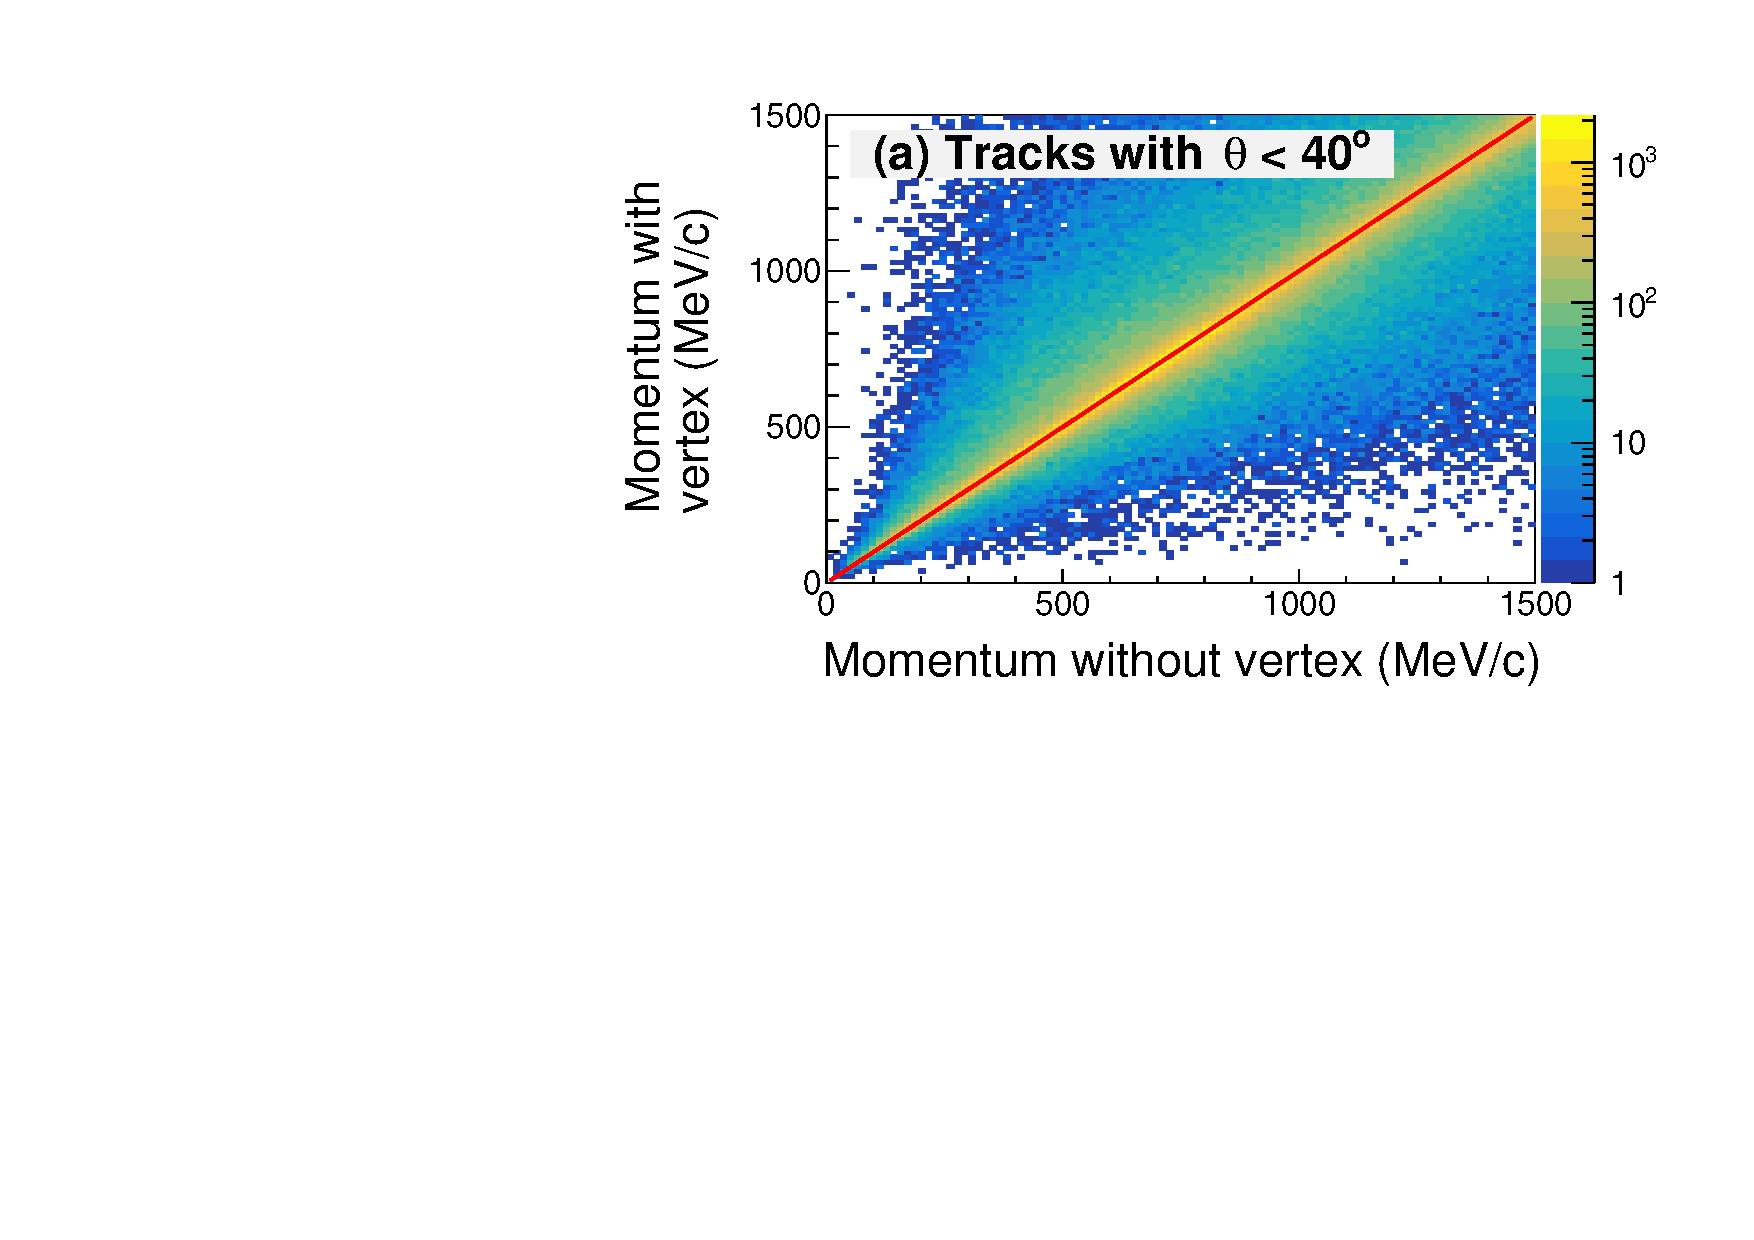
\includegraphics[width=\linewidth]{BDC_P_small_angle.pdf} 
        \caption{Generic} \label{fig:mom_S_before}
    \end{subfigure}
    \hfill
    \begin{subfigure}[t]{0.45\textwidth}
        \centering
        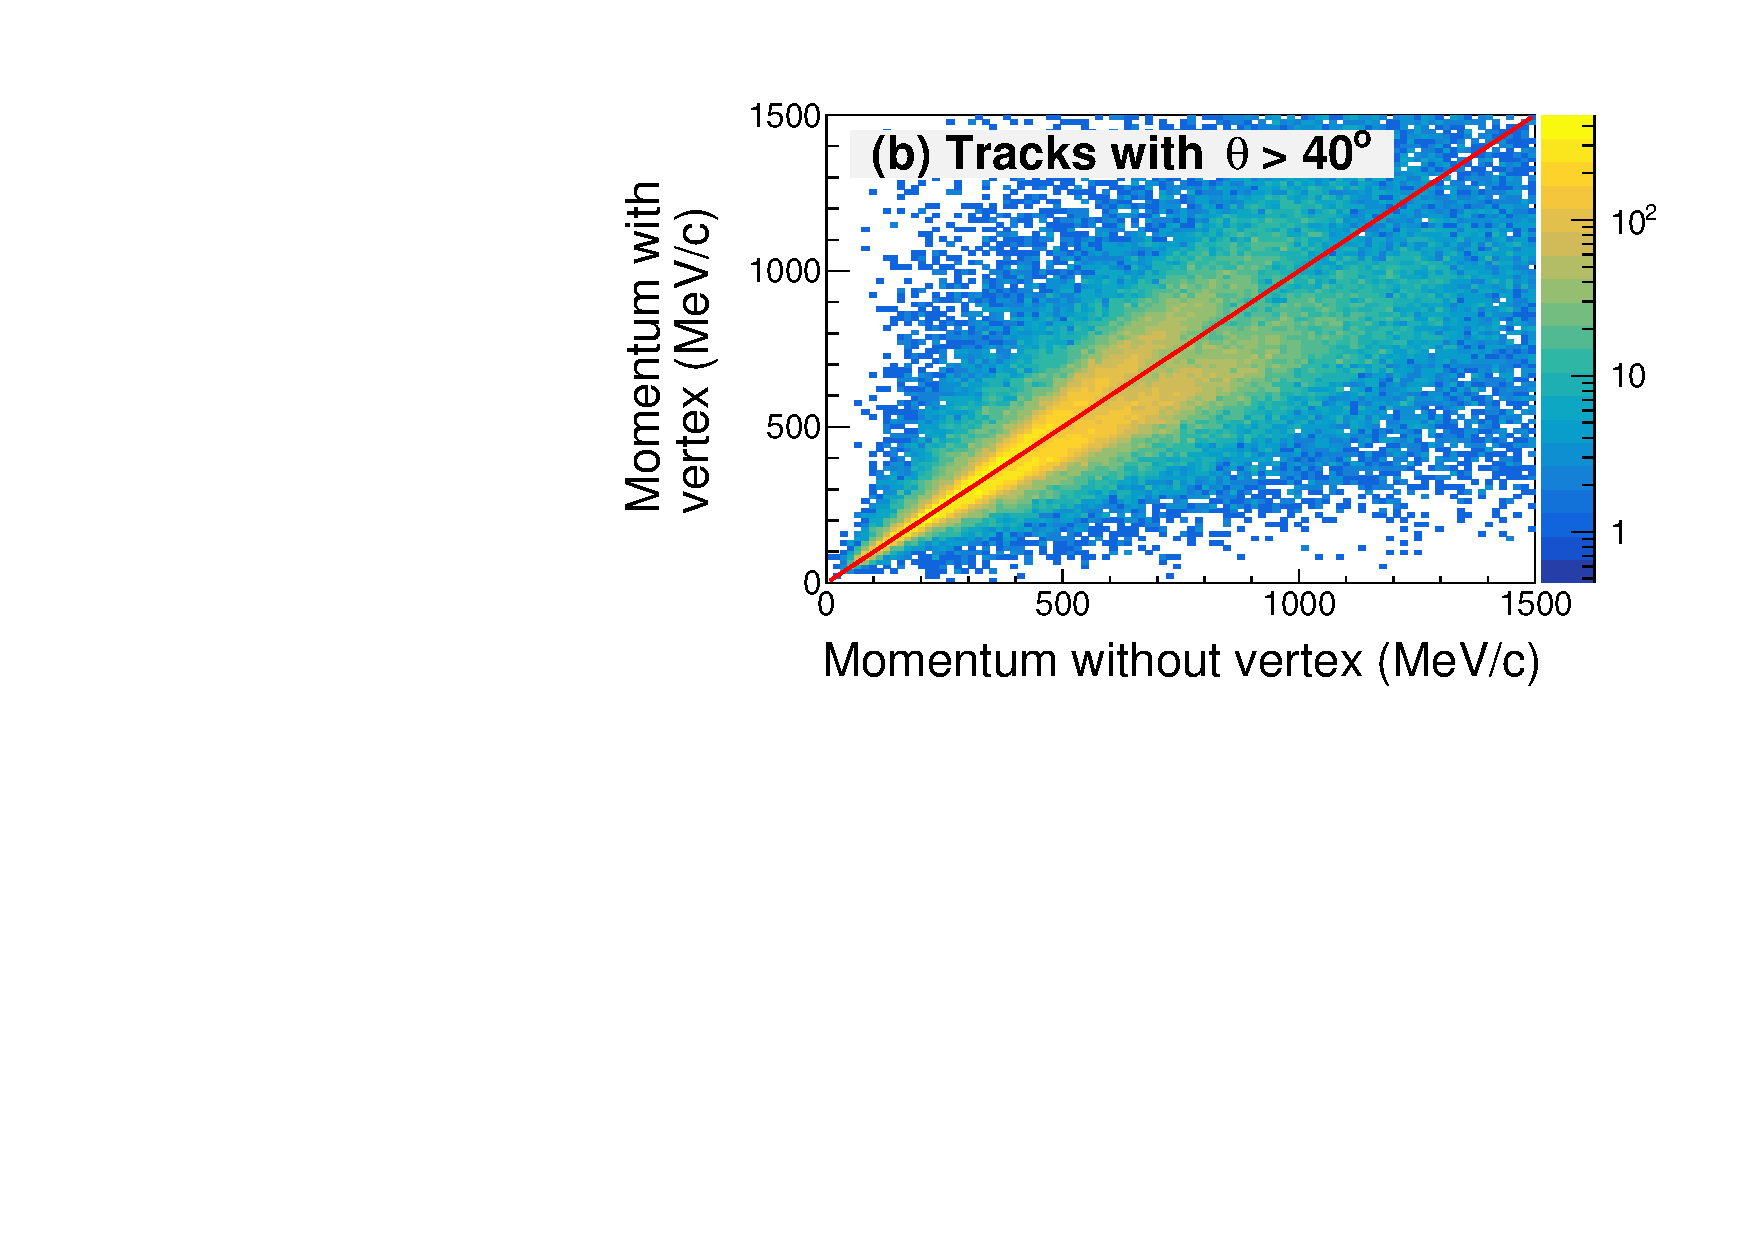
\includegraphics[width=\linewidth]{BDC_P_large_angle.pdf} 
        \caption{Competitors} \label{fig:mom_L_before}
    \end{subfigure}
    
    \begin{subfigure}[t]{0.45\textwidth}
        \centering
        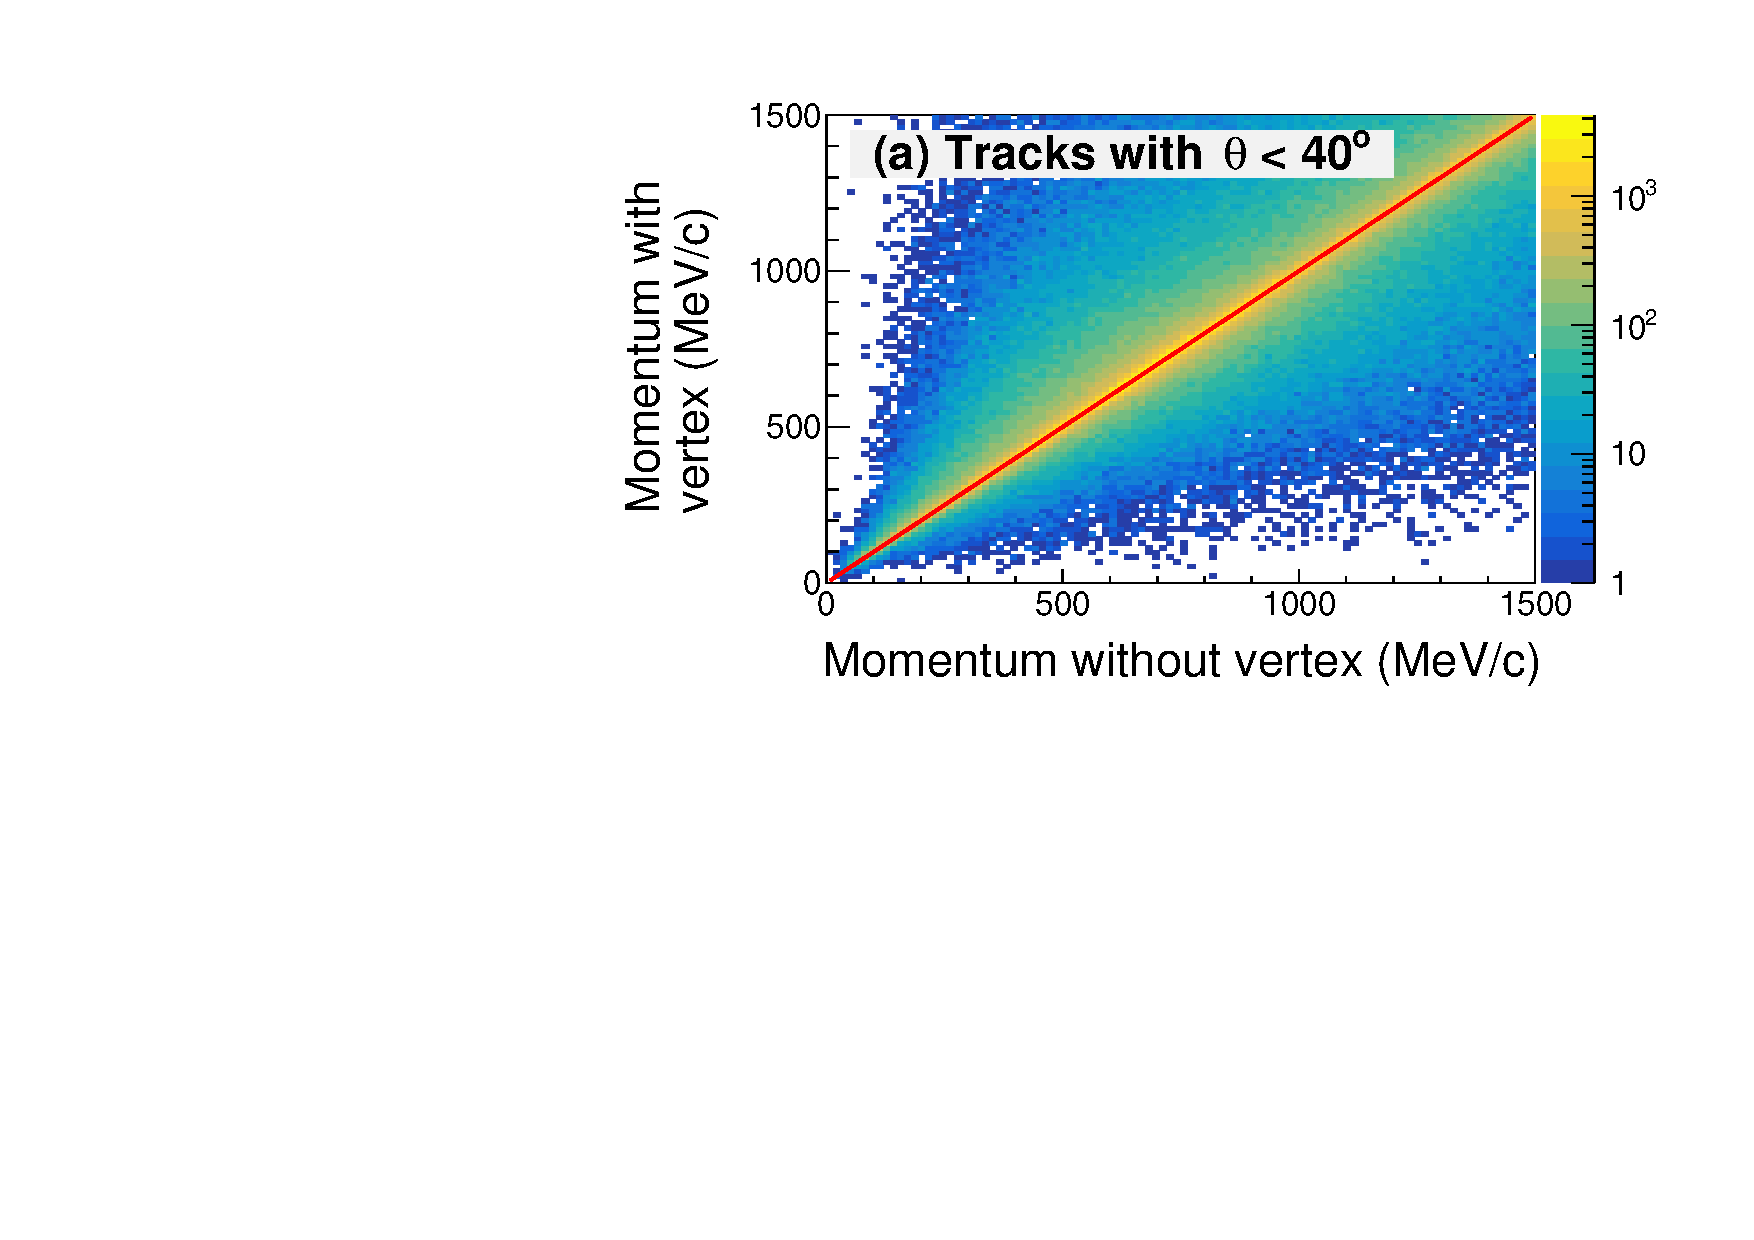
\includegraphics[width=\linewidth]{BDC_P_aftercor_small_angle.pdf} 
        \caption{Generic} \label{fig:mom_S_after}
    \end{subfigure}
    \hfill
    \begin{subfigure}[t]{0.45\textwidth}
        \centering
        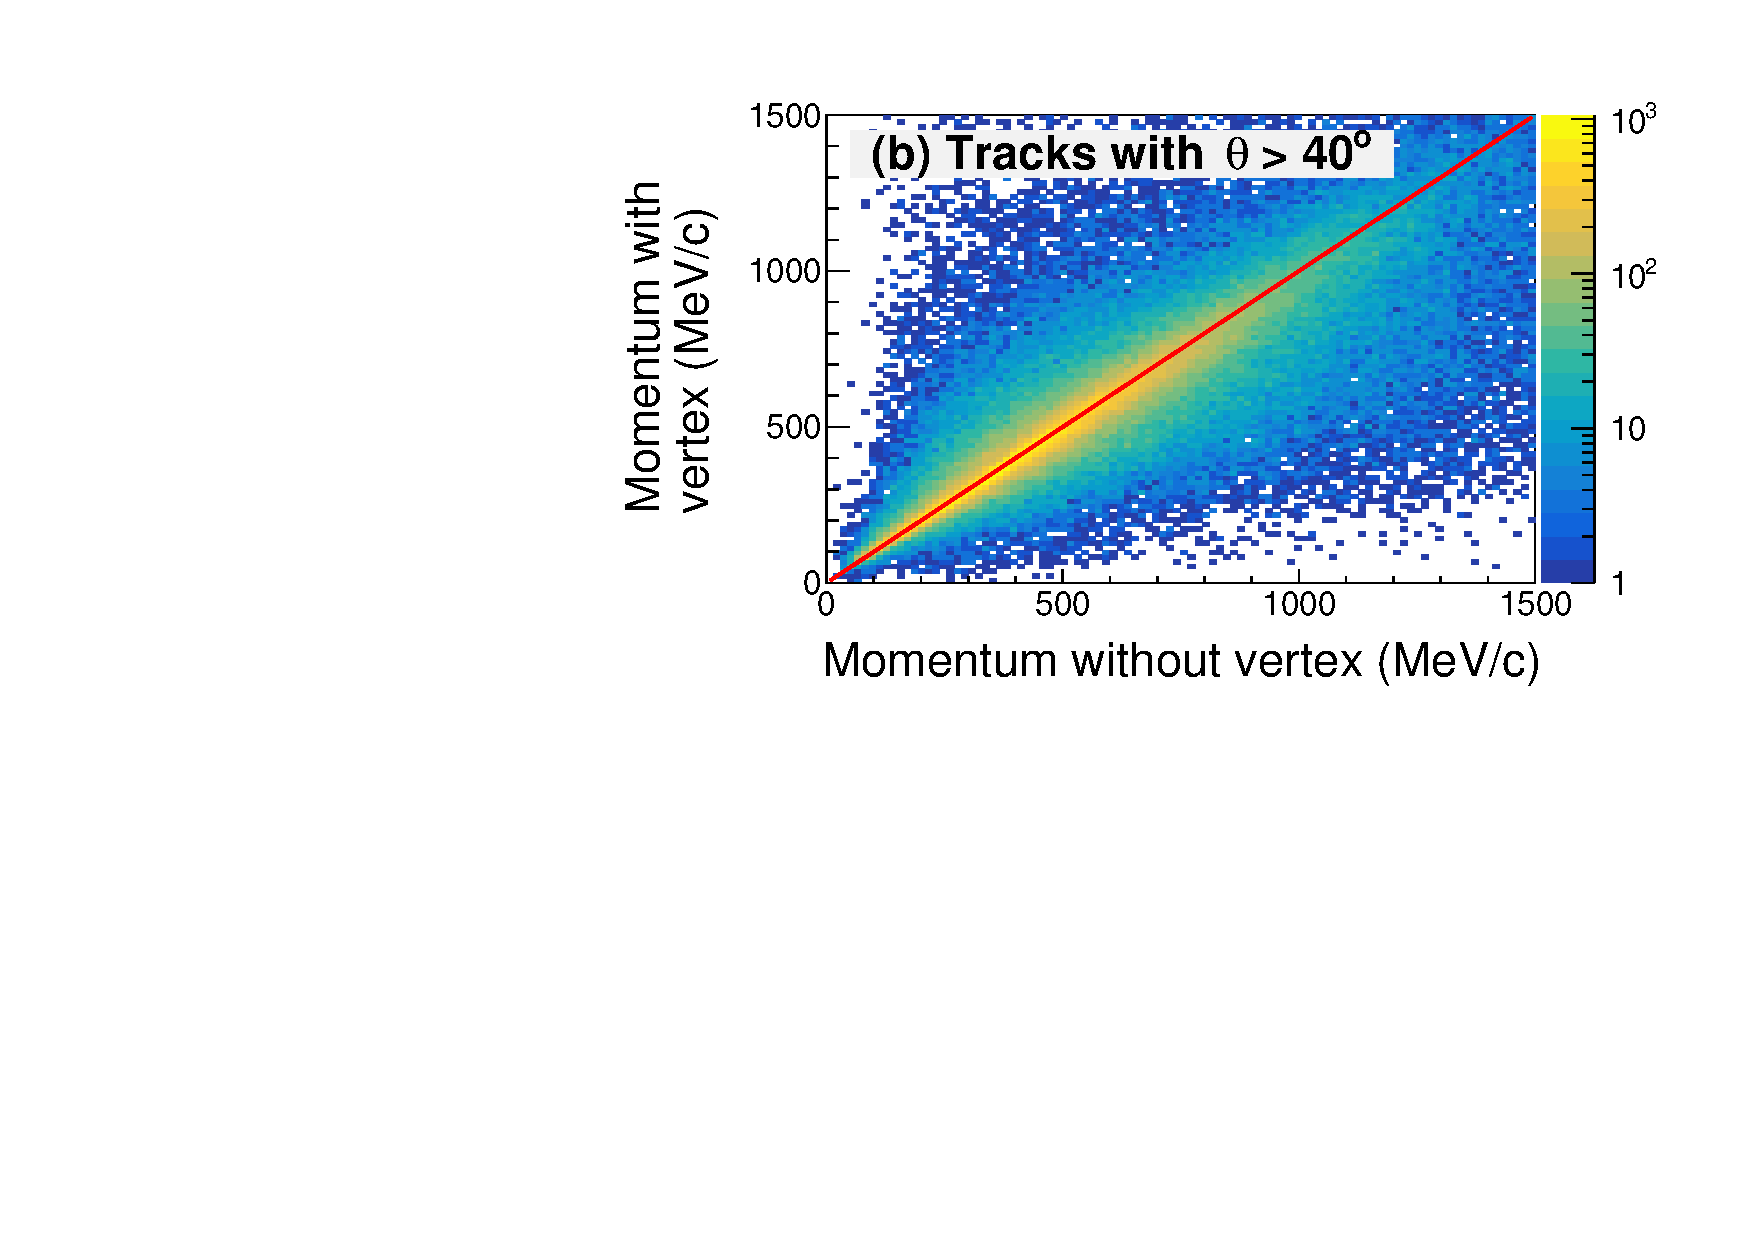
\includegraphics[width=\linewidth]{BDC_P_aftercor_large_angle.pdf} 
        \caption{Competitors} \label{fig:mom_L_after}
    \end{subfigure}
\label{fig:mom_sc}
\end{figure}


\begin{comment}

\begin{figure}[!htb]
    \centering
    \begin{subfigure}[t]{0.49\textwidth}
        \centering
        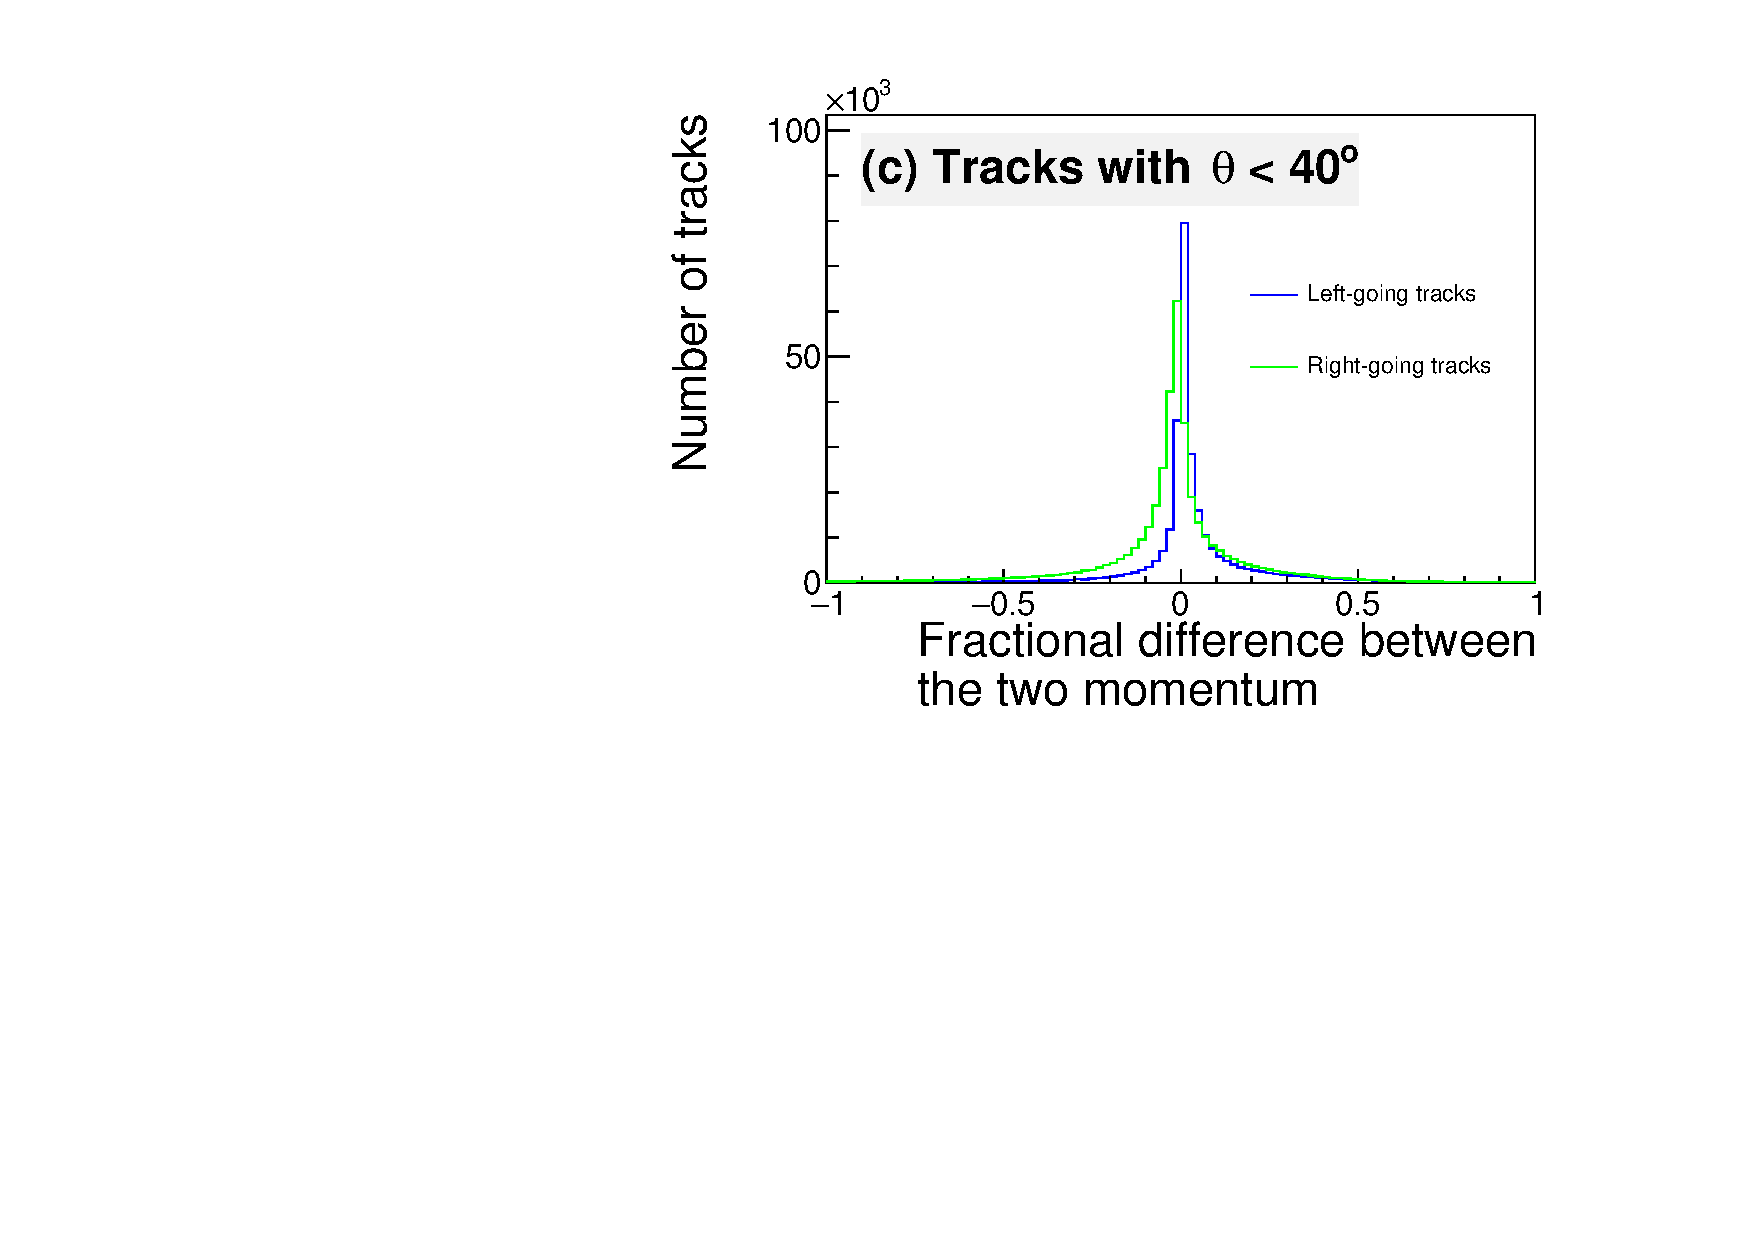
\includegraphics[width=\linewidth]{BDC_P_frac_small_angle.pdf} 
        \caption{Generic} \label{fig:mom_S_1D}
    \end{subfigure}
    \hfill
    \begin{subfigure}[t]{0.49\textwidth}
        \centering
        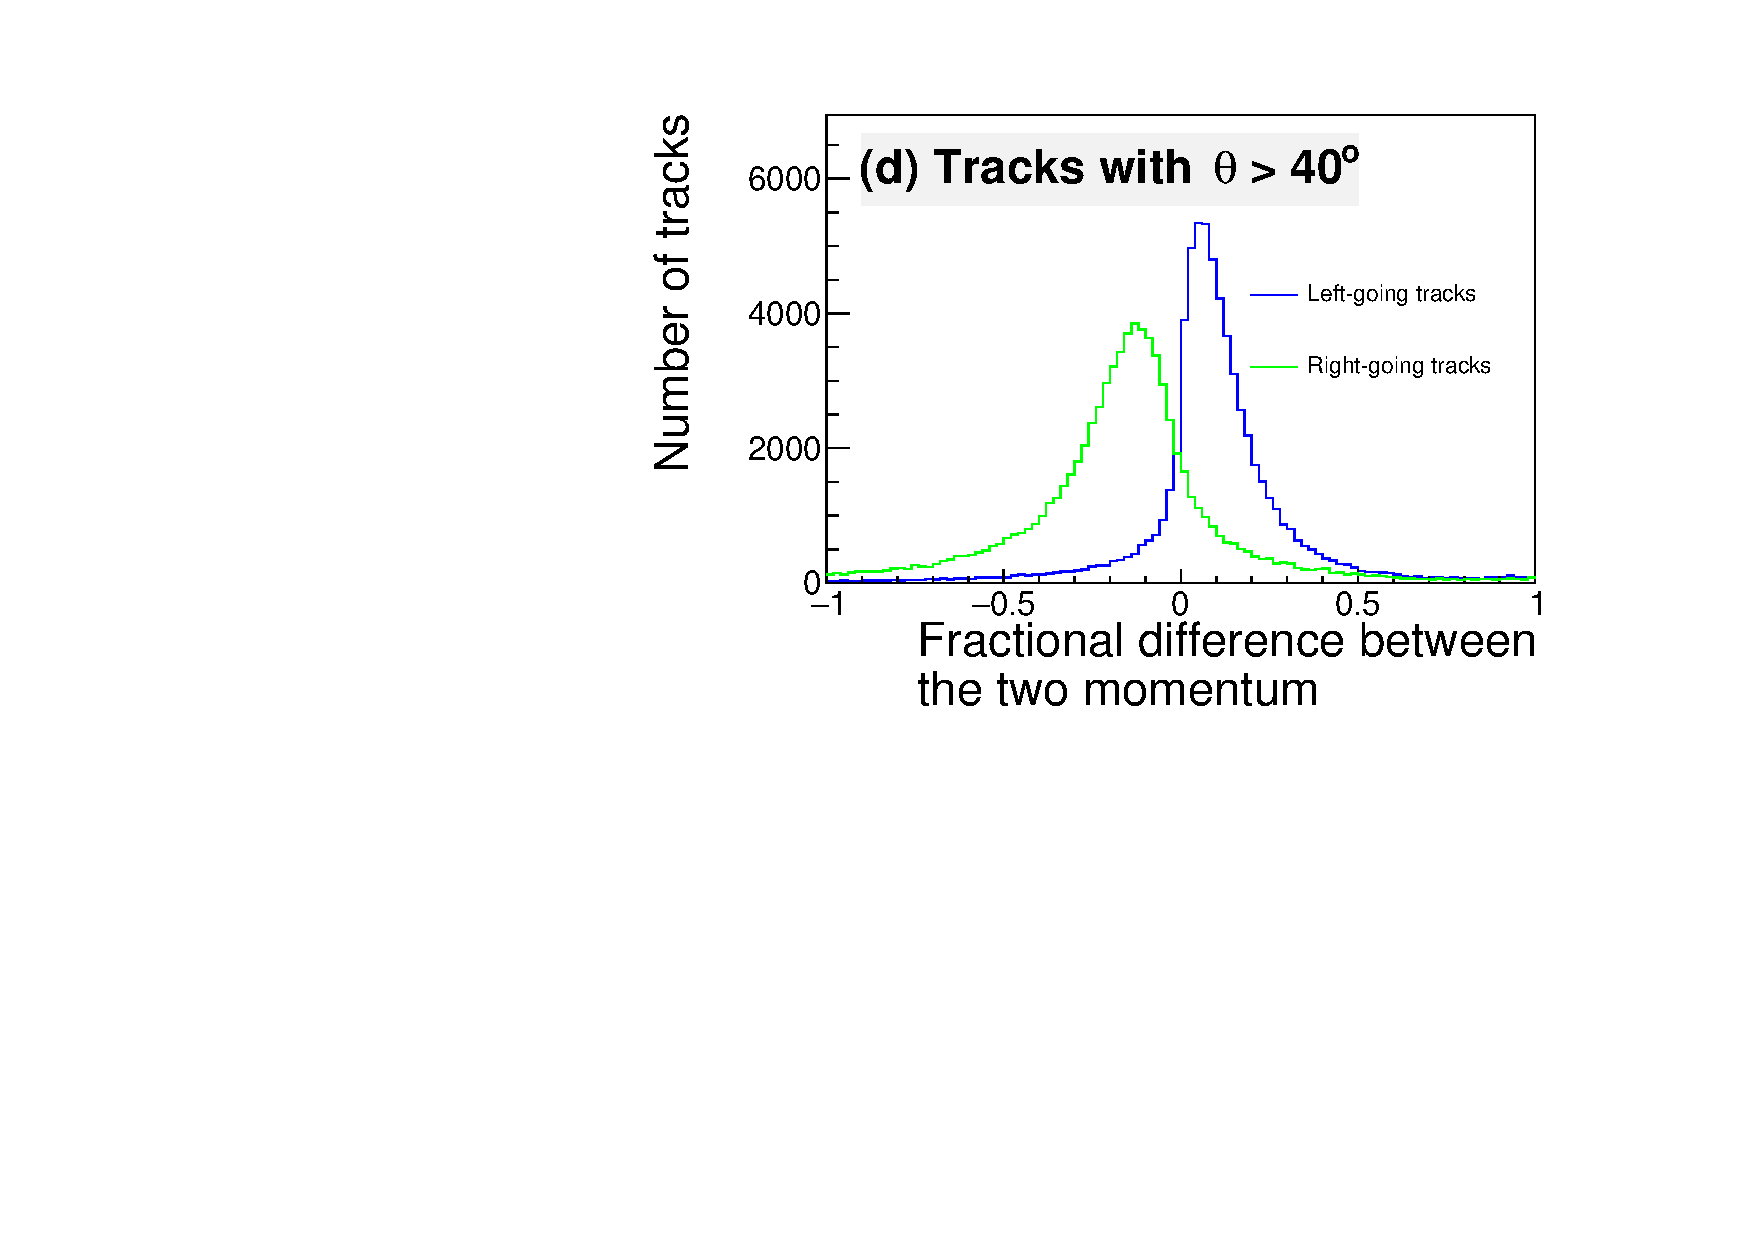
\includegraphics[width=\linewidth]{BDC_P_frac_large_angle.pdf} 
        \caption{Competitors} \label{fig:mom_L_1D}
    \end{subfigure}
    
\label{fig:mom_1D}
\end{figure}
\end{comment}


%Reference appendix for poisson solver 
%Tables for ion drift velocity in P-10 Gas reference Sauli
%Figure of sDAC or POCA 
%Figure of cartoon of what is happening to tracks
%Figure of correction map in TPC and MC map 
%Figure of before and after correction BDC vs reco momentum
%Figure of track residuals before and after?



\section{Monte Carlo Simulation}
The monte carlo (MC) simulation is composed of two separate simulations. The first simulation is an accurate model of the fundamental interactions of a particle passing through the various materials in the TPC; to accomplish this we have modled everything in Geant4 which also provies a particle generator. A scale model of field cage, front window, front window frame, pad plane, and aluminum top plate are modeled with the correct material type and dimensions assuming P-10 gas at a density of 1 atm. The magnetic field map of the SAMURAI dipole magnet was imported into Geant4 as well after assuming rotational symmetry along the axis perpendicular to the pole face. Along with the energy loss and particle transport, Geant4 also handles multiple scattering, and particle decay. The output of the particle generator is a series of energy loss points which contain the amount of energy lost in $\si{\kilo\electronvolt\per\centi\metre}$ and the location of the energy loss in Cartesian space $(x,y,z)$. 

In the second part of the MC simulation, the physical processes involved in the operation and measurement of the TPC are simulated, such as the electron drift, avalanche process, and all processes involved in the signal creation in the electronics, simulating the detector's response to a MC track. This is separated into three software tasks, the drift, pad response, and electronics tasks. In the following section we will discuss these tasks in more detail, the discussion of Geant4 is not covered here and is left to the reader to explore.  

\subsection{Drift Task}
 The first step of the drift task is to convert the primary ionization points of the MC track provided by Geant4 into electrons. The average number of electrons created in a gas,$N_{e^-}$, can be described as,
\begin{equation}
N_{e^{-}} =  \frac{\Delta E}{I},
\label{eq:kev2el}
\end{equation}
 
where $I$ is the ionization coefficient of P10 gas (Table~\ref{tb:gas}) and $\Delta E$ is the energy loss deposited in units of \si{\electronvolt}. Since the electric field set up by the field cage is uniform for the most of the area covered by the pad plane, we assume a straight line trajectory for each electron until it reaches an anode wire. The total length drifted from the initial primary ionization point to the final anode wire is given by $L_{anode}$. 

\begin{table*}\centering
\ra{1.3}
\begin{tabular}{@{}rr@{}}\toprule 
\multicolumn{2}{c}{Electron Transport Gas Properties} \\
 \midrule
Drift velocity & 5.53 $\si{\centi\meter\per\micro\second}$\\
Transverse diffusion & 240 $\si{\micro \meter \centi\meter}^{-1/2}$\\
Longitudinal diffusion &  340 $\si{\micro \meter \centi\meter}^{-1/2}$\\
Gas Ionization & 26.2 $\si{\eV}$\\
\bottomrule
\end{tabular}
\caption{An overview of the properties of the TPC}
\label{tb:gas}
\end{table*}

Drifting electrons frequently collide with the detector gas causing them to change direction. This stochastic motion is  described by a a diffusion process occurring along the direction of travel (longitudinal) and transverse to the motion. The longitudinal ($c_{l}$) and transverse ($c_{t}$) diffusion coefficients are determined by Garfield++ calculation in the presence of a \SI{0.5}{\tesla} magnetic field, listed in Tb.~\ref{tb:gas}. The diffusion process is modeled by randomly sampling from a Gaussian distributions describing both of the directions. The random shift is then added to the final position of the electron. The deviation in the transverse direction, $dr$, is randomly sampled from,

\begin{equation}
dr = e^{-\frac{r^2}{2\sigma_{t}^2}},
\end{equation}

where $\sigma_{t}=c_{t}\cdot\sqrt{L_{anode}}$.The Cartesian directions are given by $dx = dr \cdot \cos(\alpha)$ and $dz = dr \cdot \sin(\alpha)$, where $\alpha$ is a random angle from 0 to 2$\pi$, since there is no preferential angle  of emission in the transverse plane. The shift associated with the longitudinal diffusion, $dl$, is randomly sampled from, 

\begin{equation}
dl = e^{-\frac{t^2}{2\sigma_{l}^2}},
\end{equation}

where $\sigma_{l}=c_{l}\cdot\sqrt{L_{anode}}$. 

The final position of the electron along the wire is calculated  $x' = x + dx$. Since the electron will terminate on the closest anode wire the anode wire that is closest to the shifted z-position $z\textprime = z + dz$, the final electron z position is then updated to the anode wire it terminated on. The total drift time of the electron $t$ is calculated as,

\begin{equation}
 t = \frac{L_{anode} + dl}{v_d} + t_{offset},
 \label{eq:electronTime}
\end{equation}
 
 where $v_d$ is the drift velocity. The parameter $t_{offset}$ aligns the MC time bucket spectrum with the data. This is because the y-position corresponding to time zero in the data time bucket spectra does not correspond to the same position in the MC for time zero.  This value was found to be \SI{23}{\nano\second} by aligning the MC vertex to the data vertex.

The total number of electrons produced in the avalanche process of a single electron was simulated in Garfield++ as seen in Fig.~\ref{fig:gaincalib} for the anode wire voltages used in the experiment. The number of electrons produced in the avalanche is randomly sampled from the corresponding distribution depending on which anode wire section the electron terminated; the number of electrons produced is stored as a number instead of multiple instances of the original electron to save space and computation time. We assume that the lateral movement along the wire arising form $\vec{E}\times\vec{B}$ effect near the wire is negligible as compared with diffusion and other effects described later. 

It is worth mentioning there is the possibility to simulate the space charge effects in this class where the inverse to the correction map described in \ref{sec:spacecharge} is applied to the drifting electrons. This is not used for calculating the response of the TPC for efficiency calculations since it is a trivial exercise to input the space charge map and correct for it using the same inverse map.  

\subsection{Pad Response Task}
The total charge of each avalanche must be distributed according to the pad response function (PRF) described in section \ref{sec:prf}. The PRF is simulated as the double integral of a 2-dimensional Gaussian. The final output charge on all the pads are the superposition of the PRFs of all drifted electrons. The MC PRF is expressed as, 

\begin{equation}
PRF(x,z) = \iint e^{-\frac{(x-x_o)^2}{2\sigma_x^2}} e^{-\frac{(z-z_o)^2}{2\sigma_z^2}}dxdz,
\end{equation}

where $\sigma_x = 3.4$ and $\sigma_z = 3.5$, and $x_0$ and $z_0$ are the final position of the drifted electron. The $\sigma$ parameters were determined through an iterative comparison matching the PRFs of the MC and experimental data sets. 


\subsection{Electronics Task}

The purpose of the electronics task is to simulates the electronics response to the charge induced on each pad, converting charge into ADC channels. The induced current in the pad goes through a pre-amplifier and shaping amplifier which determine the final pulse shape that is read out. The pulse shape did not change significantly in any circumstance, such as pulse height, data type, or particle type, as long as the electronics settings are fixed. This allows us to assume the pulse shape is constant and can be described by two variables, the height of the pulse, $Q$, and the starting time bucket of the pulse, $t_o$. The starting time of the pulse is defined as the time at 10\% of the rising edge. The shape of the pulse depends on the shaping time constant which was set to \SI{117}{\nano\second} for the data analyzed here. Figure~\ref{fig:pulseshape} shows the pulse shape which was extracted from the experimental signals in the data. These were signals that did not saturate the electronics and was averaged over a wide range of ADC values. Here it is normalized so the maximum height is 1. 



\begin{figure}[!htb]
    \centering       
    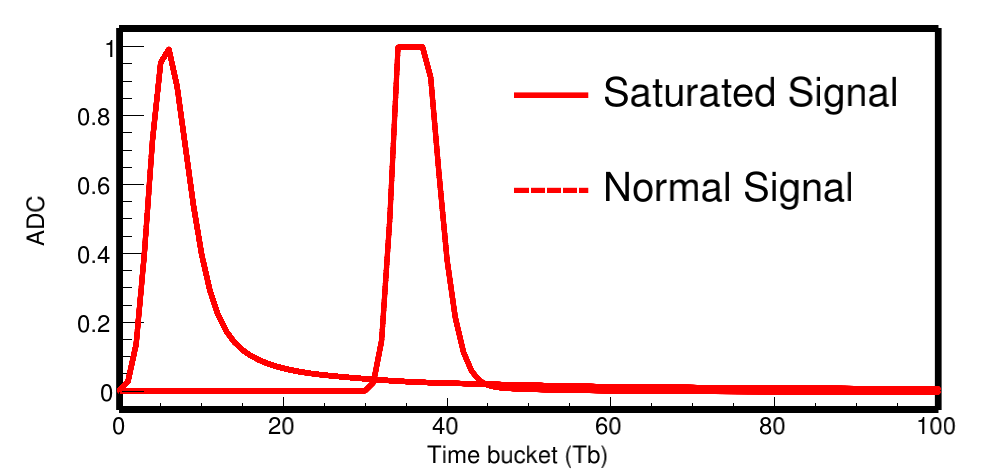
\includegraphics[width=\linewidth]{satpulse.png} 
    \caption{Standard pulse }
    \label{fig:pulseshape}
\end{figure}


Converting the charge in each pad into the height of the ADC response in the electronics is calculated as, 

\begin{equation}
Q = f_G  A_{tot} \cdot e \cdot\frac{ADC_{max} - ADC_{pedestal}}{f_c}
\label{eq:etoADC}
\end{equation},

where $e$ is the charge of an electron in $\si{\femto \coulomb}$, $A_{tot}$ is the total number of avalanche electrons, $ADC_{pedestal}$) is the pedestal (300 ADC, $\mathrm{ADC_{Max}}$ is the maximum allowed ADC value (4096), and $f_c$ is the dynamic range setting (\SI{120}{\femto\coulomb}). The pulse shape given in Fig.~\ref{fig:pulseshape} is multiplied by the pulse height $Q$ giving the full time bucket estimate of the TPC response. Random Gaussian noise is added to each time bucket where the root-mean-squared value of the electronics noise was measured to be around 6 ADC. The timing information of the pulse is calculated from Eq.~\ref{eq:electronTime}. The coefficient $f_G$ corresponds to a factor which allows for fine tuning of the ADC calibration. This factor is calculated by

\begin{equation}
f_G^p = \frac{\langle dE/dx\rangle_{Data}^p}{\langle dE/dx\rangle_{MC}^p}
\label{eq:dedxcalibration}
\end{equation}

where $\langle dE/dx\rangle_{MC}^p$ and $\langle dE/dx\rangle_{Data}^p$  are the energy loss values for a particle in a given momentum bin $p$. The calibration will be discussed later in more detail. 

\subsection{Simulating Saturation}
\label{sec:simSat}

There are several types of saturation that must be simulated or accounted for to correctly model the TPC response. They all are varying degrees of the same effect which manifest in different ways in the detector. In general all amplifiers have a finite range of output values set by a positive and negative rail (typically -12V and +12V). If the input charge into a charge sensitive pre-amplifier causes the output voltage to reach the max (or min) output voltage, the electronics is considered saturated and the response may be non-linear. The picture is complicated by the fact that there is usually an RC feedback loop which dissipates the input charge. The time a pre-amplifier returns to linear behavior depends on the input charge and how quickly it can be dissipated \cite{akiGET}. The pad is otherwise considered dead and no further charge can be measured until the channel can recover. 
 
Due to the long, high energy tail in  the energy loss distribution of a particle traversing matter, it is common to see pads along the track which have collected large energy loss values saturating the electronics of that pad. This occurs for all tracks, even for minimum ionizing tracks; saturation in this case is infrequent and not an issue as there are many other clusters are not saturated. Yet as the charge of the particle gets higher, or the momentum gets lower, the most probable energy loss value also becomes higher, and a significant fraction of pads in a track may be saturated. In Section~\ref{sec:desat}, we outlined an algorithm to correct for the saturation for a track, where as here we are interested in the effects saturation has on surrounding tracks to properly simulate the effect in the MC simulation.

Pads that saturate have no signal or ''dead" for a given amount of time which depends on the amount of input charge. For charges that are relatively at or above the level of saturation, the pad will certainly be dead for the remainder of time after the saturating event. Signals that would have arrived later in time from other tracks passing underneath the saturating track will therefore not be measured; the saturated pad is ``shaddowing" any future signals. As the track multiplicity of an event increases, the probability earlier tracks shaddow later tracks increases. This will change event by event and is very difficult to simulate except through a MC track embedding approach which will be discussed later. 

\begin{figure}[!htb]
\centering
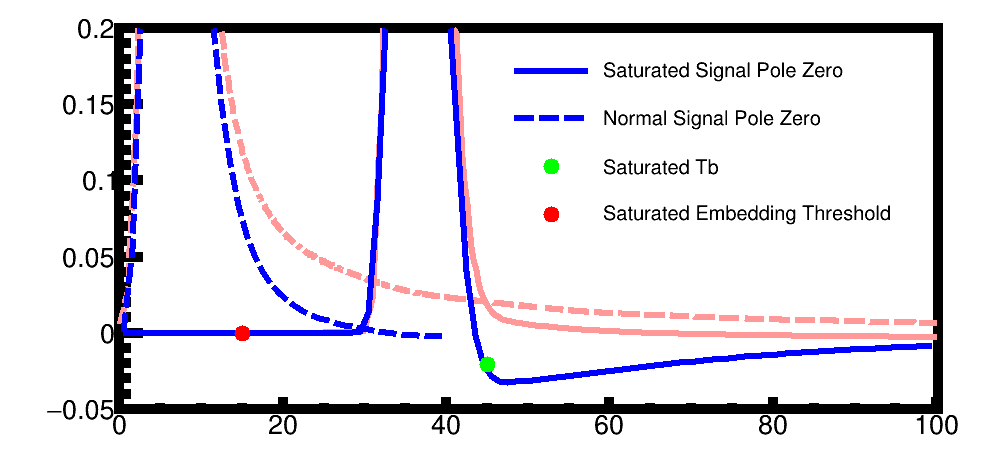
\includegraphics[width=\linewidth]{satpulsepz.png} 
\caption{Pole zero correction} 
\label{fig:pulseSatTag}
\end{figure}


In the case where the input signal is very large, the electronics can be dead for up to \SI{35}{\milli\second} \cite{akiGET}. The beam rate in the experiment was about \SI{10}{\kilo\hertz}, which corresponds to an average of \SI{100}{\micro\second} between subsequent beams. In this case channels can be effectively dead for several events before recovering. Due to the large charge of the beam, a large amount of very high energy electrons --delta rays-- are produced from the beam passing through the gas. In the presence of the magnetic field the radius of curvature of most of the electrons are within several \si{cm} in the xz-plane. Figure~\ref{fig:deltaE} shows the horizontal extent of the delta rays in a top down view of the TPC. While some of the electrons can stop in the gas, some electrons have a high enough kinetic energy going in the vertical direction, penetrating the gating grid without being blocked. They then either terminate on the pad or possibly deposit their charge directly in the pad. The charge induced on the pad is large enough to kill the pad for a time long enough to last until at least the next event. This type of saturation is randomly distributed for pads sitting directly in the beam path and are dead for that event and the next event. 


\begin{figure}[!htb]
    \centering
    \begin{subfigure}[t]{0.49\textwidth}
        \centering
        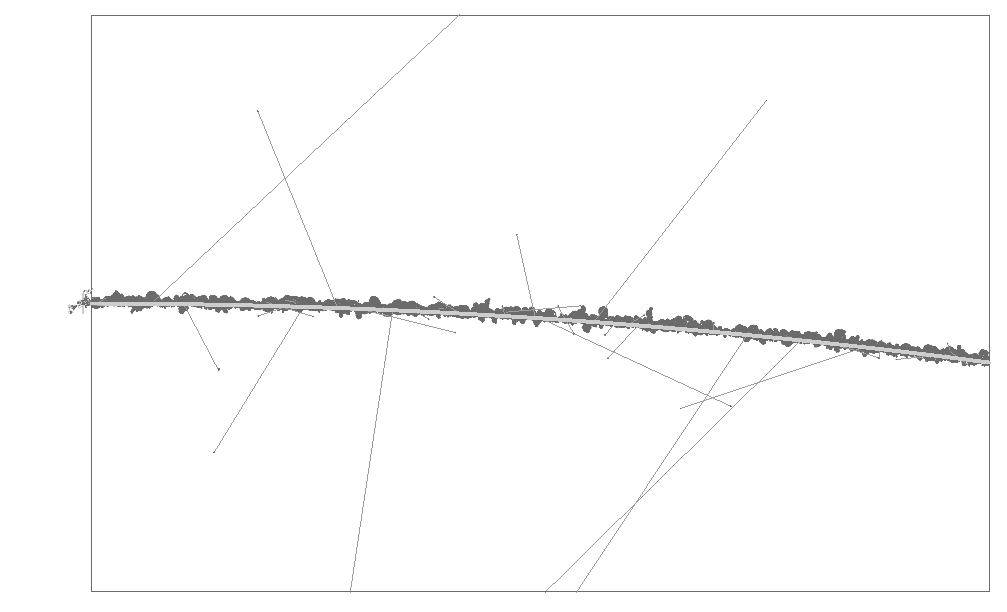
\includegraphics[width=\linewidth]{deltaE_topview_neg} 
        \caption{Top view} \label{fig:deltaE_topview}
    \end{subfigure}
    \hfill
    \begin{subfigure}[t]{0.49\textwidth}
        \centering
        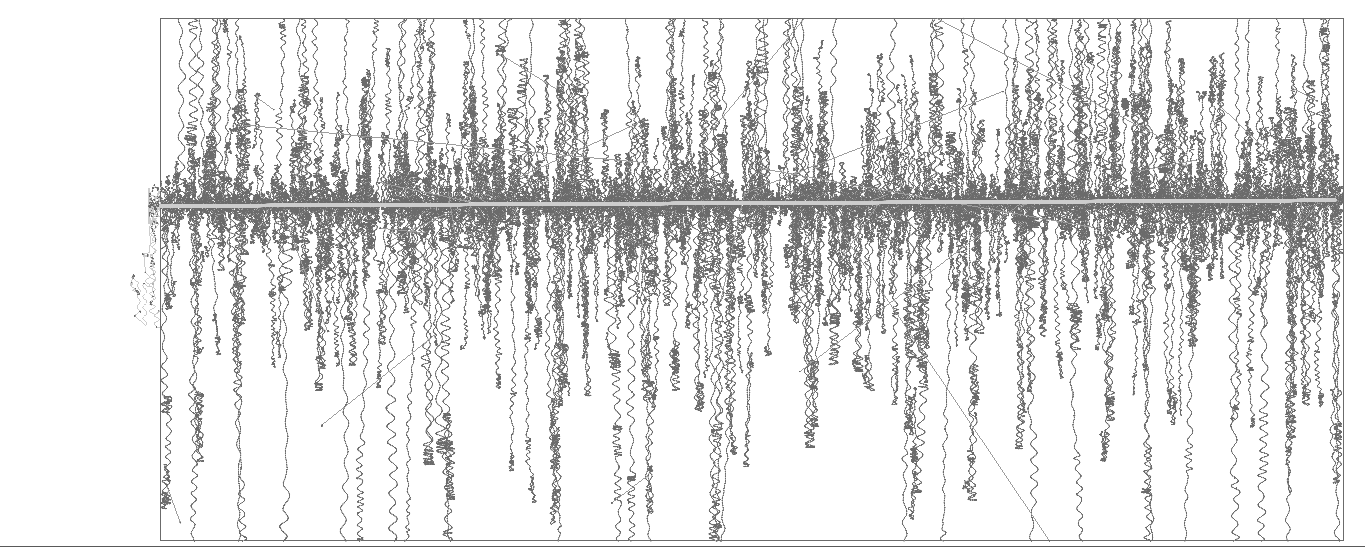
\includegraphics[width=\linewidth]{deltaE_sideview_neg} 
        \caption{Side view} \label{fig:deltaE_sideview}
    \end{subfigure}
    \caption{Geant4 simulation of ${}^{108}$Sn beam at 270 MeV/A in P10 gas. Notice the extent of the delta electrons in the vertical direction as compared to the horizontal extent. }
\label{fig:deltaE}
\end{figure}


\begin{figure}[!htb]
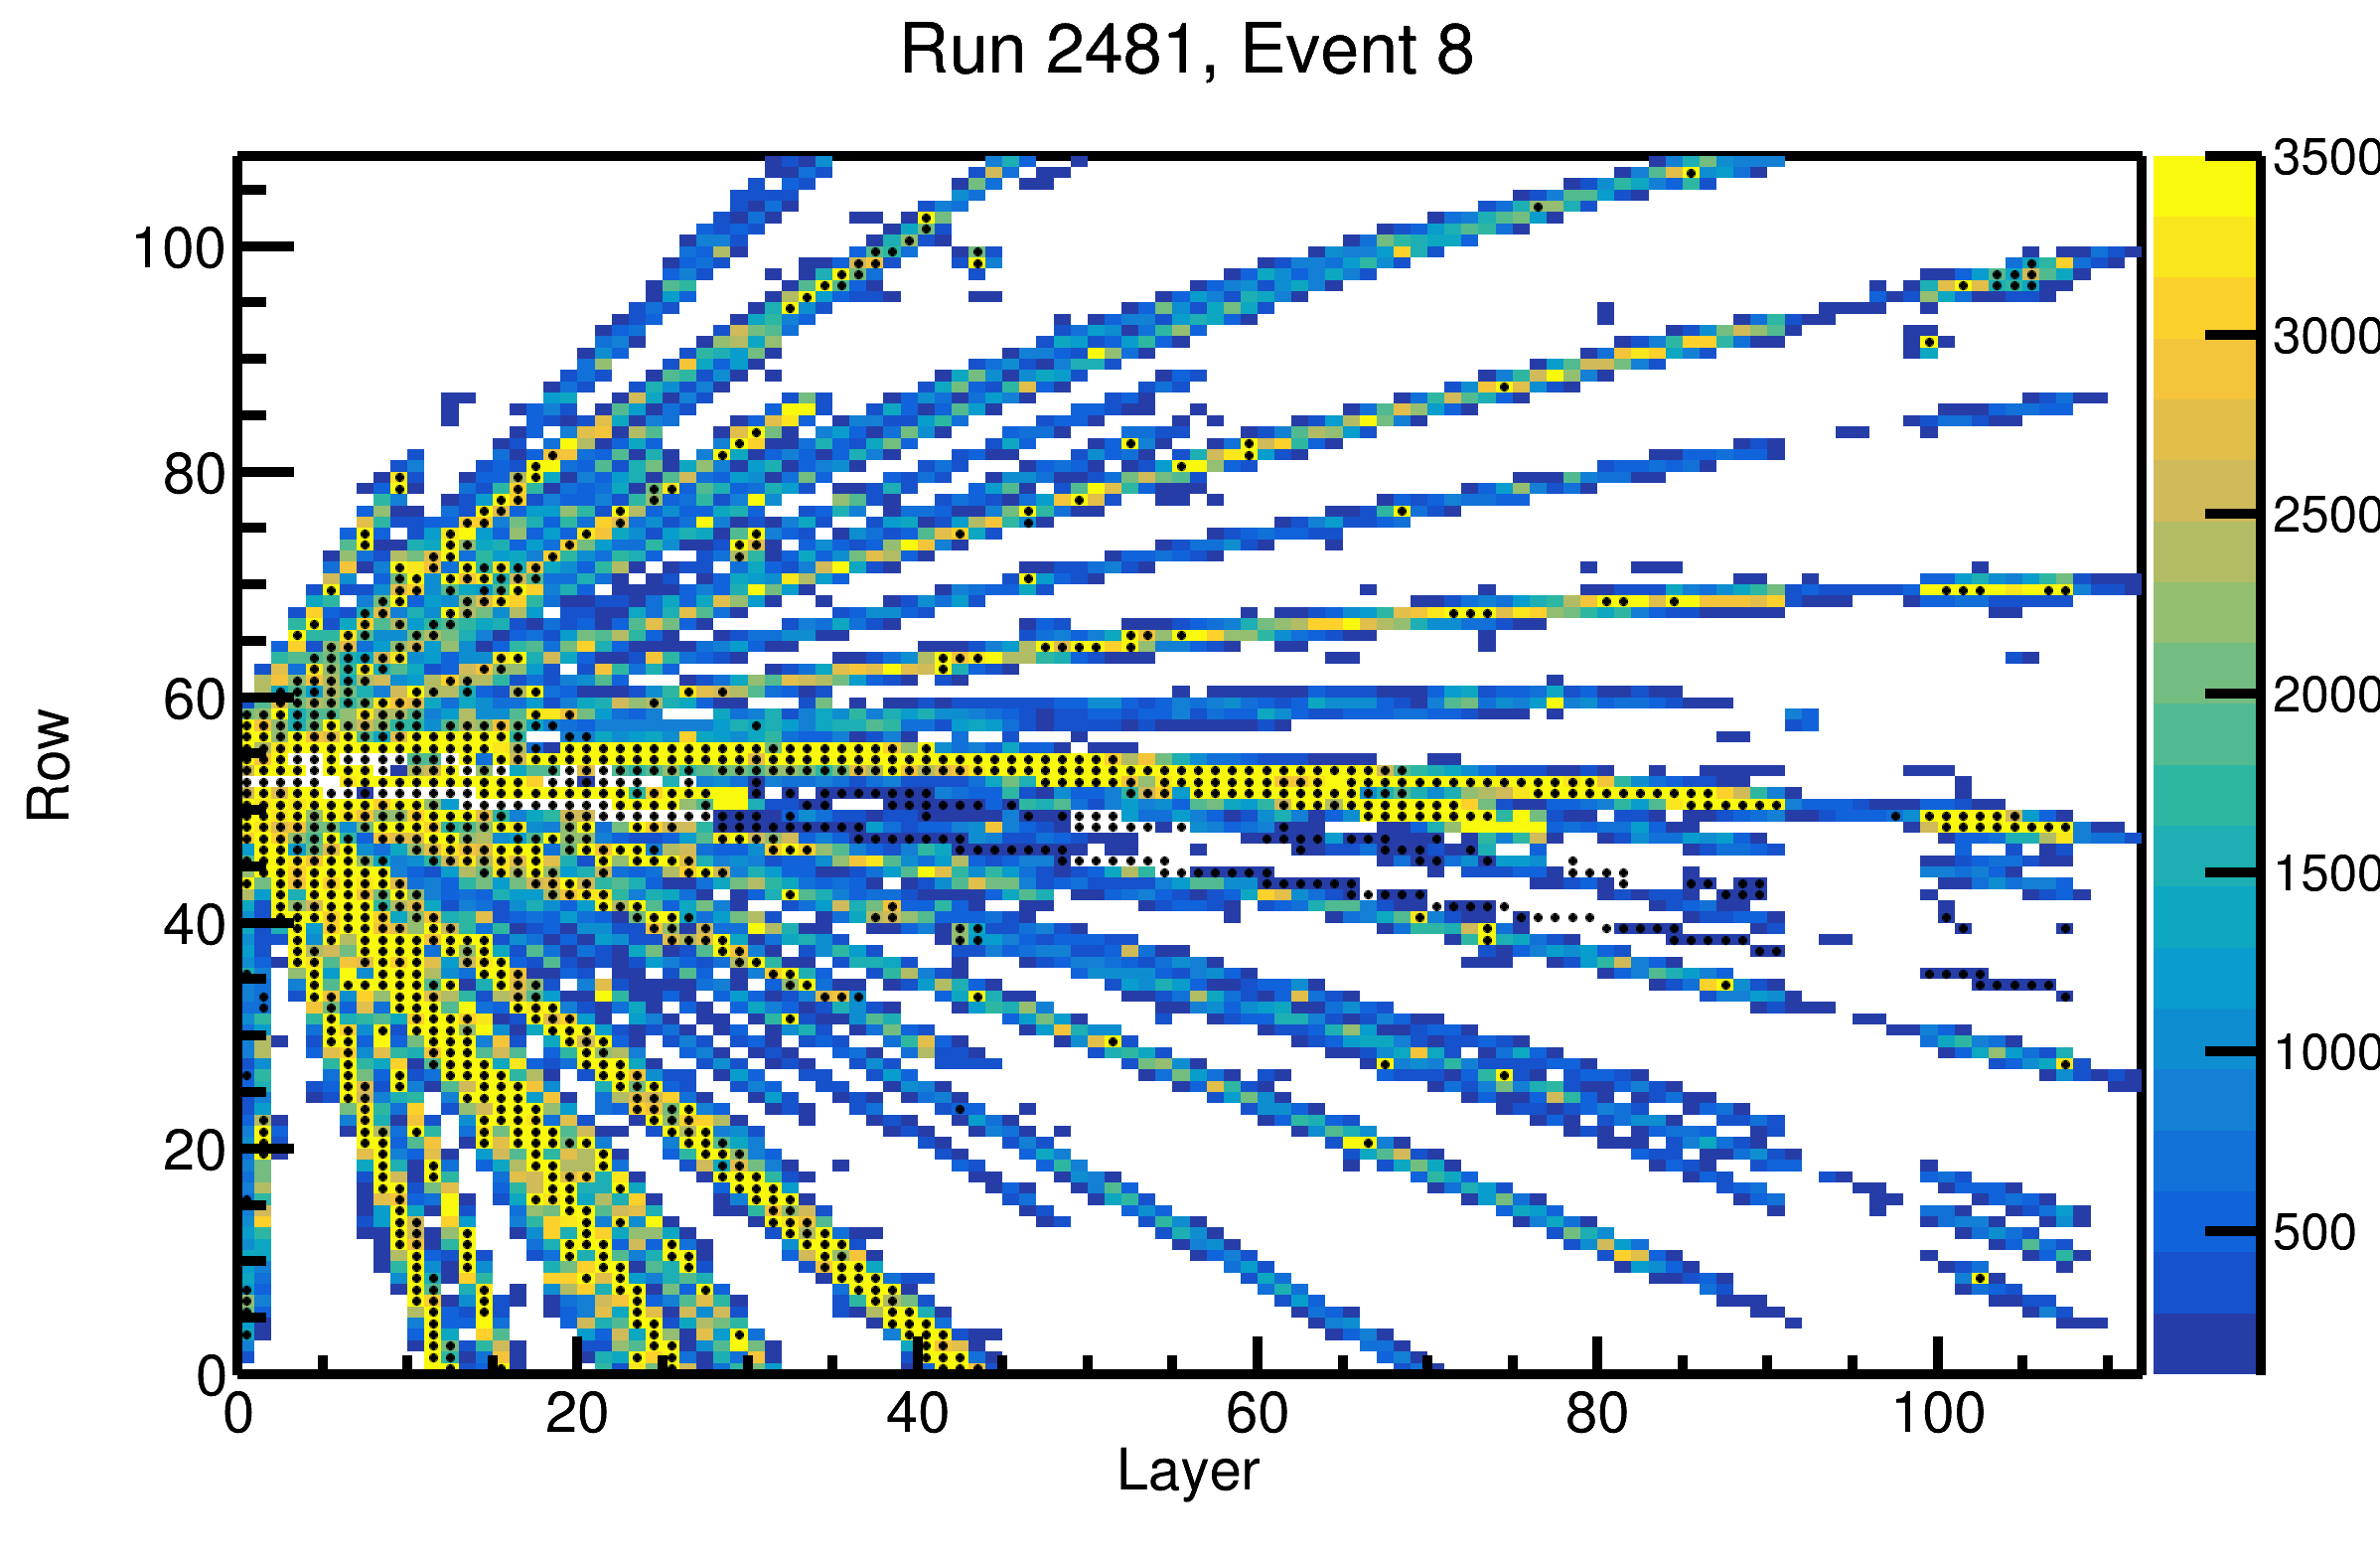
\includegraphics[width=\textwidth]{padplane_sat.png}
\caption{Tagging the saturated pads.}
\label{fig:satTag}
\end{figure}

The simulation of these saturation effects is handled naturally by embedding MC tracks into real data. Once the time bucket of the saturating signal has been identified, no further signals are embedded since the pad is assumed to be dead. In the case a pad is dead for the whole event, the time of saturation is set to the first time bucket and no signal is embedded at all. 

The characteristic signature of a saturated signal is the fast fall time of a pulse, which quickly reaches zero, as opposed to the long tail of normal pulses as seen in Fig.~\ref{fig:pulseshape}. The long exponential tail can be effectively removed by a simple software technique which is similar to the electronics concept of ``pole-zero compensation". If the raw ADC value at a particular time, $i$, is represented as $f_i$, the corrected pulse which differentiates out the exponential tail, $f_i^{'}$ can be expressed as, 

\begin{equation}
f_i^{'} = \frac{-b_1\cdot f_{i-1}^{'} + a_o\cdot f_i + a_1 \cdot f_{i-1}}{b_o}
\label{eq:satpolez}
\end{equation}

where $a_o$ = .9723, $a_1$=-.9453, $b_o$=.9545, and $b_1$=-.9203. These coefficients correspond to the case where the long tail of the standard non-saturating goes to zero, without producing any negative undershoots. In the case of applying this technique to the saturated pulse, the correction produces a negative undershoot since there was no long exponential tail to begin with. Figure~\ref{fig:pulseshape} shows the pulses as the red curves, and after the pole-zero compensation as the blue curves for both the normal and saturated pulses. 

By applying this technique to the real data we can identify whether a pad has a saturating pulse in it and what is the time bucket location by looking for this negative undershoot. A negative peak is identified as a saturated signal if it exceeds the threshold of less than -20$\cdot G$ for more than 8 time buckets and the max ADC value is > $G\cdot$500 where $G$ is the gain calibration of the pad. The max ADC condition eliminates false positives which come from  dead pads where the gating grid subtraction is still applied introducing false negative peaks. The pad is then flagged as saturated and the data time bucket position of saturation is set to $t_{peak} - 5$, where $t_{peak}$ is the time bucket of the negative peak, since the falling edge is around 5 time buckets after the beginning of the saturation. A separate time is also stored called the MC time bucket position which sets the point in time in which a signal cannot be embedded any further. This time is set to $t_{peak} - 30$ to ensure that the MC embedded signals do not overlap the real saturating data signal, which would be impossible. 

Saturation can also occur if of all the pulse heights within the time bucket spectrum add to a value over the max ADC threshold of 3500 ADC. This arises because the fall time of the pre-amplifier circuit is much longer than the time bucket measurement window and pulses are allowed to pile up in the pre-amplifier. In this case no single pulse will reach over the max ADC value yet the last pulse to create saturation will have a pulse shape that has no long tail but otherwise look like a normal pulse. These pulses are also identified by the algorithm described above since there is still no long tail. When embedding tracks into pads, we do not consider the previous amount of total charge in the pad. We assume this method of saturation is a higher order correction and the current algorithm approximates most of the saturation effects which progress through the first process.  Figure~\ref{fig:satTag} shows all of the pads tagged by the algorithm as saturated for an event in the TPC. The max ADC values in a given pad are colored and the black dots represent saturated pads. Some pads appear to be below 3500 ADC, but upon further inspection they satisfy the second process of saturation where the sum is greater than the max ADC value.  

Dead pads are identified earlier in the software in the STCore class. A dead pad is simply a pad which only contains electronic noise and no signals. A dead pad is identified by having a total ADC r.m.s. value  of less than 50 ADC and a max ADC < 50 over the full time bucket spectrum. Here the dead pad is also tagged as saturated and the time bucket position of saturation is set to the first time bucket. 

NEED TO ADDRESS WHY THE MAX ADC THRESHOLD IS 3500
%maybe simple pream fig
%maybe example from aki paper about times
%maybe 

%Add figure showing saturated time bucket spectra with location of saturation identified and with pulse shape from embedding I would like to add and how it blocks it.
%Add Figure with 2D pad plane response with and without saturation flag


\section{Monte Carlo Track Embedding}
\label{sec:embedding}
Track embedding is the process of taking a MC simulated track and embedding its response into an experimental data event. After reconstructing this new embedded event we match the input MC track to the corresponding final reconstructed track.  By doing so we can evaluate the response of the entire TPC system to any given input. The TPC measurement can be thought of three different systems each which introduce errors and or biases into the final reconstructed tracks; the software, the detector, and the experimental setup. The 

There are several effects in a complex experimental set up that influence the data in either unknown or un-quantifiable ways. One such effect is the bias of the triggering system, here the Kyoto and Katana multiplicity and veto arrays preferentially select data that is emitted in a particular reaction plane. As previously discussed saturation effects in the electronics, notably the shadowing of other tracks. The effects of track multiplicity and the distribution of heavy ion and residues from the breakup of the target and projectile. One could propose to make a simulation or investigation into each individual effect in order to make a full MC simulation of data and study the response of the detector this way. Though great care was taken in developing an accurate MC simulation, like all models there are assumptions and simplifications that were made. Simply put, there is no better substitute for experimental data than itself. By embedding MC tracks into experimental data -- and propagating through the tracking and reconstruction algorithm -- one can account for all these sources of biases which are contained in the experimental data, while at the same time measuring the response of the TPC.

As discussed in Section~\ref{sec:software}, the software is composed of several tasks, each of which have the possibility of introducing errors or biases through assumptions made in the tracking algorithm. The detector system introduces errors related to the physical measurement itself which can be addressed through modeling the TPC, and its materials. 

For all of the sources of biases in the TPC, it is clear that a MC type approach to solving for the response of the TPC would be the most practical method. Also by embedding MC events into real data we can take into account the effects of the experimental setup as well as the software and the detector system all together at once. 

%\begin{sidewaysfigure}[H]
%\centering
%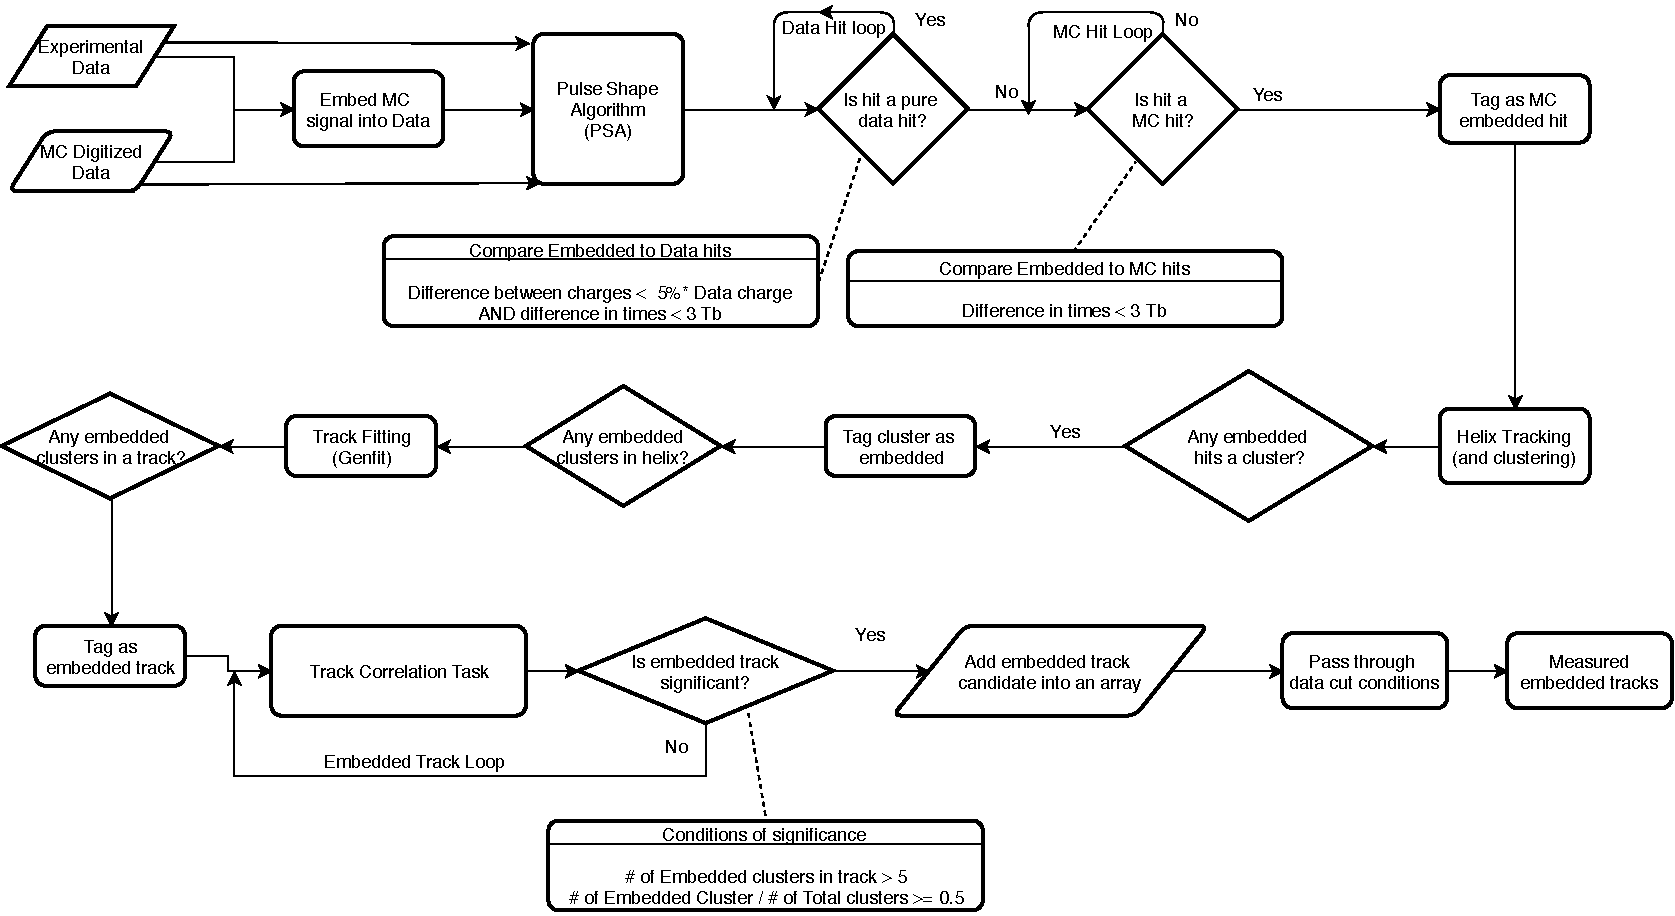
\includegraphics[width=\textwidth]{FlowEmbedding.pdf}
%\caption{Flow of embedding implementation in the software.}
%\label{fig:flow}
%\end{sidewaysfigure}


%\clearpage
%\pagestyle{lscape} % first clear the page and change the pagestyle
%\begin{landscape}
% your landscape table(s) or figure(s) here
%CONSIDER ROTATING THIS FIGURE IF ALLOWED
\begin{figure}[H]
\centering
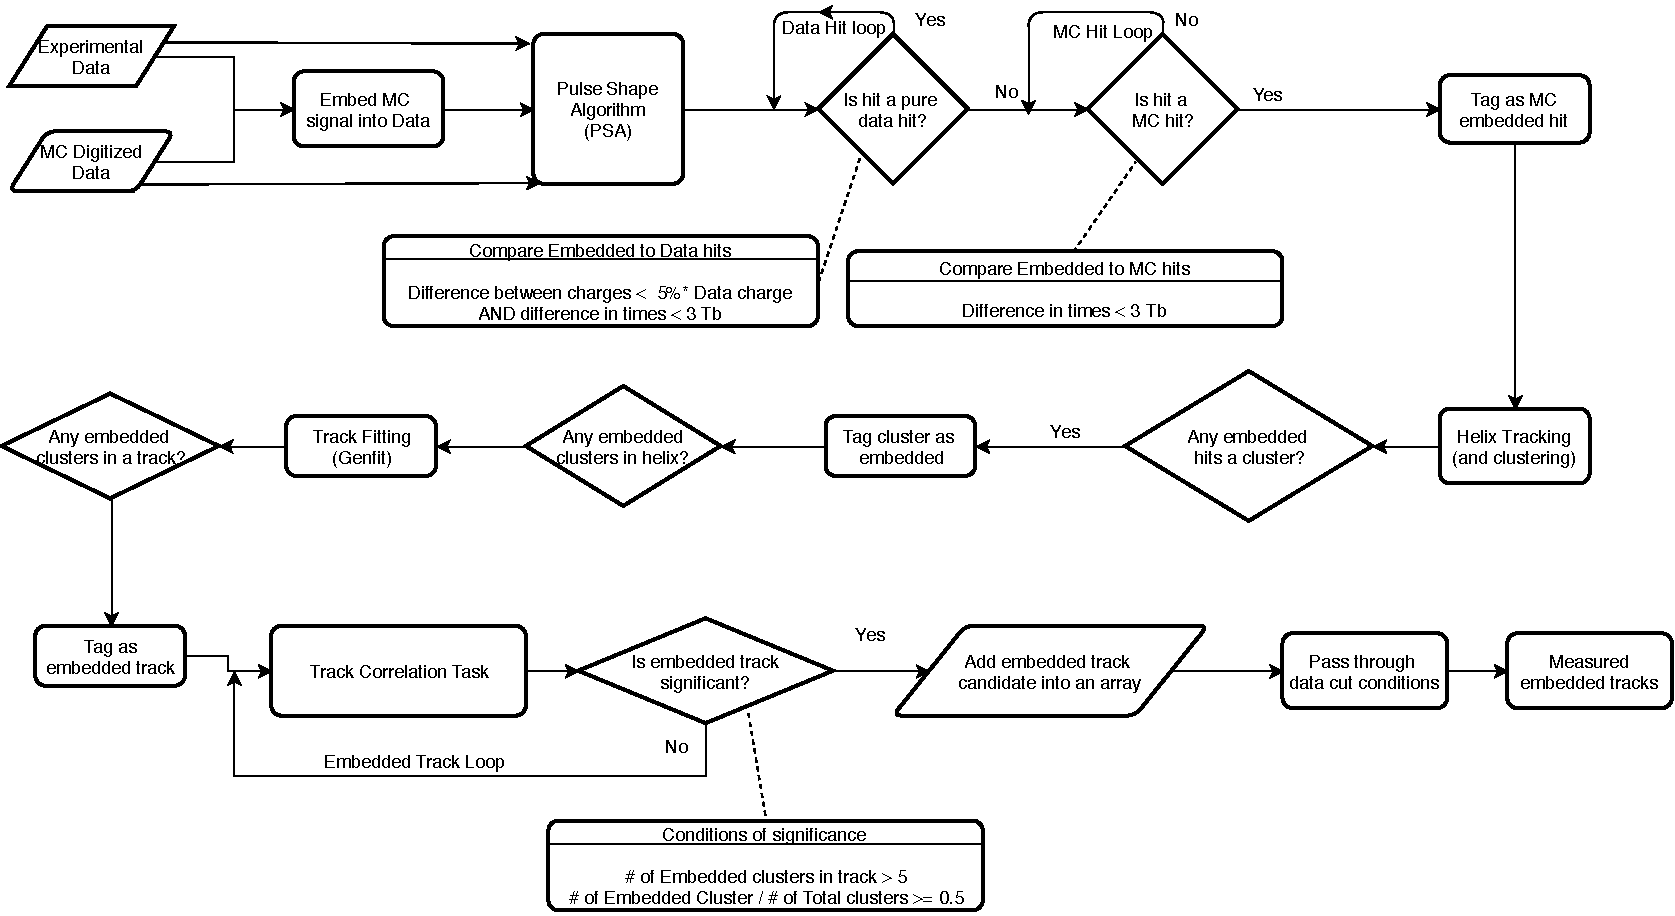
\includegraphics[width=\textwidth]{FlowEmbedding.pdf}
\caption{Flow of embedding implementation in the software.}
\label{fig:flow}
\end{figure}

%\end{landscape}
%\pagestyle{plain}

\begin{figure}[!htb]
    \centering
    \begin{subfigure}[t]{0.49\textwidth}
        \centering
        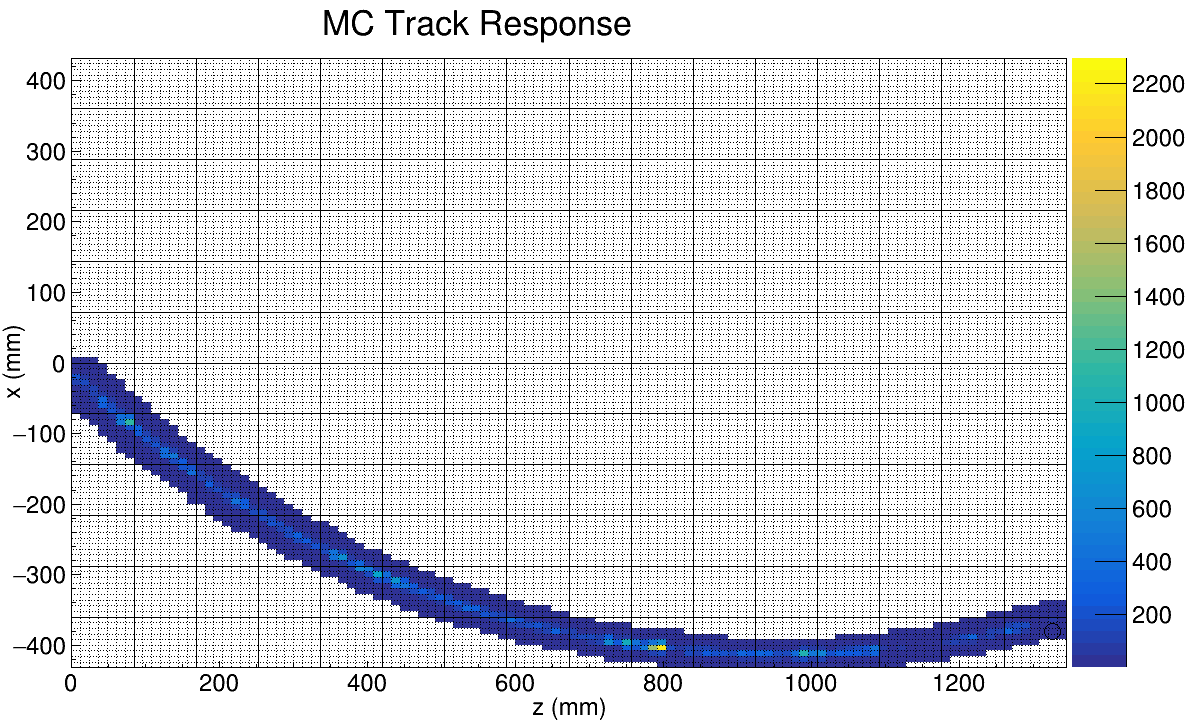
\includegraphics[width=\linewidth]{mcresponse.png}
        \caption{200 MeV/c $\pi^-$ MC digitized track} \label{fig:mcevent}
    \end{subfigure}
    \hfill
    \begin{subfigure}[t]{.49\textwidth}
        \centering
        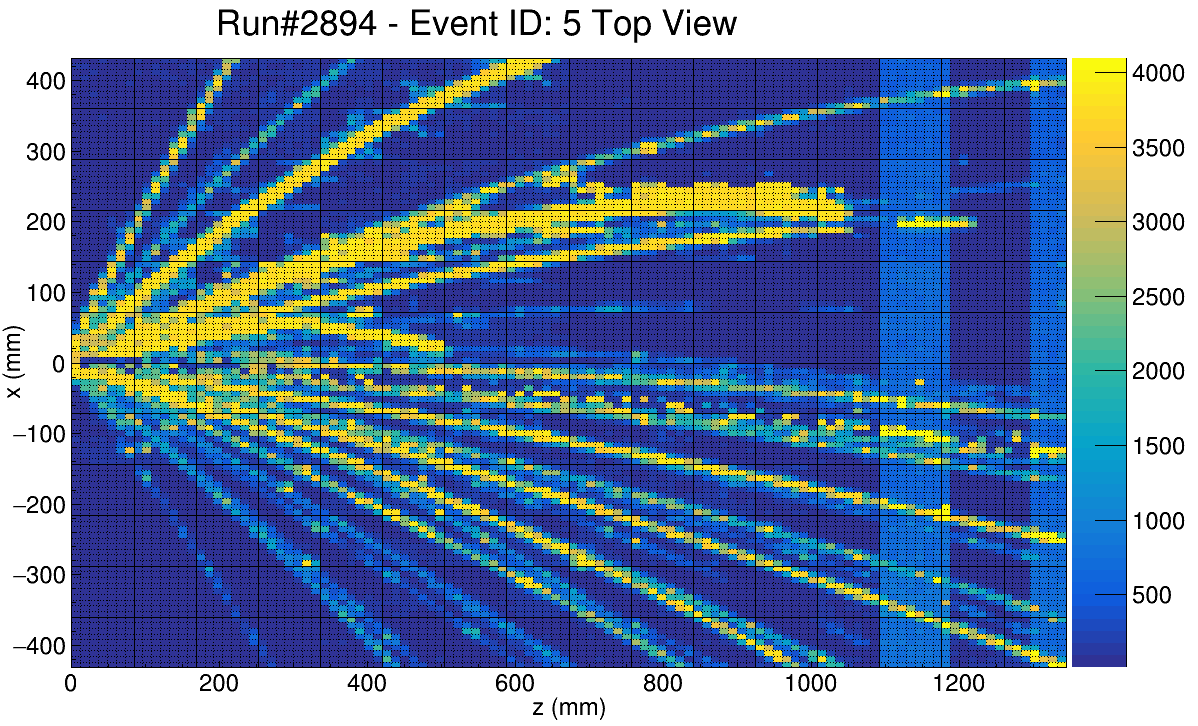
\includegraphics[width=\linewidth]{event5.png} 
        \caption{Experimental data event.} \label{fig:dataevent}
    \end{subfigure}
    \caption{A 200 MeV/c $\pi^-$ embedded into a nuclear collision type event. The embedded track identified by the software is highlighted by the solid green line. }

\label{fig:embedtrack}
\end{figure}



\begin{figure}[!htb]
    \centering
    \begin{subfigure}[t]{0.49\textwidth}
        \centering
        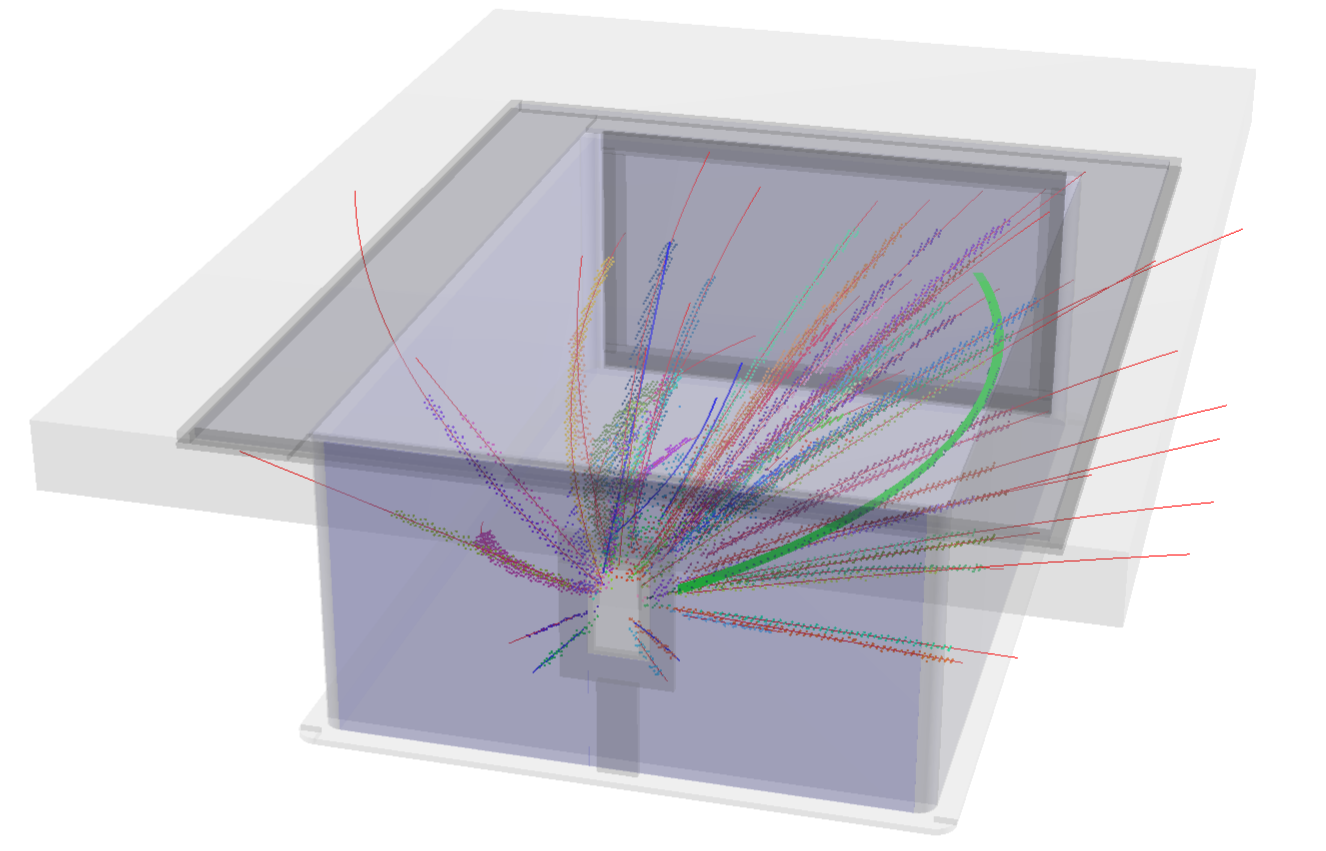
\includegraphics[width=\linewidth]{perspective_embed}
        \caption{Generic} \label{fig:persEmbed}
    \end{subfigure}
    \hfill
    \begin{subfigure}[t]{.3\textwidth}
        \centering
        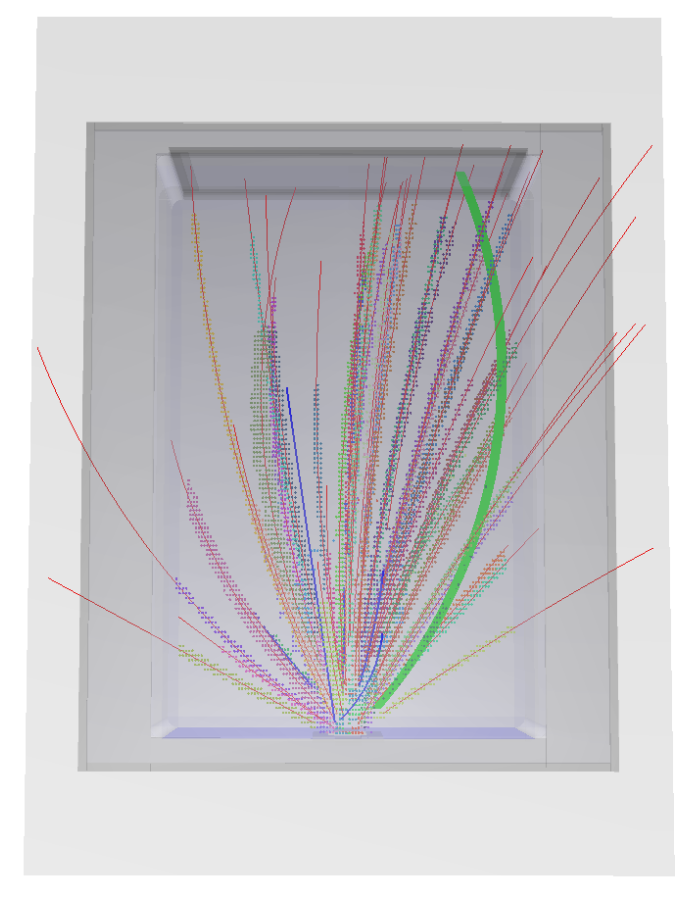
\includegraphics[width=\linewidth]{top_embed} 
        \caption{Competitors} \label{fig:topEmbed}
    \end{subfigure}
     \hfill
    \begin{subfigure}[t]{\textwidth}
        \centering
        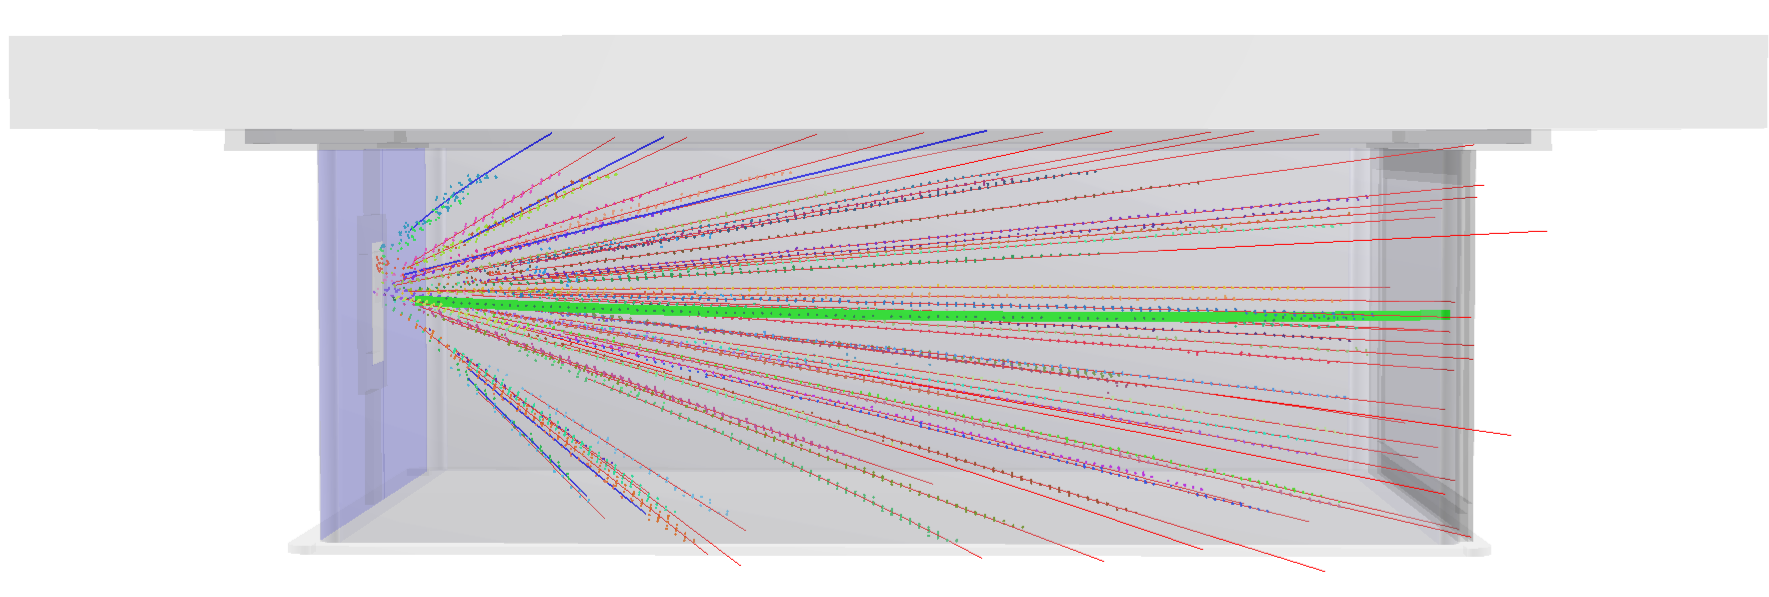
\includegraphics[width=\linewidth]{side_embed} 
        \caption{Competitors} \label{fig:sideEmbed}
    \end{subfigure}
    \caption{A 200 MeV/c $\pi^-$ embedded into a nuclear collision type event. The embedded track identified by the software is highlighted by the solid green line. }

\label{fig:embedtrack}
\end{figure}


The detailed flow diagram of the software implementation of embedding algorithm is shown in Fig.~\ref{fig:flow}. Starting from Geant4 and passing through the 3 MC tasks described above, the output response of the MC track in the TPC is created. From here we directly embed the MC signals into data by adding the MC signals into the data time bucket spectrum, pad-by-pad. As described in Sec.~\ref{sec:simSat}, prior to embedding the MC signals, all pads which are saturated in the experimental data are identified and flagged. The MC signals are forbidden to be embedded after the MC saturation time bucket value. Figure~\ref{fig:mcevent} shows the response of a 200 MeV/c $\pi^-$ track in the TPC; we have embed this track into the data event, Fig.~\ref{fig:dataevent}, just as an example. We will refer to experimental data with embedded MC signals as ``embedded data" for short, the MC generated response as ``MC data", and data only containing only the experimental signals as ``experimental data". The three set of data are each independently analyzed by the PSA algorithm described in Section~\ref{sec:psa},  which finds all the hits associated with each data set. From this the three independent hit data sets are temporarily stored. 

Here within the PSA algorithm, is the first and most important part of the embedding software. The PSA task has the job to identify which hits in the embedded data set originate from the MC hits set and which are from the experimental data. Once the MC hits are identified, these embedded hits can be tagged and tracked through the entire software. 

First, the hits in the embedded set are matched against the experimental data, identifying which of the embedded hits originate from the experimental hit set. For two hits to match, they must satisfy two criteria, $\left|(Q_{\mathrm{Data}} - Q_{\mathrm{Embed} })/Q_{\mathrm{Data}}\right| < .05$ and $\left|t_{\mathrm{Embed} } - t_{\mathrm{Data} }\right| < 3$ where $Q$ and $t$ represent the charge and time of the hit respectively. Hits that satisfy these criteria are then removed from the embedded data set.

The surviving hits are then compared with the MC hit data set, where the criteria for a matching MC hit is, $\left|t_{\mathrm{Embed} } - t_{\mathrm{MC} }\right| < 3$.  There is no requirement for a matching criteria for the charge values which would artificially bias the charge values selected depending on our cut; which is critical for minimum ionizing particles such as pions.  This can only be accomplished by first removing almost all of the experimental hits as was done in the first step. Each embedded hit that passes this step of criteria is tagged as a originating from a MC hit. From here, the embedded data is treated as if it were real data passing through the same software analysis. 

 If a helix track has one hit that is embedded it will also be tagged as embedded. When the hits in a helix track are clustered, if a cluster contains one embedded hit it is itself tagged as an embedded cluster. Furthermore, if a track that is reconstructed contains any embedded clusters, it is tagged as an embedded track. The goal of this na\"ive tagging approach is to preserve all the information of where the embedded hits, clusters, and tracks have gone, preserving as much information until the end without introducing a bias.
 
  It is the job of the embedded correlation task to identify which of the final embedded tracks are candidates for the original input track. For example, several things may happen along the process of embedding that may disqualify a track as a candidate in this na\"ive tagging. A track could break up, lose or share its charge with and adjacent track; it may be not be identified at all for a variety of other reasons. For the embedded track to be a candidate of the input MC track, it must satisfy two conditions, $N_{sat} > 5$ and $N_{\mathrm{sat}}/N_{\mathrm{Total}} \geq .5$, where $N_{\mathrm{sat}}$ is the number of saturated clusters in a track, and $N_{\mathrm{Total}}$ is the number of total clusters. The first criteria is a simple minimum cut where to ensure the minimum condition of a embedded track is met at least having 5 clusters. The second criteria is the strongest cut, ensuring the track has at least half of its clusters coming from embedded MC signals. The set of tracks which satisfy both conditions are saved into an array of candidate tracks. In this way the user can decide how to sort these tracks for studying either efficiency or track splitting. 

If the embedded track is split into multiple tracks, the user must select what they believe to be the track which most represents the original track, for the purposes of calculating efficiency. Typically only one of the tracks in the set will satisfy one of the reasonable quality cut conditions in an analysis. For example the most reasonable assumption is the track originating from the vertex is the most correct in this case, where as the split fraction of the track wont originate from the vertex but instead have a large distance to vertex value. In this thesis, the track with the minimum distance to vertex is identified as the track in which the efficiency analysis will be performed.


\subsection{MC and Data Comparison}

Here we compare several important observables to ensure the MC is simulating the data. These observables will be relevant for the quality cuts and efficiency analysis discussed in Section~\ref{sec:efficiency}. The most important observable is the total number of clusters. The number of clusters in a track depends on the geometry of the TPC, the spherical angles of the track, and the clustering algorithm. MC tracks were embedded into data for several particle types; the input angular and momentum distribution was uniform and the final distributions were weighted such that the angular and momentum distribution matched that of the data for a fair comparison. Figure~\ref{fig:clustcomp} shows the normalized cluster distributions for the MC and data for several particle types. There is no data below 20 clusters because this is the minimum cut to ensure quality PID lines in the data. The normalization is changed for each particle type to display them on the same scale. Very good agreement is seen between the MC and data over a wide range of particle species. 

\begin{figure}[!hbt]
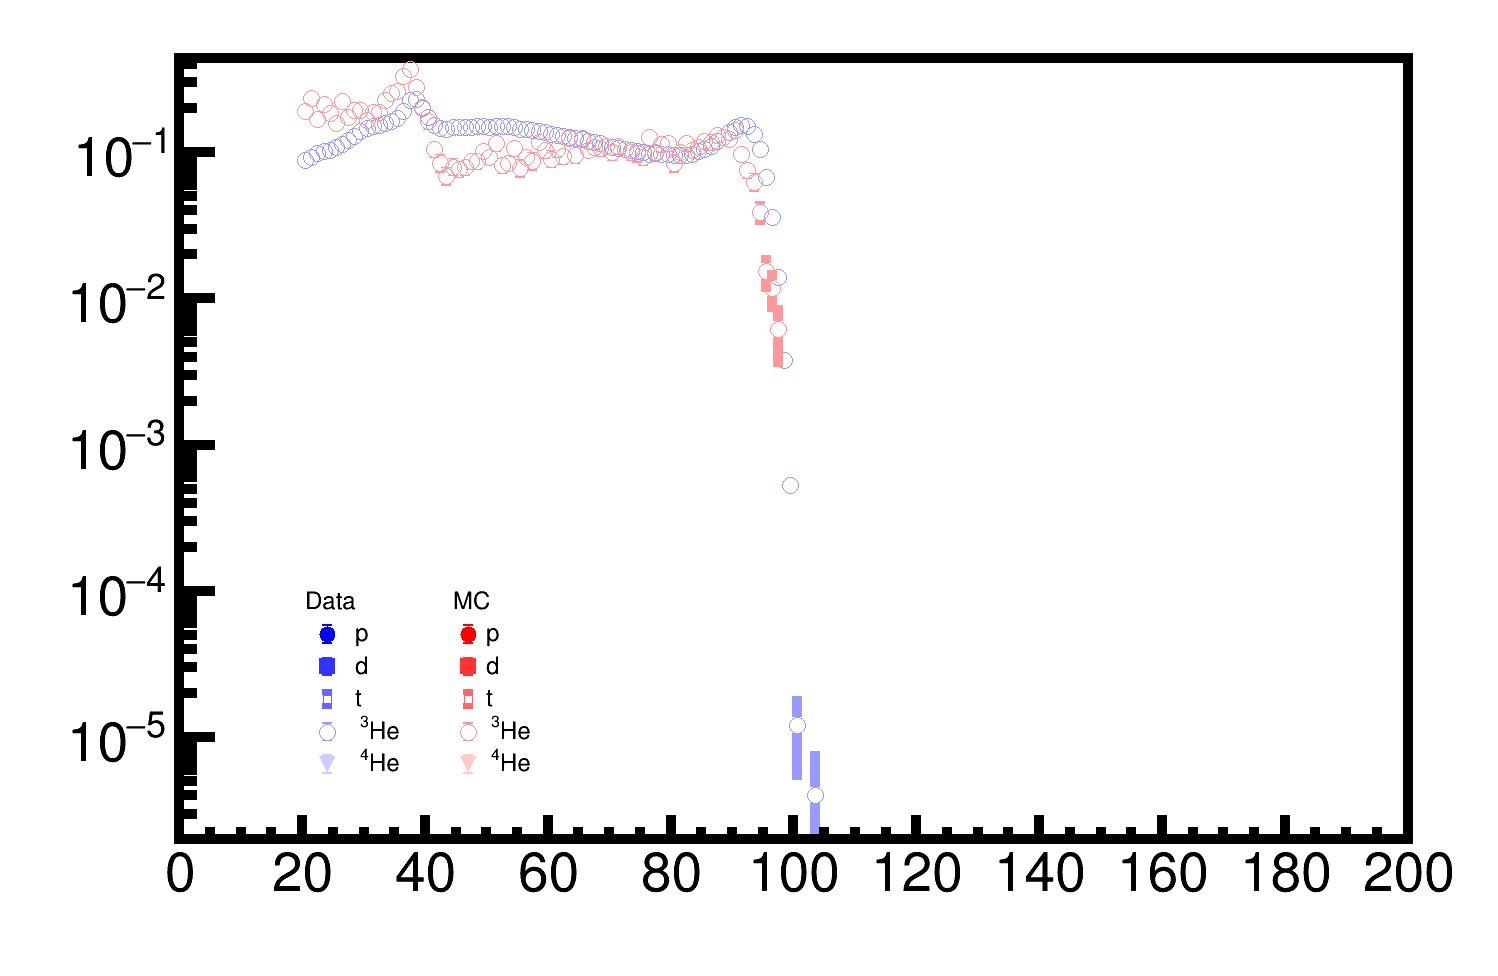
\includegraphics[width=\linewidth]{numcluster.png}
\caption{Comparison of MC to data.}
\label{fig:clustcomp}
\end{figure}

The second most important observable is the distance to vertex. Figure~\ref{fig:pocacomp} shows the distance to vertex distributions for the MC embedded tracks and the data for the same range of particle species. The distributions were again normalized to different values to display on the same scale. Both data sets here are track number of clusters > 20. It is also worth mentioning the data plotted is also after the space charge correction. Before the space charge correction the distributions would be much wider. Since we correct for the space charge in the data we compare here to the embedded MC without any space charge effects, making a fair comparison. 

\begin{figure}[!hbt]
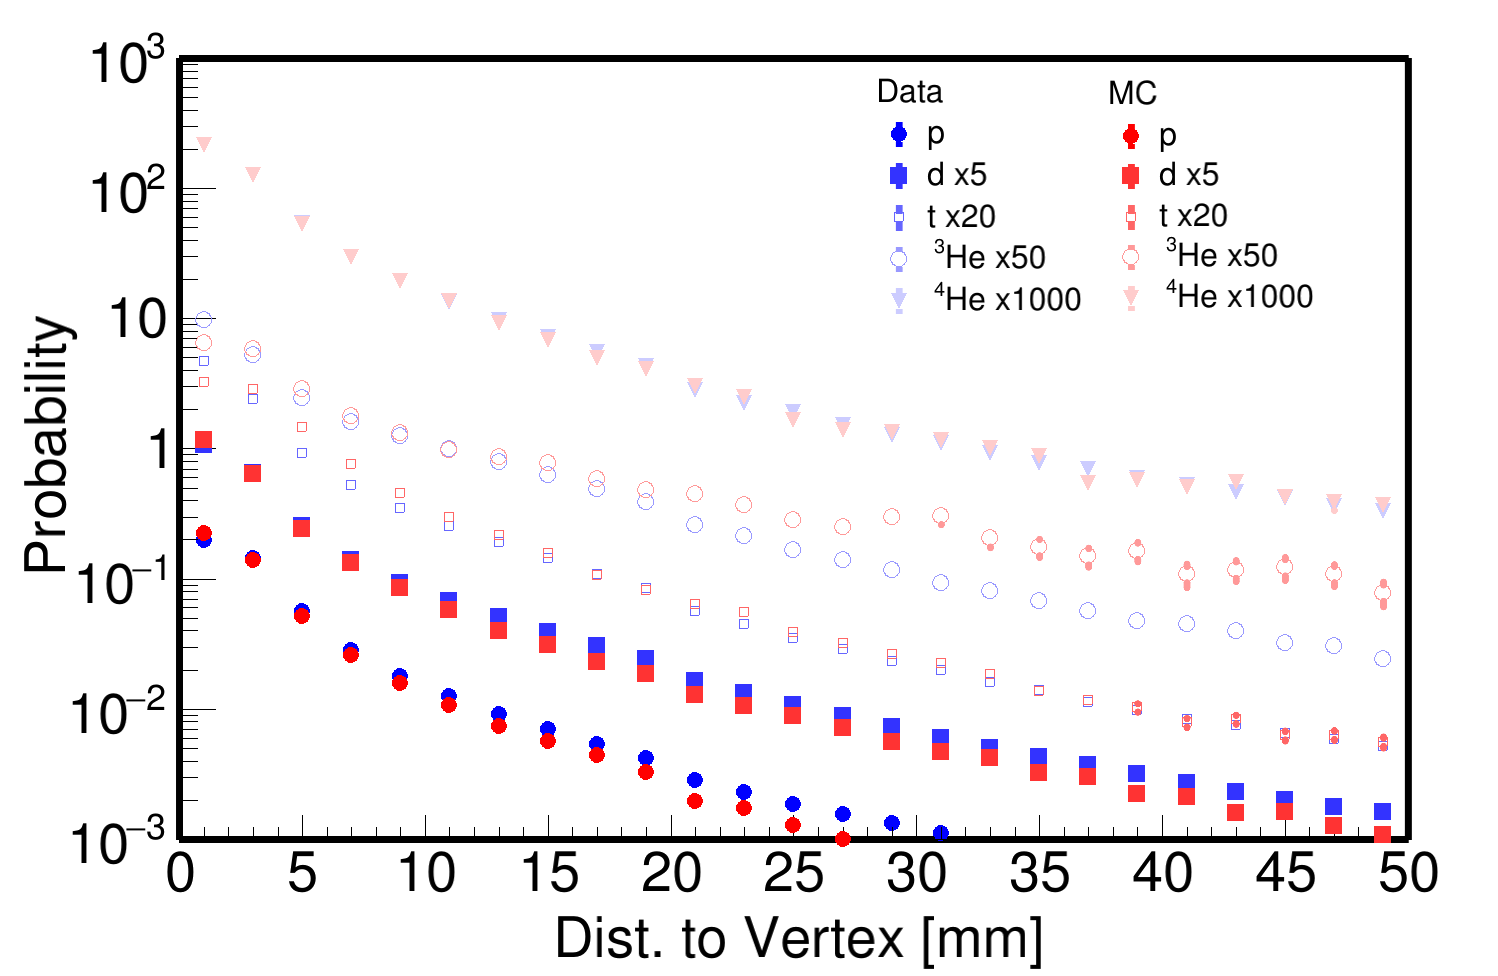
\includegraphics[width=\linewidth]{poca.png}
\caption{Comparison of MC to data.}
\label{fig:pocacomp}
\end{figure}


We can see good agreement between the MC PRF for $\pi^-$ in Figure~\ref{mcdataPRF}, and the data PRF, Fig.~\ref{prfpimData}, where the black line is the PRF fit to the experimental data. It is sufficient to use such a simple universal PRF function as we can describe all the crossing angle effects discussed in \ref{sec:prf}. Therefore these effects must arise from geometric effects related to the track angle, the amount of charge distributed over an anode wire, and the superposition of the PRF from neighboring anode wires which contribute to the appearance of a changing PRF.

\begin{figure}[!htb]
         \centering
         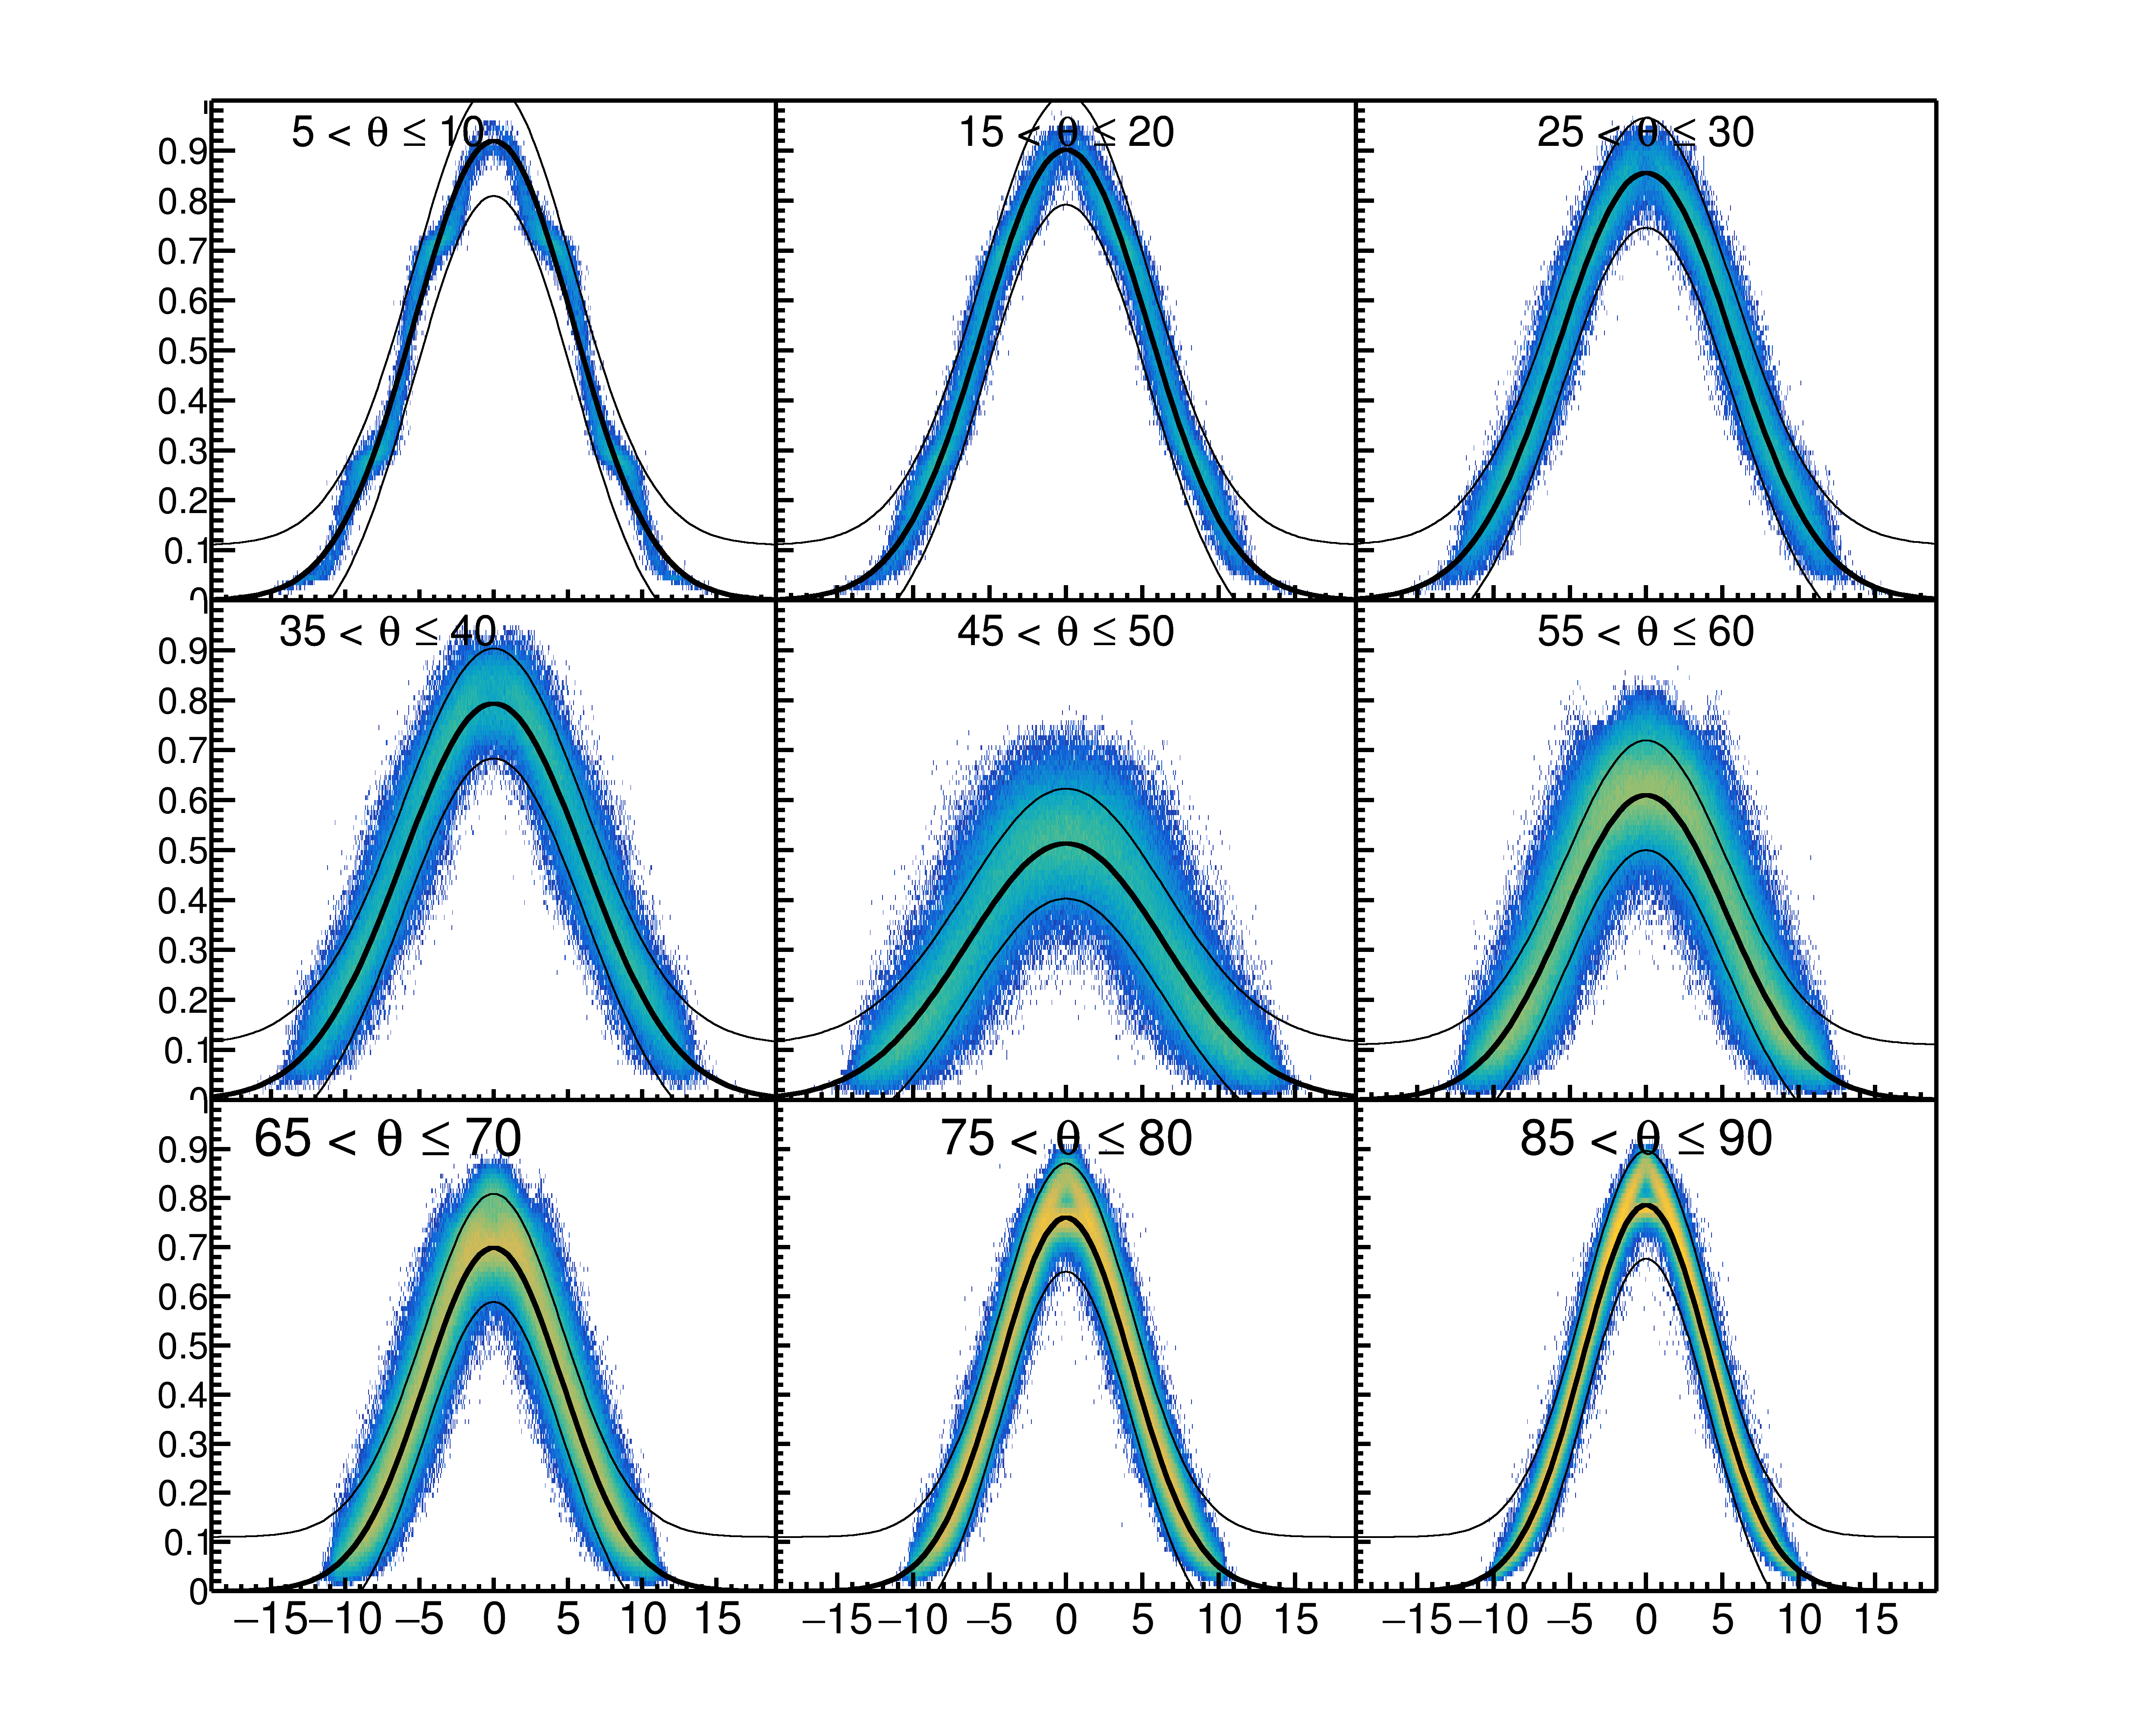
\includegraphics[width=\textwidth]{PRFs_MC_wcut.png}
         \caption{PRF response of Monte Carlo simulation of $\pi^-$}
         \label{fig:prfpimMC}
\end{figure}


%Add Figure of Pad response function for pion,proton.... for MC vs Data vs angles...
%Add Figure of Number of clusters of MC vs Data
Add Figure of dEdx MC vs Data
Add Figure of Momentum resolution MC vs Data
Add Figure of track residuals? MC vs data?


\section{Aligning TPC}

%explain the different shifts in the TPC
%BDC shift
%Hit offshet shift



\section{CoBo timing correction}

The arrival time of signals originating from each pad may differ due to timing delays in the electronics and cabling. The timing differences will affect the y-position measurement of each track. The y-residuals reveal that the timing differences correspond to about $\pm$\SI{2}{\milli\metre} in position differences. The timing difference is stable for each pad across several runs. Figure~\ref{fig:coboCorr} shows the y-residuals, across all the rows , for three different layers. Before the correction one can see large deviations in the y-residuals which correspond to timing differences. The mean value of the y-residual distribution is fitted and a map is constructed for each pad. The data is then reconstructed subtracting the value of that map, $dy$, for each pad. The resulting corrected distribution is shown in Fig.~\ref{fig:coboCorr} for the same layer set. Figure~\ref{fig:yoff} also show the summary of all the pads before the correction and after the correction. There is a significant improvement in the width of the distribution going from \SI{1.5}{\milli\metre} to \SI{0.6}{\milli\metre}. 

\begin{figure}[!htb]
  \begin{center}
    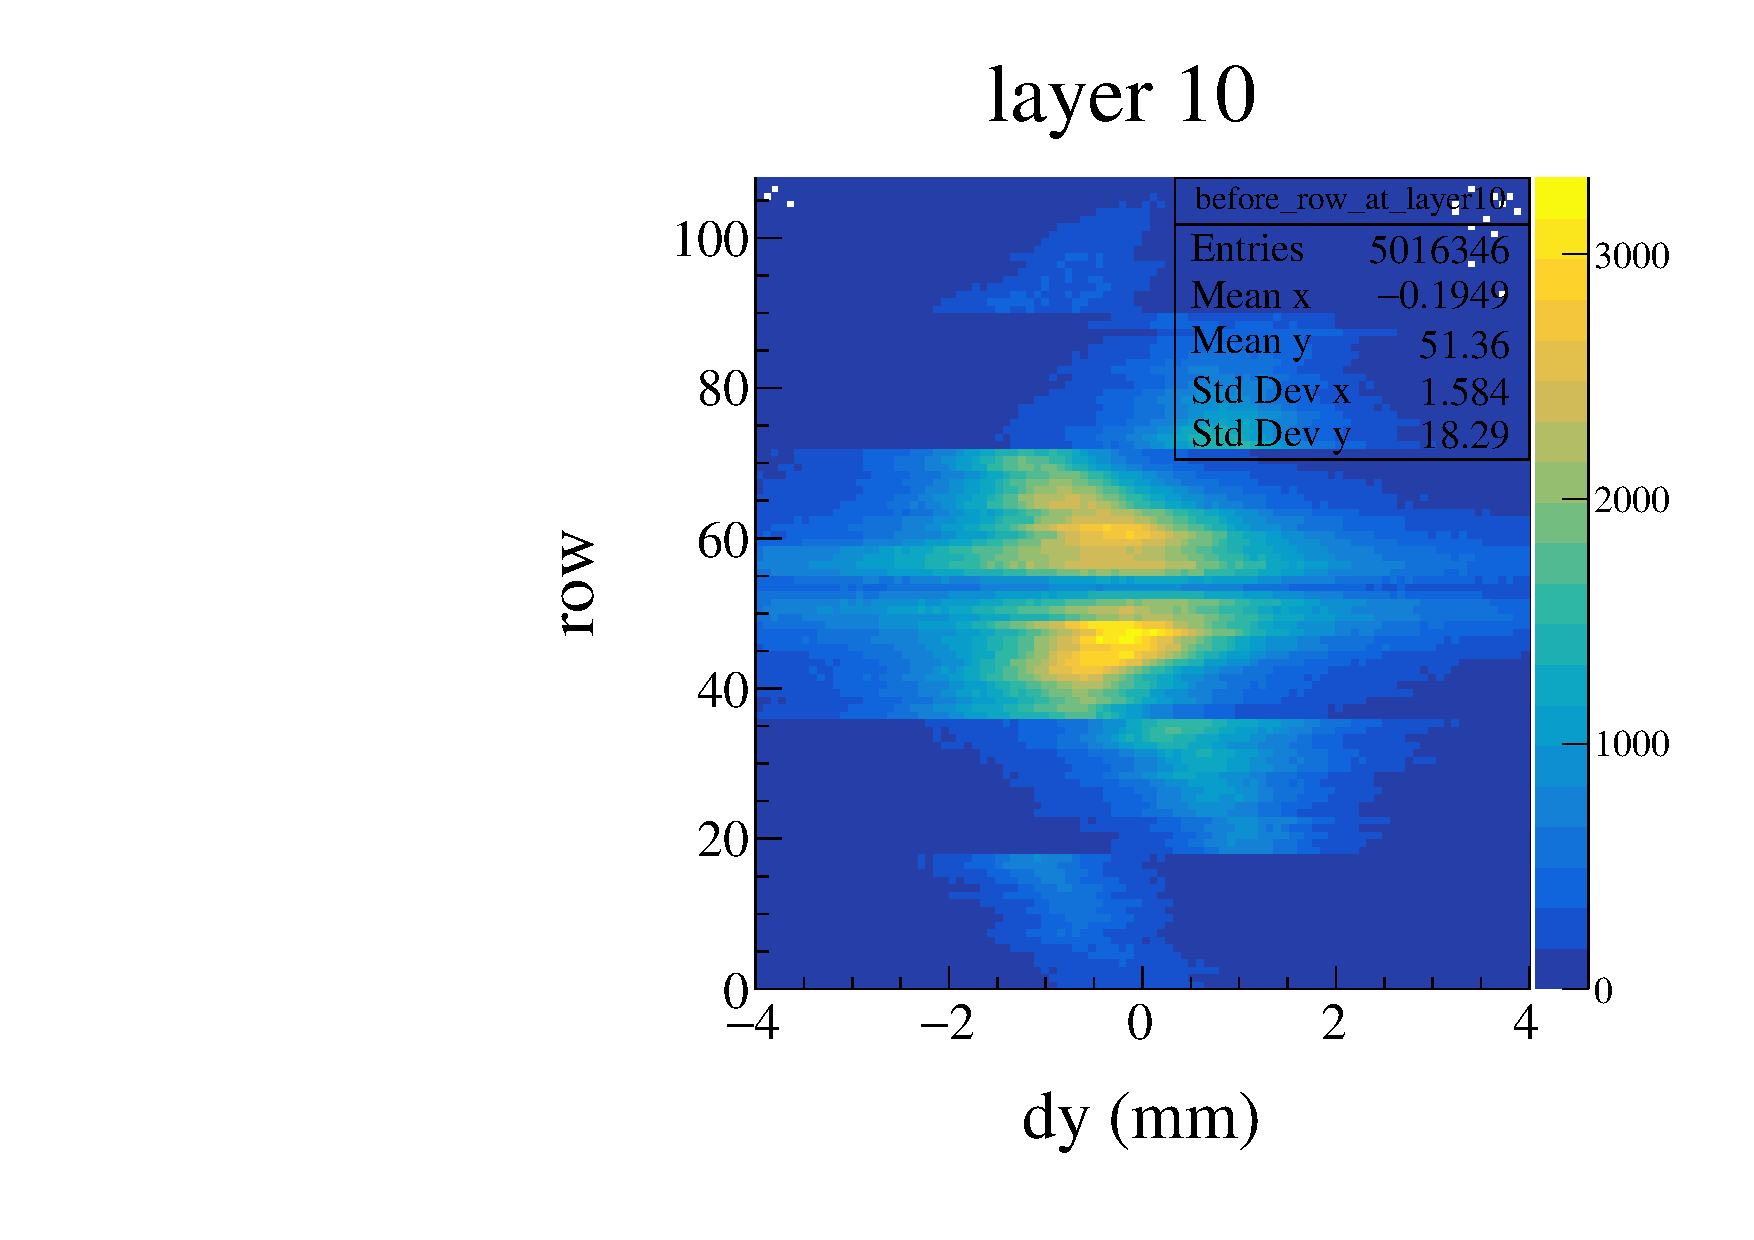
\includegraphics[width=0.33\textwidth]{before_row_at_layer10_yoffset.pdf}
    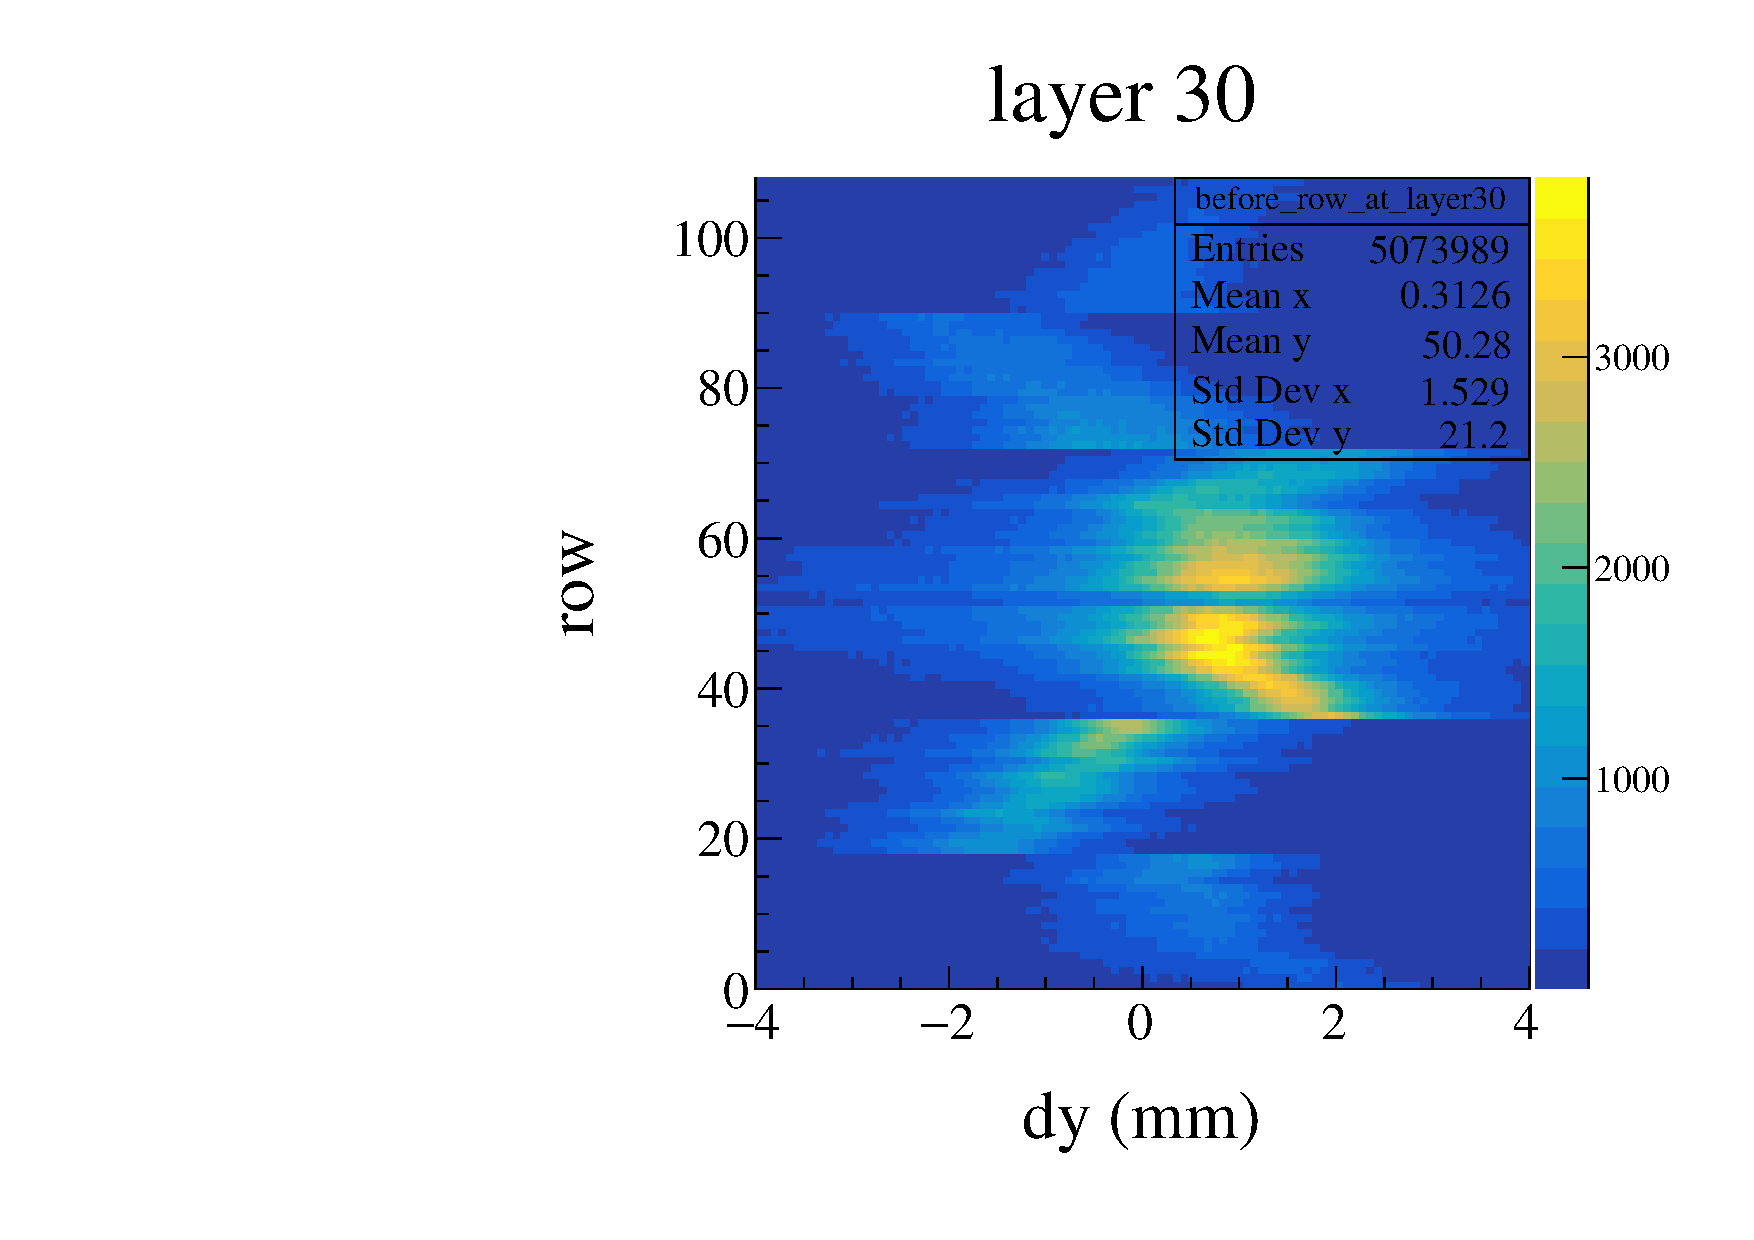
\includegraphics[width=0.33\textwidth]{before_row_at_layer30_yoffset.pdf}
    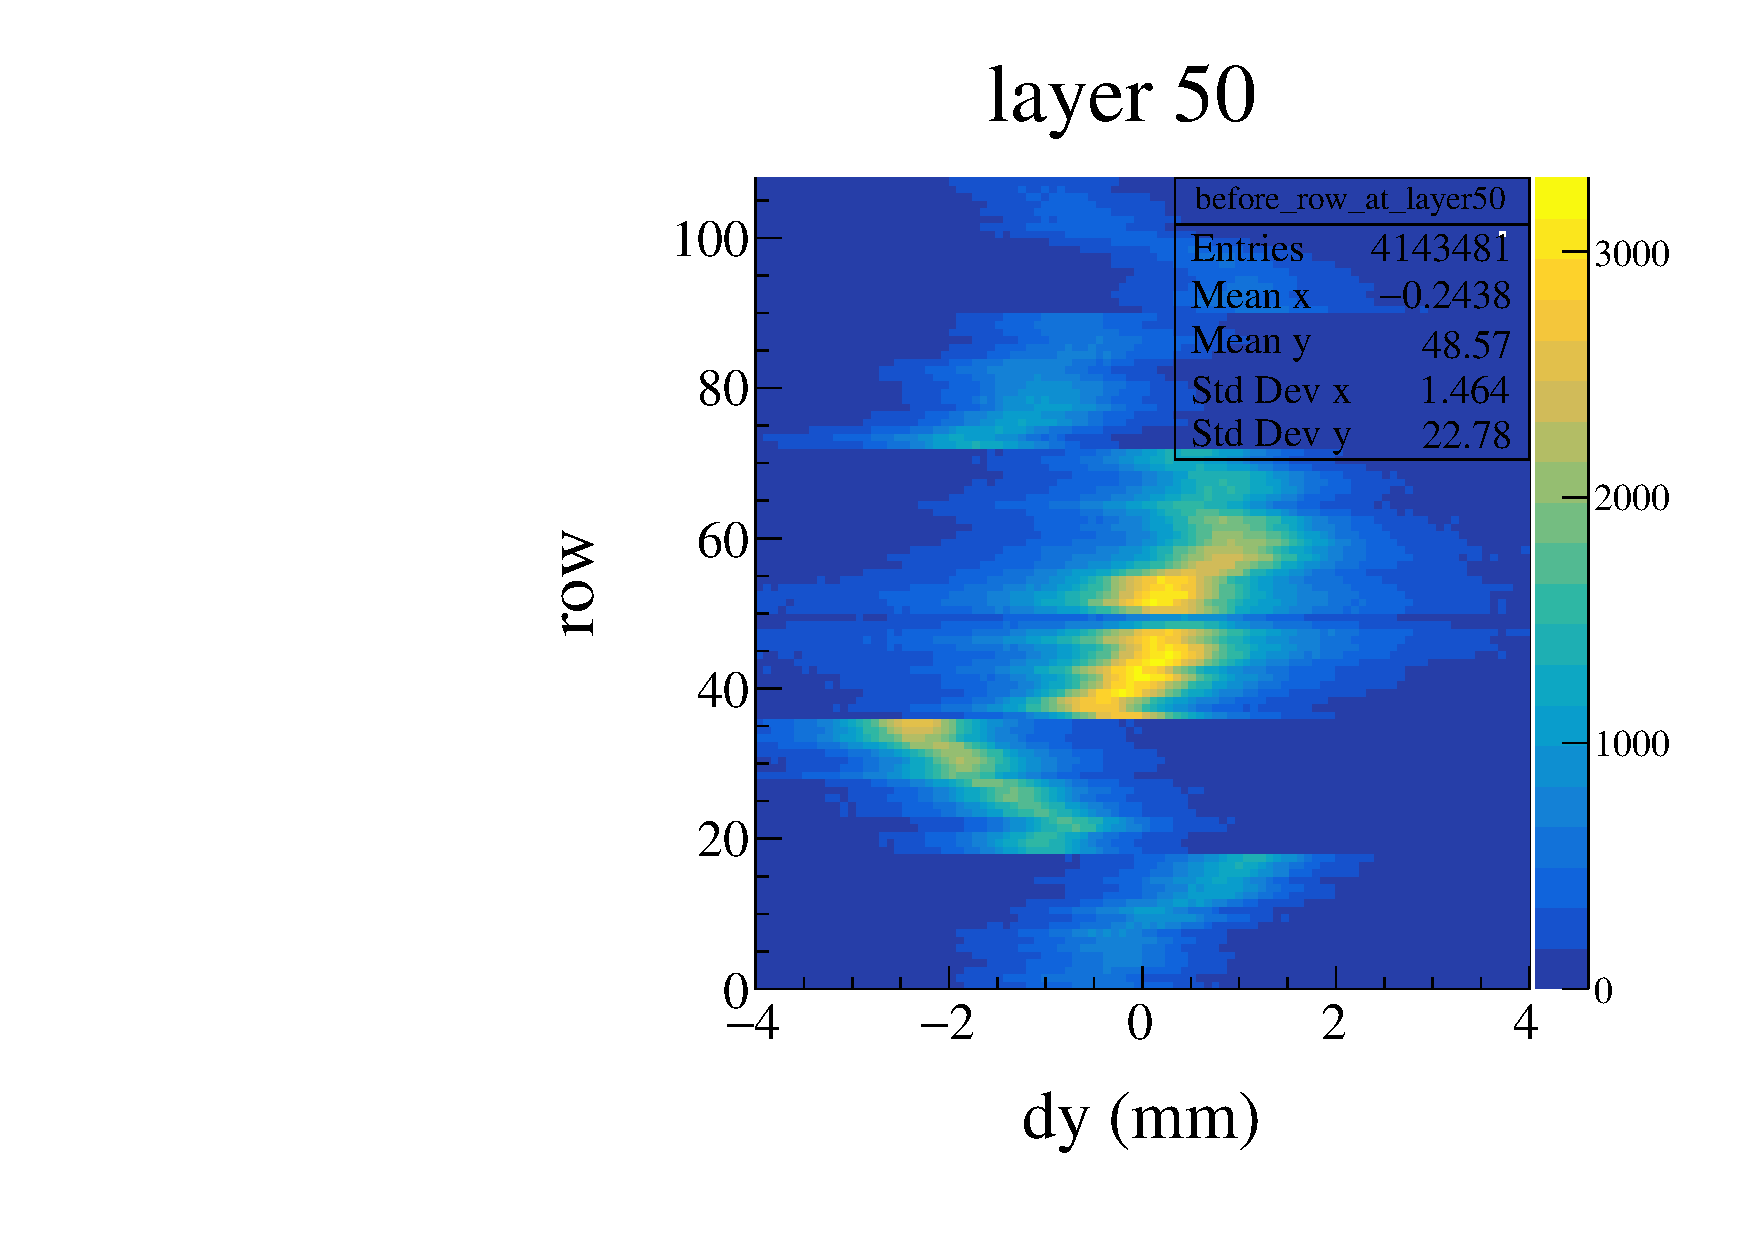
\includegraphics[width=0.33\textwidth]{before_row_at_layer50_yoffset.pdf}
 
    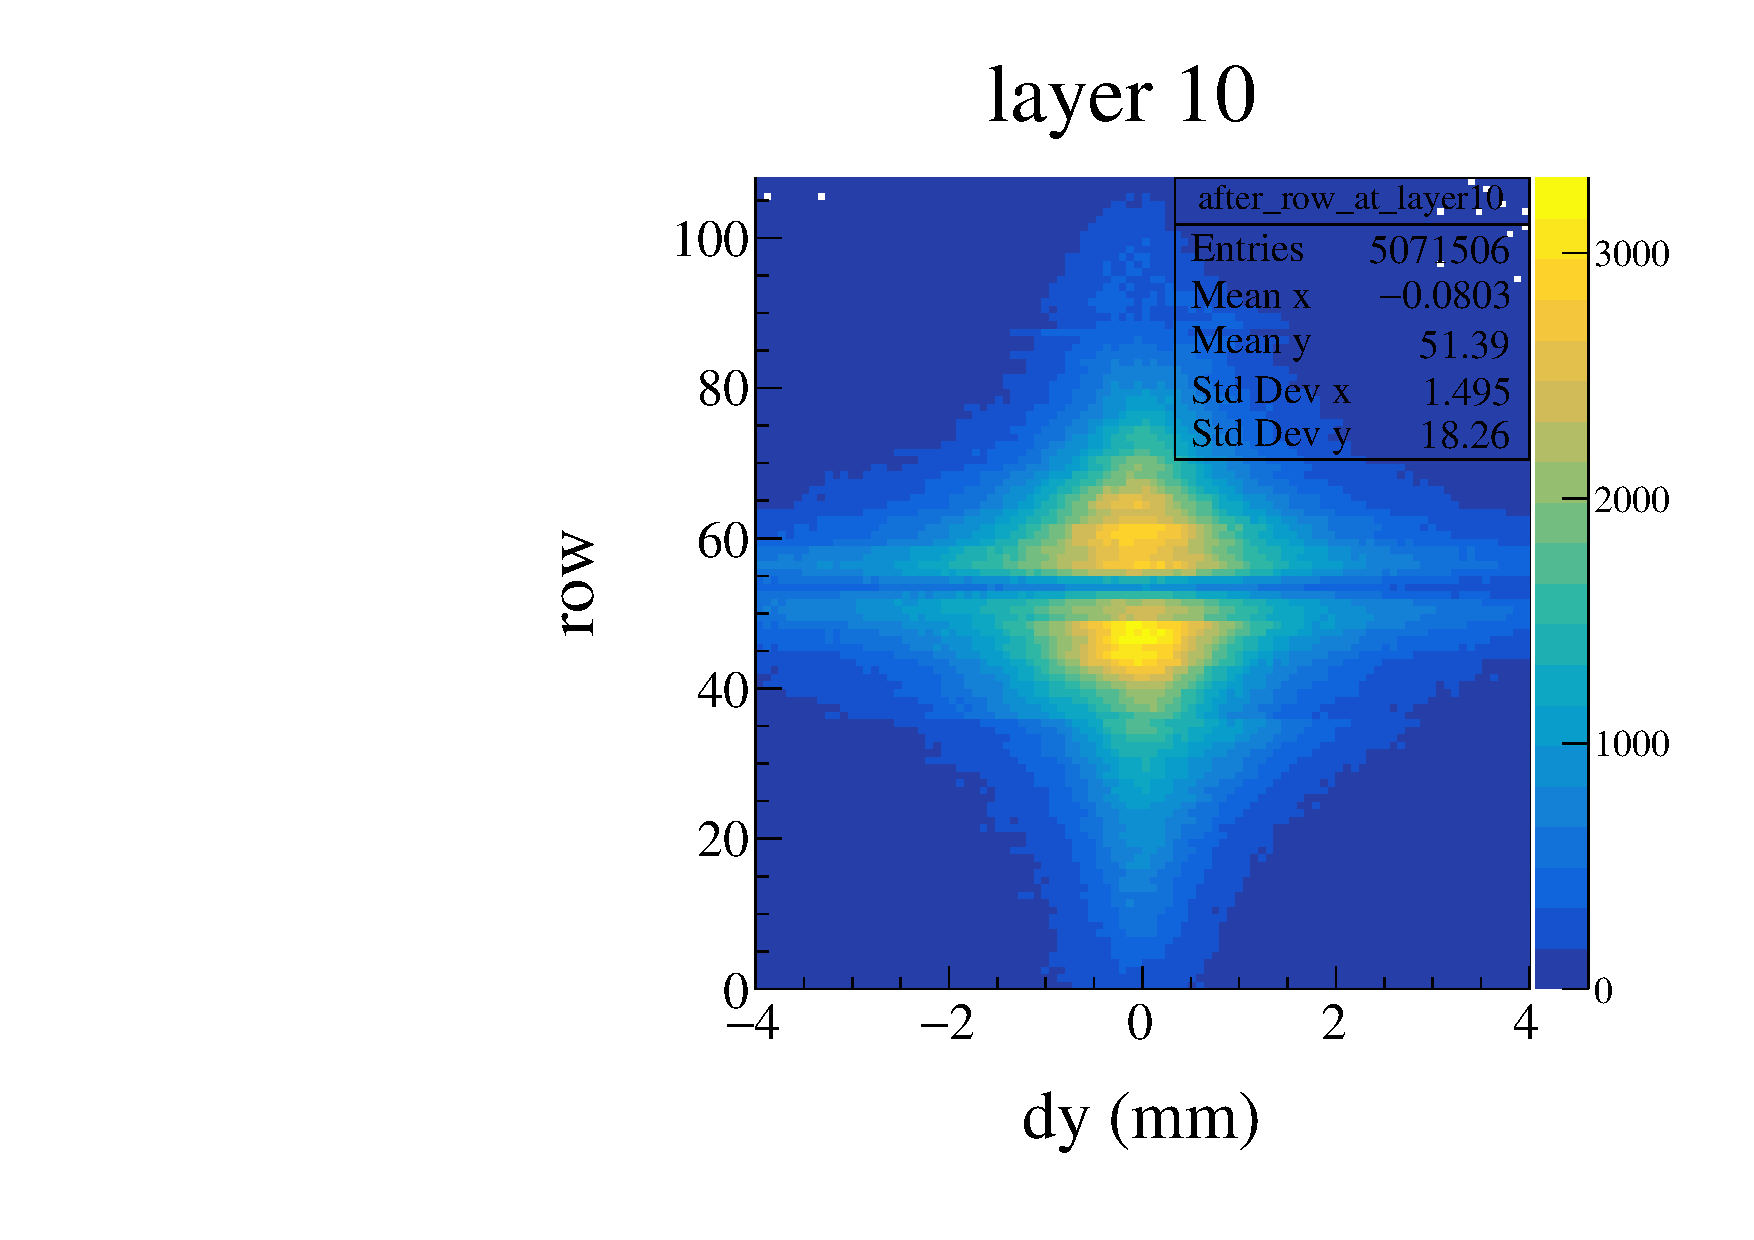
\includegraphics[width=0.33\textwidth]{after_row_at_layer10_yoffset.pdf}
    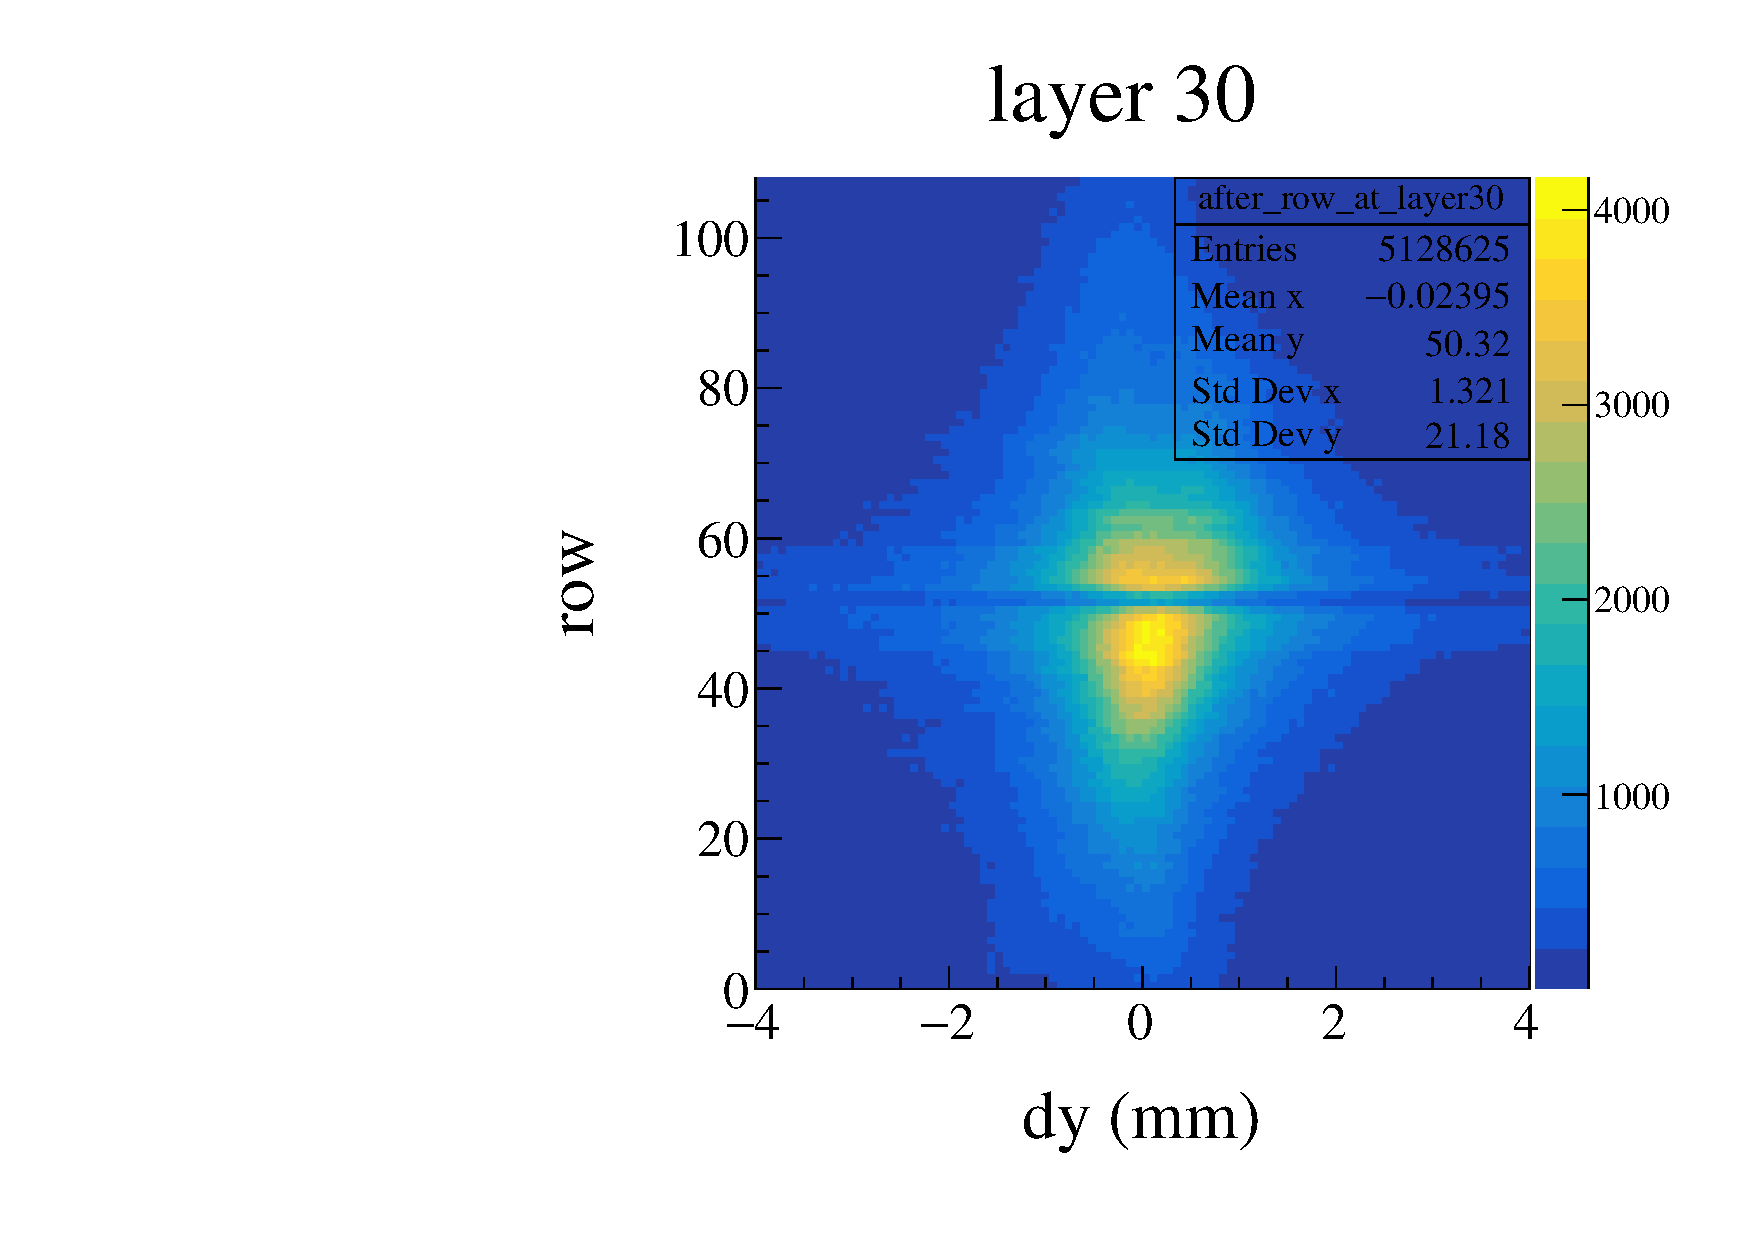
\includegraphics[width=0.33\textwidth]{after_row_at_layer30_yoffset.pdf}
    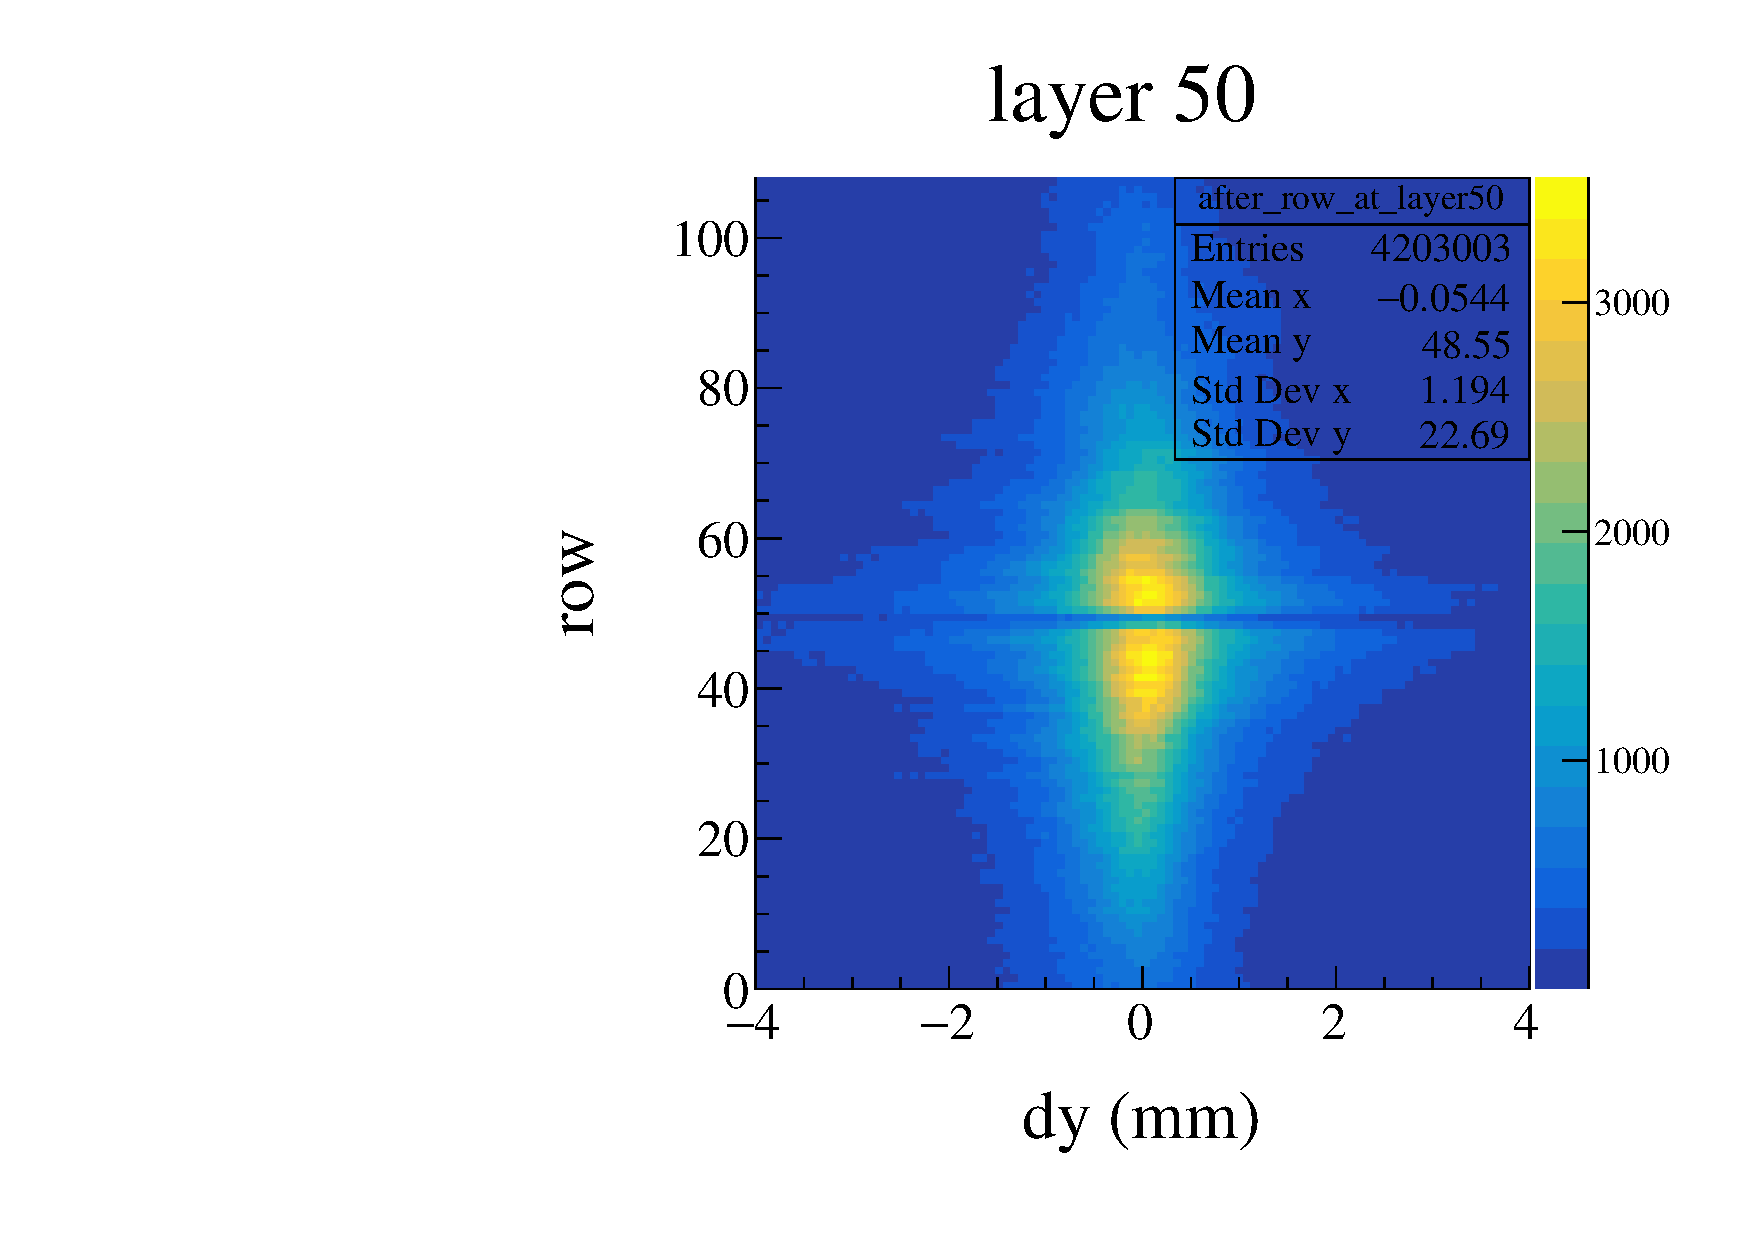
\includegraphics[width=0.33\textwidth]{after_row_at_layer50_yoffset.pdf}
 
    \caption{TBW\label{TBD}}
  \end{center}
  \label{fig:coboCorr}
\end{figure}



\begin{figure}[!htb]
    \centering
    \begin{subfigure}[t]{0.49\textwidth}
        \centering
        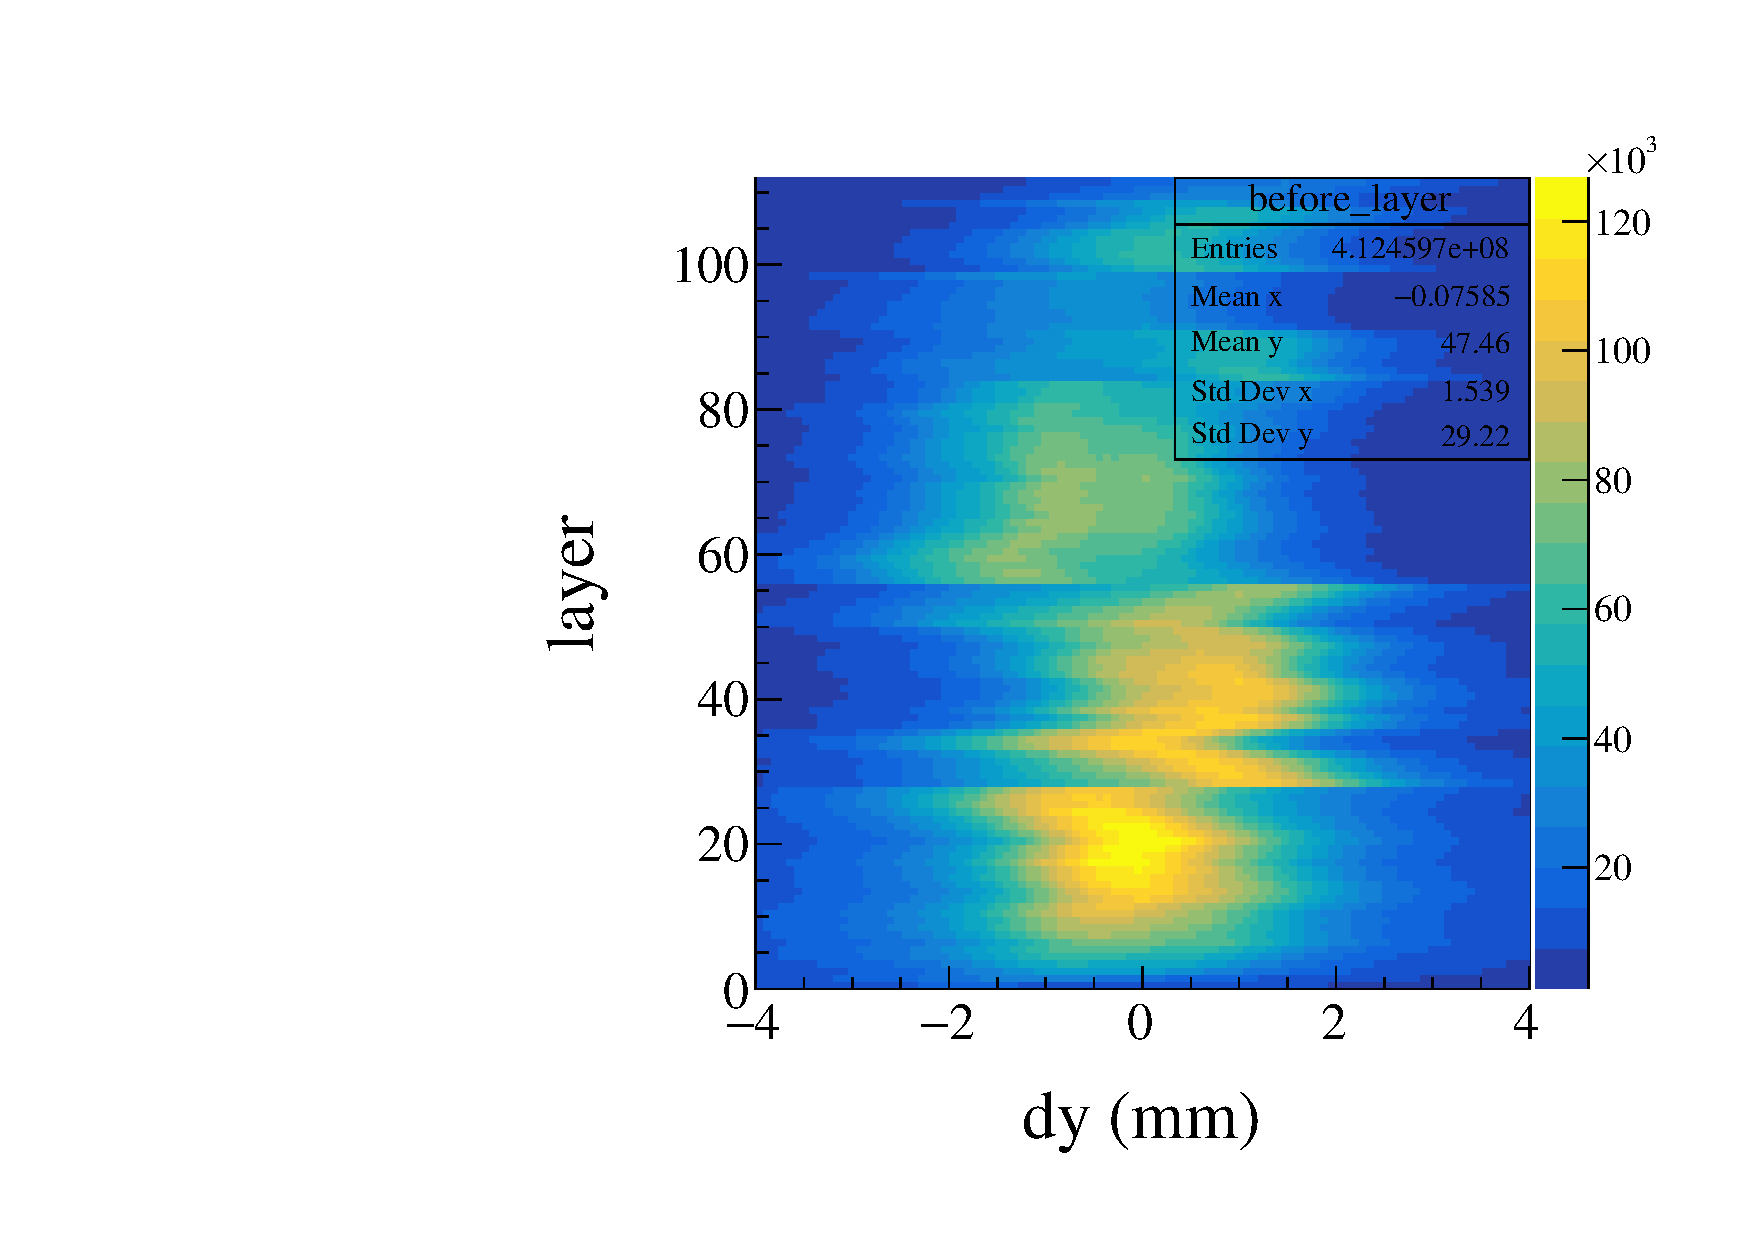
\includegraphics[width=\linewidth]{before_layer_yoffset.pdf}
        \caption{Y-offset for all layers before correction.} \label{fig:yoff_beforeLayer}
    \end{subfigure}
    \hfill
    \begin{subfigure}[t]{.49\textwidth}
        \centering
        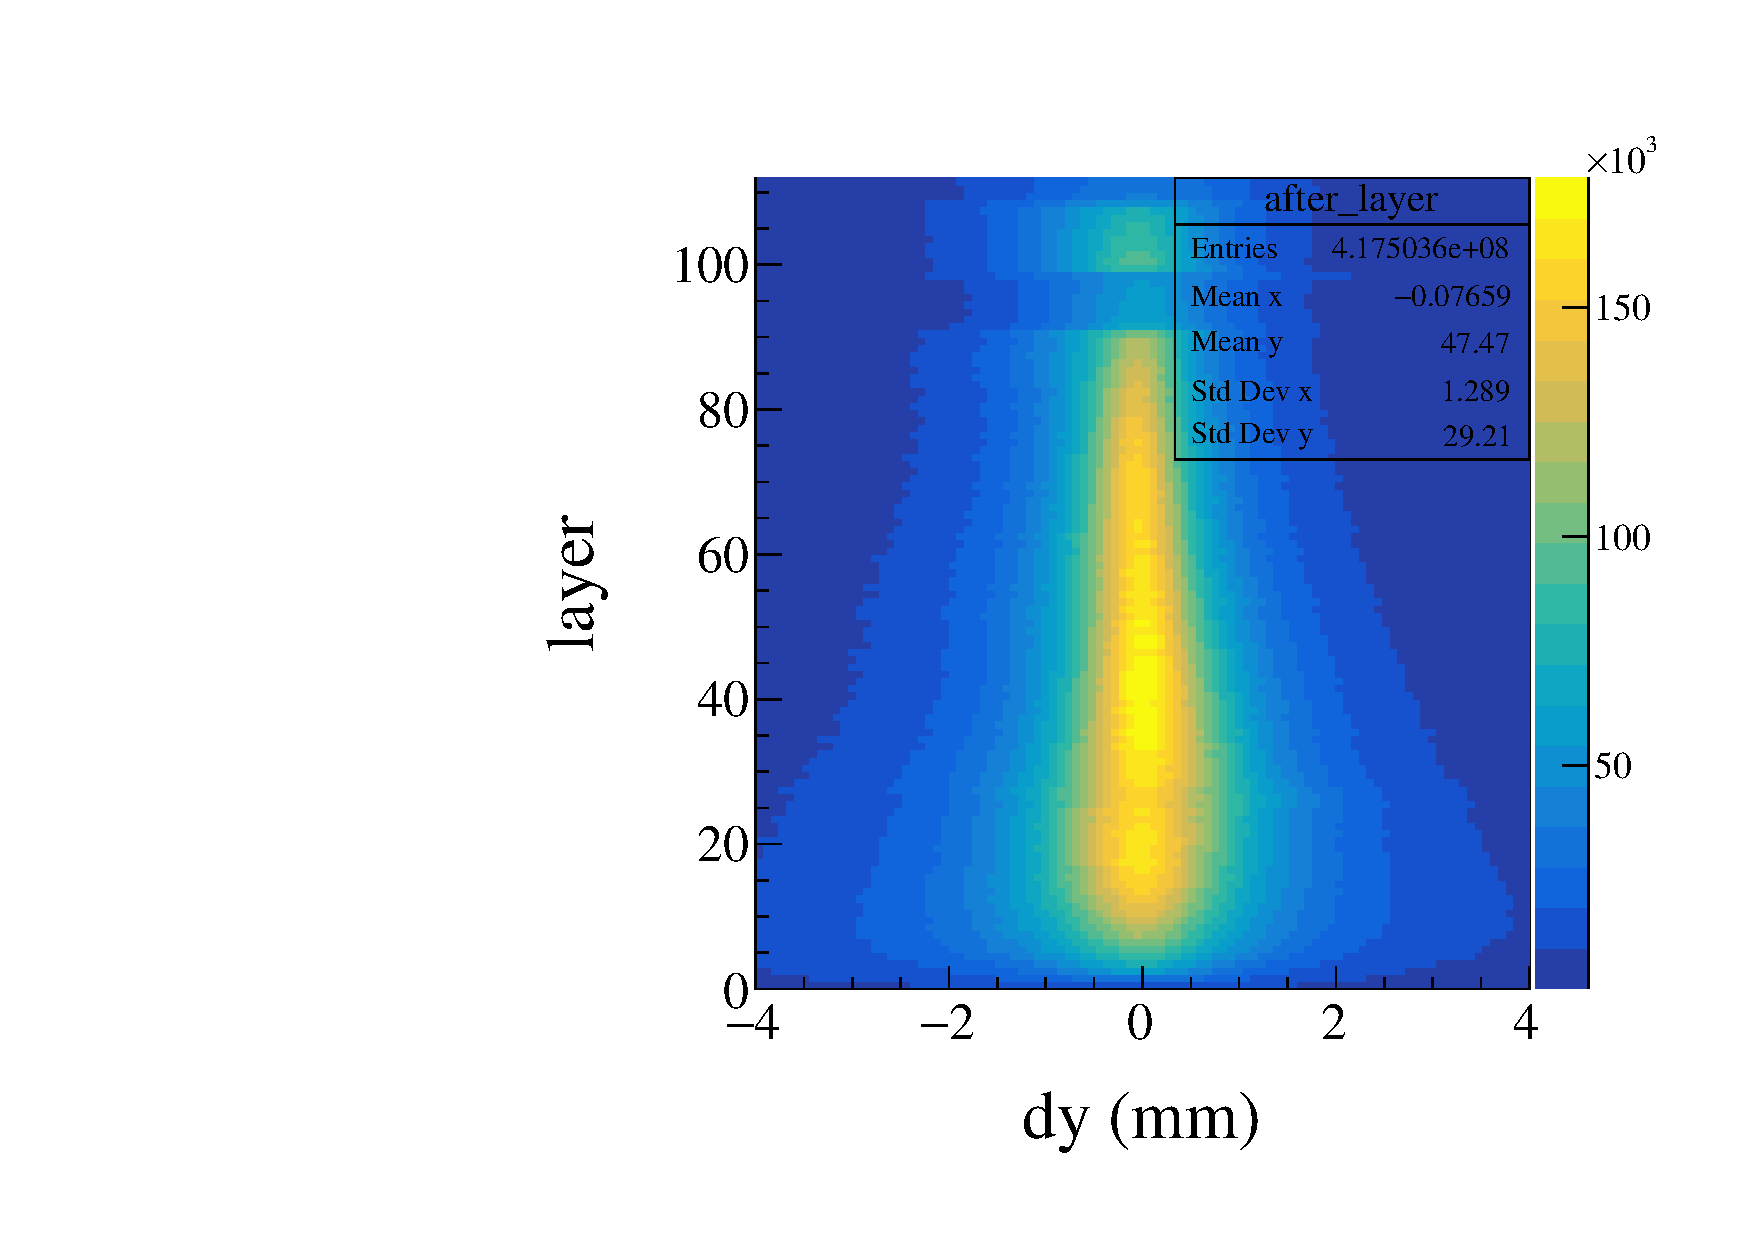
\includegraphics[width=\linewidth]{after_layer_yoffset.pdf} 
        \caption{Y-offset for all layers after correction.} \label{fig:yoff_afterLayer}
    \end{subfigure}
     \hfill
    \begin{subfigure}[t]{.49\textwidth}
        \centering
        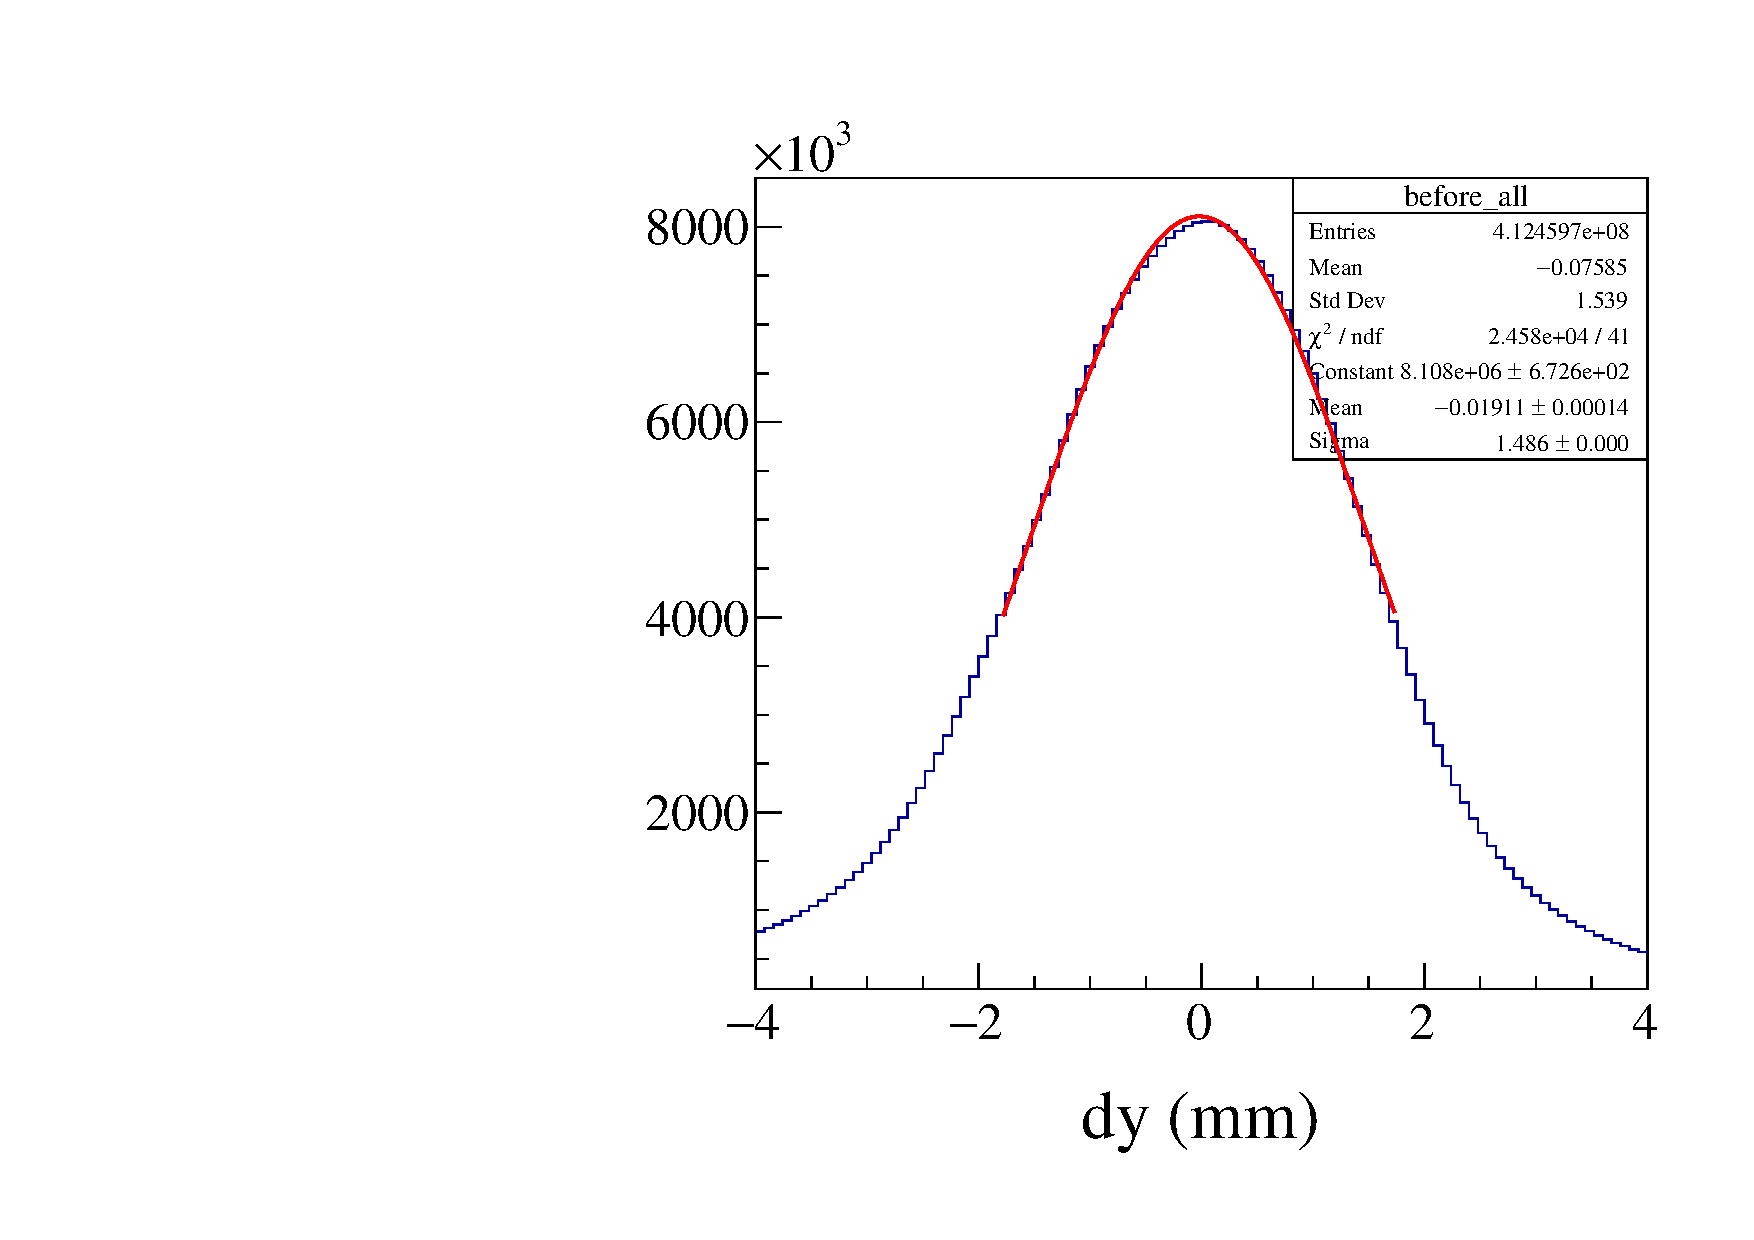
\includegraphics[width=\linewidth]{before_all_yoffset.pdf} 
        \caption{Distribution for all pads before correction.} \label{fig:yoff_allBefore}
    \end{subfigure}
    \hfill
    \begin{subfigure}[t]{.49\textwidth}
        \centering
        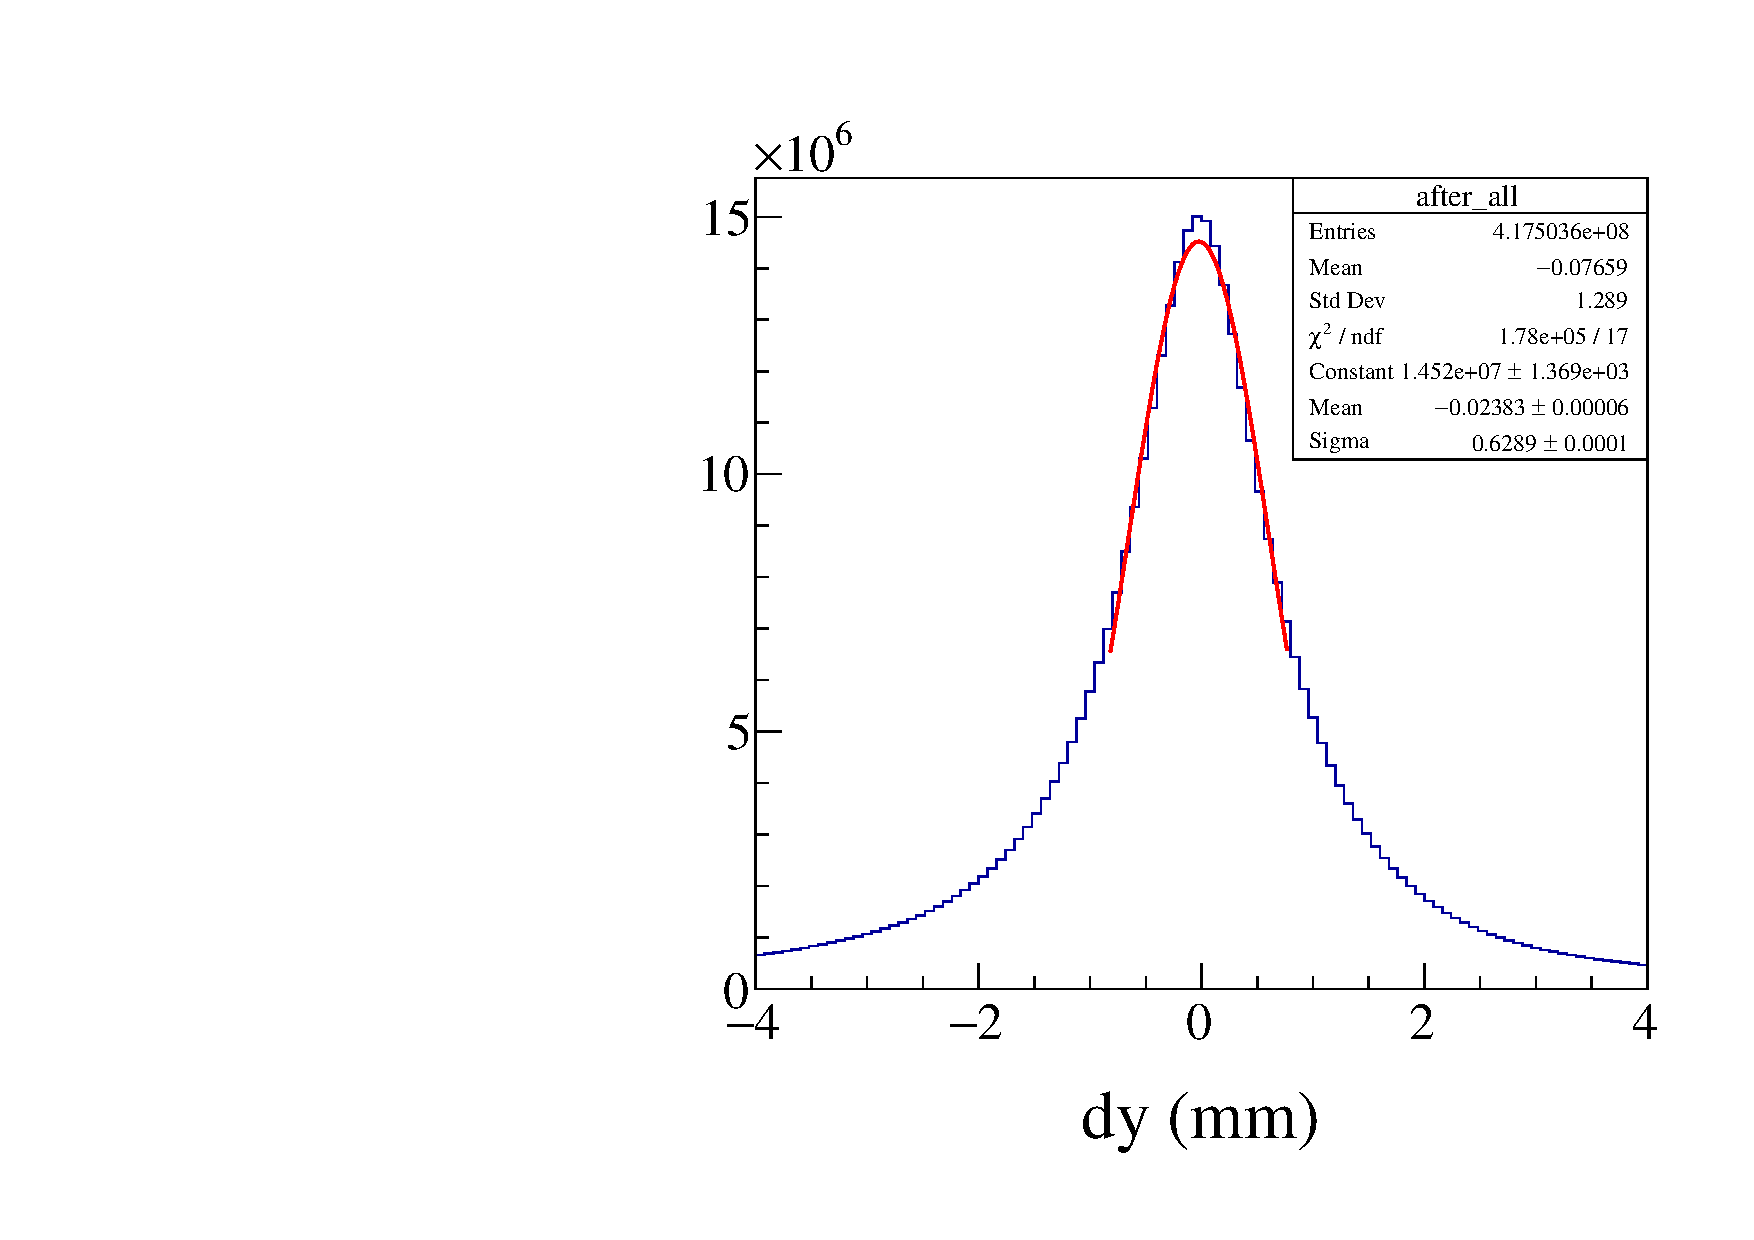
\includegraphics[width=\linewidth]{after_all_yoffset.pdf} 
        \caption{Distribution for all pads after correction.} \label{fig:yoff_allAfter}
    \end{subfigure}
    \caption{ }
\label{fig:yoff}
\end{figure}



\section{Efficiency Corrections}
\label{sec:efficiency}
Add Figures of efficiency vs angles in TPC polar angle plot for pions


Since the \spirit TPC is a fixed target experiment it's angular coverage is certainly not 4$\pi$. Because the target is several cm away from the widow of the field cage the geometric acceptance is not even 2$\pi$. The rectangular design complicates the calculation of the geometric acceptance, or the efficiency. Because of this there are regions of the TPC where it is impossible to reconstruct a track due to the geometric in these regions the efficiency is exactly 0. In the regions of non-zero efficiency, the efficiency is a function of at least three main parameters that define the phase space of a track, momentum $p$ and the two spherical lab angles $\theta_{Lab}$ and $\phi_{Lab}$. 

The track efficiency $\epsilon$ is calculated bin-by-bin and is simply written as, 
\begin{equation}
\epsilon = \frac{n_{reco}}{N},
\end{equation}

where $n_{reco}$ is the number of embedded tracks which are successfully reconstructed, and $N$ is the total number of input embedded tracks for that given bin. A track is defined to be successfully reconstructed if it exists in the correlation task described in \ref{sec:embedding}, and therefore meets the minimum criteria for an embedded track, and if it passes the various quality cuts performed on the experimental data set; this could be angular cuts, PID cuts, etc. The TPC response will introduce a finite resolution in both the angles and the momentum. Because of the final measured track could have migrated out of the input bin into another bin. The bin-by-bin correction method is only valid if this effect is small as compared with the size of the bin. If not a more complicated un-folding procedure is needed. The efficiency is defined as the number of all tracks that were reconstructed and passed the cuts successfully, even if some had migrated to other bins, the efficiency value is assumed to represent the center of the input MC bin.  
%TALK ABOUT BIN SIZES HEREE????? 

 Single MC tracks are embedded into a set of \num{e4} on target events and the measured output tracks are correlated to the input track from the embedding software. If the track split in the analysis software, and there are several tracks identified by the software as an embedded track, or part of one, we certainly cannot double count the track as the efficiency is  defined strictly as $\epsilon < 0$. In this case, the track with the minimum distance to vertex is taken for the purposes of calculating efficiency. This is because in the case the track splits, it is very rare for the later segments of the track to have a distance-to-vertex which originates from the target region. It's reasonable to assume the track with the minimum distance to vertex is the track that best represents the ``real" track. The embedded MC tracks are generated as a uniform distribution in $\theta$,$\phi$, and $p$, to ensure each bin has as similar number of input tracks $N$, giving approximately the same statistical error. Here the efficiency distribution is independent of the initial input distribution since we were careful to not assign tracks that migrated out of the input bin, into another bin, which would make the efficiency biased by the input distribution. 
 
\begin{figure}[!htb]
    \centering
    \begin{subfigure}[t]{0.49\textwidth}
        \centering
        \includegraphics[width=\linewidth]{pim_200_pol.png}
        \caption{Polar efficiency plot where $\theta$ is represented by the radius of the circle and $\phi$ is measured as the polar angle made between the y and x axis; this view is  best understood as looking at the TPC from the downstream point of view.} \label{fig:pim_pol_eff_ex}
    \end{subfigure}
    \hfill
    \begin{subfigure}[t]{.49\textwidth}
        \centering
        \includegraphics[width=\linewidth]{pim_200_efficiency.png} 
        \caption{Flattened angle plot} \label{fig:pim_flat_eff_ex}
    \end{subfigure}
  
\caption{Efficiency calculations for $\pi^-$ particle traveling at \SI{200}{\mega\eVperc}.}
\label{fig:pim_eff_ex}
\end{figure}
 
 
 
Figure~\ref{fig:pim_eff_ex} shows the efficiency calculated for $\pi^-$ tracks traveling with momentum \SI{200}{\mega\eVperc} as a function of the two laboratory angles. It is easiest to visualize the efficiency distribution first in a polar representation which is most like viewing the actual TPC progressing to a visualization that is easier to see the values. Figure~\ref{fig:pim_pol_eff_ex} shows the efficiency values plotted in a polar representation where $\theta_{Lab}$ is represented as the radial dimension and $\phi$ is represented as the polar angle. This way is best understood as if one looked at the TPC from the downstream point of view. Of course the vertical direction of the TPC,$\phi$=\ang{90}, is limited in vertical space, therefore tracks are not reconstructed well. The same is the case in downward going tracks, the region centered around $\phi$=\ang{270}. The best regions are seen by the high efficiency values which are left and right in the TPC where the rectangular TPC has the highest acceptance. Though this view is the most intuitive to think about in a physical geometry sense, the values of the efficiency in each bin are difficult to see. Figure~\ref{fig:pim_flat_eff_ex} shows the same efficiency plot but plotted in a more standard two dimensional plot. Here we can see even better the acceptance of downward going tracks , $\phi$=\ang{270}, is greater than the dip in upward going tracks, $\phi$=\ang{90}, due to the field cage being centered in the magnet and not in the TPC. 

The area enclosed by the red lines represent the region of the highest efficiency over the full region in $\theta_{Lab}$.  Since we take cuts similar to these in the real data, we assume the efficiency is independent of $\phi$ over these small regions. The efficiency then can be represented as just a function of the two remaining variables. Figure~\ref{fig:132_eff} shows the efficiency of $\pi^-$ and $\pi^+$ particles in the $\tin{132}{124}$ system and Fig.~\ref{fig:108_eff} for the $\tin{108}{112}$ system as a function of $\theta_{Lab}$ and momentum $p_{Lab}$. 



\begin{figure}[!htb]
    \centering
    \begin{subfigure}[t]{0.49\textwidth}
        \centering
        \includegraphics[width=\linewidth]{pim_132_efficiency.png}
        \caption{$\pi^-$ efficiency for $\tin{132}{124}$} \label{fig:pim_132_eff}
    \end{subfigure}
    \hfill
    \begin{subfigure}[t]{.49\textwidth}
        \centering
        \includegraphics[width=\linewidth]{pip_132_efficiency.png} 
        \caption{$\pi^+$ efficiency for $\tin{132}{124}$} \label{fig:pip_132_eff}
    \end{subfigure}
  
    \caption{ }
\label{fig:132_eff}
\end{figure}



\begin{figure}[!htb]
    \centering
    \begin{subfigure}[t]{0.49\textwidth}
        \centering
        \includegraphics[width=\linewidth]{pim_132_efficiency.png}
        \caption{$\pi^-$ efficiency for $\tin{108}{112}$} \label{fig:pim_108_eff}
    \end{subfigure}
    \hfill
    \begin{subfigure}[t]{.49\textwidth}
        \centering
        \includegraphics[width=\linewidth]{pip_108_efficiency.png} 
        \caption{$\pi^+$ efficiency for $\tin{108}{112}$} \label{fig:pip_108_eff}
    \end{subfigure}
  
    \caption{ }
\label{fig:108_eff}
\end{figure}

The efficiency correction is applied track-by-track, where the efficiency of the i-th track $\epsilon_i$ is retrieved from the database. The correction factor $C_i$ is defined as,

\begin{equation}
C_i = \epsilon_i^{-1}.
\end{equation}

The track is then weighted by the factor $C_i$ when plotting in any type of graph for any observable. 